%  LaTeX support: latex@mdpi.com 
%  For support, please attach all files needed for compiling as well as the log file, and specify your operating system, LaTeX version, and LaTeX editor.

%=================================================================
\documentclass[make,article,accept,pdftex,moreauthors]{Definitions/mdpi} 
%\documentclass[preprints,article,submit,pdftex,moreauthors]{Definitions/mdpi} 
% For posting an early version of this manuscript as a preprint, you may use "preprints" as the journal. Changing "submit" to "accept" before posting will remove line numbers.

%--------------------
% Class Options:
%--------------------
%----------
% journal
%----------
% Choose between the following MDPI journals:
% accountaudit, acoustics, actuators, addictions, adhesives, admsci, adolescents, aerobiology, aerospace, agriculture, agriengineering, agrochemicals, agronomy, ai, air, algorithms, allergies, alloys, amh, analytica, analytics, anatomia, anesthres, animals, antibiotics, antibodies, antioxidants, applbiosci, appliedchem, appliedmath, appliedphys, applmech, applmicrobiol, applnano, applsci, aquacj, architecture, arm, arthropoda, arts, asc, asi, astronomy, atmosphere, atoms, audiolres, automation, axioms, bacteria, batteries, bdcc, behavsci, beverages, biochem, bioengineering, biologics, biology, biomass, biomechanics, biomed, biomedicines, biomedinformatics, biomimetics, biomolecules, biophysica, biosensors, biosphere, biotech, birds, blockchains, bloods, blsf, brainsci, breath, buildings, businesses, cancers, carbon, cardiogenetics, catalysts, cells, ceramics, challenges, chemengineering, chemistry, chemosensors, chemproc, children, chips, cimb, civileng, cleantechnol, climate, clinbioenerg, clinpract, clockssleep, cmd, cmtr, coasts, coatings, colloids, colorants, commodities, complications, compounds, computation, computers, condensedmatter, conservation, constrmater, cosmetics, covid, crops, cryo, cryptography, crystals, csmf, ctn, curroncol, cyber, dairy, data, ddc, dentistry, dermato, dermatopathology, designs, devices, diabetology, diagnostics, dietetics, digital, disabilities, diseases, diversity, dna, drones, dynamics, earth, ebj, ecm, ecologies, econometrics, economies, education, eesp, ejihpe, electricity, electrochem, electronicmat, electronics, encyclopedia, endocrines, energies, eng, engproc, ent, entomology, entropy, environments, epidemiologia, epigenomes, esa, est, famsci, fermentation, fibers, fintech, fire, fishes, fluids, foods, forecasting, forensicsci, forests, fossstud, foundations, fractalfract, fuels, future, futureinternet, futureparasites, futurepharmacol, futurephys, futuretransp, galaxies, games, gases, gastroent, gastrointestdisord, gastronomy, gels, genealogy, genes, geographies, geohazards, geomatics, geometry, geosciences, geotechnics, geriatrics, glacies, grasses, greenhealth, gucdd, hardware, hazardousmatters, healthcare, hearts, hemato, hematolrep, heritage, higheredu, highthroughput, histories, horticulturae, hospitals, humanities, humans, hydrobiology, hydrogen, hydrology, hygiene, idr, iic, ijerph, ijfs, ijgi, ijmd, ijms, ijns, ijpb, ijt, ijtm, ijtpp, ime, immuno, informatics, information, infrastructures, inorganics, insects, instruments, inventions, iot, j, jal, jcdd, jcm, jcp, jcs, jcto, jdad, jdb, jeta, jfb, jfmk, jimaging, jintelligence, jlpea, jmahp, jmmp, jmms, jmp, jmse, jne, jnt, jof, joitmc, joma, jop, jor, journalmedia, jox, jpbi, jpm, jrfm, jsan, jtaer, jvd, jzbg, kidney, kidneydial, kinasesphosphatases, knowledge, labmed, laboratories, land, languages, laws, life, lights, limnolrev, lipidology, liquids, literature, livers, logics, logistics, lubricants, lymphatics, machines, macromol, magnetism, magnetochemistry, make, marinedrugs, materials, materproc, mathematics, mca, measurements, medicina, medicines, medsci, membranes, merits, metabolites, metals, meteorology, methane, metrics, metrology, micro, microarrays, microbiolres, microelectronics, micromachines, microorganisms, microplastics, microwave, minerals, mining, mmphys, modelling, molbank, molecules, mps, msf, mti, multimedia, muscles, nanoenergyadv, nanomanufacturing, nanomaterials, ncrna, ndt, network, neuroglia, neurolint, neurosci, nitrogen, notspecified, nursrep, nutraceuticals, nutrients, obesities, oceans, ohbm, onco, oncopathology, optics, oral, organics, organoids, osteology, oxygen, parasites, parasitologia, particles, pathogens, pathophysiology, pediatrrep, pets, pharmaceuticals, pharmaceutics, pharmacoepidemiology, pharmacy, philosophies, photochem, photonics, phycology, physchem, physics, physiologia, plants, plasma, platforms, pollutants, polymers, polysaccharides, populations, poultry, powders, preprints, proceedings, processes, prosthesis, proteomes, psf, psych, psychiatryint, psychoactives, psycholint, publications, purification, quantumrep, quaternary, qubs, radiation, reactions, realestate, receptors, recycling, regeneration, religions, remotesensing, reports, reprodmed, resources, rheumato, risks, robotics, rsee, ruminants, safety, sci, scipharm, sclerosis, seeds, sensors, separations, sexes, signals, sinusitis, siuj, skins, smartcities, sna, societies, socsci, software, soilsystems, solar, solids, spectroscj, sports, standards, stats, std, stresses, surfaces, surgeries, suschem, sustainability, symmetry, synbio, systems, tae, targets, taxonomy, technologies, telecom, test, textiles, thalassrep, therapeutics, thermo, timespace, tomography, tourismhosp, toxics, toxins, transplantology, transportation, traumacare, traumas, tropicalmed, universe, urbansci, uro, vaccines, vehicles, venereology, vetsci, vibration, virtualworlds, viruses, vision, waste, water, wem, wevj, wild, wind, women, world, youth, zoonoticdis

%---------
% article
%---------
% The default type of manuscript is "article", but can be replaced by: 
% abstract, addendum, article, benchmark, book, bookreview, briefcommunication, briefreport, casereport, changes, clinicopathologicalchallenge, comment, commentary, communication, conceptpaper, conferenceproceedings, correction, conferencereport, creative, datadescriptor, discussion, entry, expressionofconcern, extendedabstract, editorial, essay, erratum, fieldguide, hypothesis, interestingimages, letter, meetingreport, monograph, newbookreceived, obituary, opinion, proceedingpaper, projectreport, reply, retraction, review, perspective, protocol, shortnote, studyprotocol, supfile, systematicreview, technicalnote, viewpoint, guidelines, registeredreport, tutorial,  giantsinurology, urologyaroundtheworld
% supfile = supplementary materials

%----------
% submit
%----------
% The class option "submit" will be changed to "accept" by the Editorial Office when the paper is accepted. This will only make changes to the front page (e.g., the logo of the journal will get visible), the headings, and the copyright information. Also, line numbering will be removed. Journal info and pagination for accepted papers will also be assigned by the Editorial Office.

%------------------
% moreauthors
%------------------
% If there is only one author, the class option oneauthor should be used. Otherwise, use the class option moreauthors.

%---------
% pdftex
%---------
% The option pdftex is for use with pdfLaTeX. Remove "pdftex" for (1) compiling with LaTeX & dvi2pdf (if eps figures are used) or for (2) compiling with XeLaTeX.

%=================================================================
% MDPI internal commands - do not modify
\firstpage{1} 
\makeatletter 
\setcounter{page}{\@firstpage} 
\makeatother
\pubvolume{1}
\issuenum{1}
\articlenumber{0}
\pubyear{2025}
\copyrightyear{2025}
\externaleditor{Firstname Lastname} % More than 1 editor, please add `` and '' before the last editor name
\datereceived{9 October 2025} 
\daterevised{1 November 2025} % Comment out if no revised date
\dateaccepted{7 November 2025} 
\datepublished{ } 
%\datecorrected{} % For corrected papers: "Corrected: XXX" date in the original paper.
%\dateretracted{} % For retracted papers: "Retracted: XXX" date in the original paper.
\hreflink{https://doi.org/} % If needed use \linebreak
%\doinum{}
%\pdfoutput=1 % Uncommented for upload to arXiv.org
%\CorrStatement{yes}  % For updates
%\longauthorlist{yes} % For many authors that exceed the left citation part
%\IsAssociation{yes} % For association journals

%=================================================================
% Add packages and commands here. The following packages are loaded in our class file: fontenc, inputenc, calc, indentfirst, fancyhdr, graphicx, epstopdf, lastpage, ifthen, float, amsmath, amssymb, lineno, setspace, enumitem, mathpazo, booktabs, titlesec, etoolbox, tabto, xcolor, colortbl, soul, multirow, microtype, tikz, totcount, changepage, attrib, upgreek, array, tabularx, pbox, ragged2e, tocloft, marginnote, marginfix, enotez, amsthm, natbib, hyperref, cleveref, scrextend, url, geometry, newfloat, caption, draftwatermark, seqsplit
% cleveref: load \crefname definitions after \begin{document}

%\usepackage{cite}
\usepackage{xurl} % best for url-breaking, especially long URLs
%\usepackage[hidelinks]{hyperref}
\usepackage{amsfonts}
%\usepackage{algorithmic}
\usepackage{graphicx}
\usepackage{textcomp}
\usepackage{makecell}

\usepackage{algorithm}
\usepackage{algpseudocode}

\usepackage{amsmath}
\usepackage{amssymb}
\usepackage[T1]{fontenc}

\usepackage[utf8]{inputenc}

\usepackage{amsmath,amssymb}

\usepackage[russian,english]{babel}
\usepackage{upgreek}
\DeclareMathSymbol{\mhyphen}{\mathord}{AMSa}{"39}

%=================================================================
% Please use the following mathematics environments: Theorem, Lemma, Corollary, Proposition, Characterization, Property, Problem, Example, ExamplesandDefinitions, Hypothesis, Remark, Definition, Notation, Assumption
%% For proofs, please use the proof environment (the amsthm package is loaded by the MDPI class).

%=================================================================
% Full title of the paper (Capitalised)
\Title{Extreme Multi-Label Text Classification for Less-Represented Languages and Low-Resource Environments: Advances and Lessons Learned}

% MDPI internal command: Title for citation in the left column
\TitleCitation{Extreme Multi-Label Text Classification for Less-Represented Languages}

% Author Orchid ID: enter ID or remove command
\newcommand{\orcidauthorA}{0009-0008-8016-9530} % Add \orcidA{} behind the author's name
\newcommand{\orcidauthorB}{0000-0002-9916-8756} % Add \orcidB{} behind the author's name
\newcommand{\orcidauthorC}{0000-0002-7330-0579} % Add \orcidC{} behind the author's name
\newcommand{\orcidauthorD}{0000-0002-4380-0863} % Add \orcidD{} behind the author's name
\newcommand{\orcidauthorE}{0000-0002-9995-7093} % Add \orcidE{} behind the author's name
\newcommand{\orcidauthorF}{0000-0003-2297-1273} % Add \orcidF{} behind the author's name

% Authors, for the paper (add full first names)
\Author{Nikola Ivačič
 $^{1,2,}$*\orcidA{}, Blaž Škrlj $^{1}$\orcidB{}, Boshko Koloski $^{1,2}$\orcidC{}, Senja Pollak $^{1,2}$\orcidD{}, Nada Lavrač $^{1,3}$\orcidE{}\linebreak and Matthew Purver $^{1,4}$\orcidF{}}

%\longauthorlist{yes}

% MDPI internal command: Authors, for metadata in PDF
\AuthorNames{Nikola Ivačič, Blaž Škrlj, Boshko Koloski, Senja Pollak, Nada Lavrač and Matthew Purver}

% MDPI internal command: Authors, for citation in the left column, only choose one of them below according to the journal style

% If this is an ACS-style journal (Except for the above Chicago and APA journals, all others are in the ACS format): 
% Lastname, F.; Lastname, F.; Lastname, F.
\AuthorCitation{Ivačič, N.; Škrlj, B.; Koloski,~B.; Pollak, S.; Lavrač, N.; Purver, M.}

% Affiliations/Addresses (Add [1] after \address if there is only one affiliation.)
\address{%
$^{1}$ \quad Department of Knowledge Technologies, Jožef Stefan Institute, Jamova cesta 39, 1000 Ljubljana, Slovenia; blaz.skrlj@ijs.si
 (B.Š.); boshko.koloski@ijs.si (B.K.); senja.pollak@ijs.si (S.P.); nada.lavrac@ijs.si (N.L.); m.purver@qmul.ac.uk (M.P.)\\
$^{2}$ \quad Jožef Stefan International Postgraduate School, Jamova cesta 39, 1000 Ljubljana, Slovenia\\
$^{3}$ \quad Faculty of Computer and Information Science, University of Ljubljana, Večna pot 113, 1000 Ljubljana, Slovenia\\
$^{4}$ \quad School of Electronic Engineering and Computer Science, Queen Mary University of London,\linebreak London E1 4NS, UK
}

% Contact information of the corresponding author
\corres{Correspondence: nikola.ivacic@ijs.si}

% Current address and/or shared authorship
%\firstnote{Current address: Affiliation.}  
% Current address should not be the same as any items in the Affiliation section.

%\secondnote{These authors contributed equally to this work.}
% The commands \thirdnote{} till \eighthnote{} are available for further notes.

%\simplesumm{} % Simple summary

%\conference{} % An extended version of a conference paper

% Abstract (Do not insert blank lines, i.e.,~\\) 
%\abstract{
%The rapid advancement of Large Language Models (LLMs) has significantly impacted the field of Natural Language Processing (NLP). 
%While recent trends focus on developing extremely large, multimodal models with vast numbers of parameters, there is also increasing interest in more efficient Small Language Models (SLMs) that can operate outside large data centre clusters. 
%However, recent SLMs with up to three billion parameters, such as LLaMA or Phi, are predominantly trained in high-resource languages, such as English, which limits their applicability for industries that require robust NLP solutions for less-represented languages and low-resource settings, particularly those requiring low latency and adaptability to evolving label spaces.
%This paper explores a retrieval-based approach to multi-label text classification (MLC) for a media monitoring dataset, focusing on less-represented languages such as Slovene. 
%This dataset presents an extreme MLC challenge, with instances labelled using up to twelve thousand categories. 
%The proposed method, which combines retrieval with computationally efficient prediction, effectively addresses challenges related to multilinguality, resource constraints, and frequent label changes. 
%We adopt a model-agnostic approach that does not rely on a specific model architecture or language selection. 
%Our results demonstrate that techniques from the extreme multi-label text classification (XMC) domain outperform traditional Transformer-based encoder models, particularly in handling dynamic label spaces without requiring continuous fine-tuning. 
%Additionally, we highlight the effectiveness of this approach in scenarios involving rare labels, where baseline models struggle with generalisation. The paper also contributes a reflection on the lessons learned from experiments in extreme multi-label text classification for less-represented languages and low-resource environments.}
\abstract{
Amid ongoing efforts to develop extremely large, multimodal models, there is increasing interest in efficient Small Language Models (SLMs) that can operate without reliance on large data-centre infrastructure. However, recent SLMs (e.g., LLaMA or Phi) with up to three billion parameters are predominantly trained in high-resource languages, such as English, which limits their applicability to industries that require robust NLP solutions for less-represented languages and low-resource settings, particularly those requiring low latency and adaptability to evolving label spaces. 
This paper examines a retrieval-based approach to multi-label text classification (MLC) for a media monitoring dataset, with a particular focus on less-represented languages, such as Slovene. 
This dataset presents an extreme MLC challenge, with instances labelled using up to twelve thousand categories. 
The proposed method, which combines retrieval with computationally efficient prediction, effectively addresses challenges related to multilinguality, resource constraints, and frequent label changes. 
We adopt a model-agnostic approach that does not rely on a specific model architecture or language selection. Our results demonstrate that techniques from the extreme multi-label text classification (XMC) domain outperform traditional Transformer-based encoder models, particularly in handling dynamic label spaces without requiring continuous fine-tuning. Additionally, we highlight the effectiveness of this approach in scenarios involving rare labels, where baseline models struggle with generalisation. 
%The paper also contributes a reflection on the lessons learned from experiments in extreme multi-label text classification for less-represented languages and low-resource environments.
}

% ACM Computing Classification System (CCS) 2012
%\ccsdesc[500]{Information systems~Retrieval models and ranking}
%\ccsdesc[500]{Computing methodologies~Natural language processing}
%\ccsdesc[300]{Information systems~Clustering and classification}
%\ccsdesc[300]{Information systems~Multilingual and cross-lingual retrieval}
%\ccsdesc[300]{Computing methodologies~Supervised learning by classification}
%\ccsdesc[100]{Information systems~Similarity measures}
%\ccsdesc[100]{Computing methodologies~Neural networks}
%\ccsdesc[100]{Information systems~Top-k retrieval in databases}

% Keywords
\keyword{multi-label text classification; multilingual text classification; retrieval;\linebreak low-resource environments; less-represented languages; media monitoring; news topics} 

%%%%%%%%%%%%%%%%%%%%%%%%%%%%%%%%%%%%%%%%%%
% Different journals have different requirements. Please check the specific journal guidelines in the "Instructions for Authors" on the journal's official website.
%\addhighlights{yes}
%\renewcommand{\addhighlights}{%
%
%\noindent The goal is to increase the discoverability and readability of the article via search engines and other scholars. Highlights should not be a copy of the abstract, but a concise text that allows the reader to quickly find out what the article is about and what can be cited from it. Each of these parts should be devoted to up to 2 bullet points.\vspace{3pt}\\
%\textbf{What are the main findings?}
% \begin{itemize}[labelsep=2.5mm,topsep=-3pt]
% \item First bullet.
% \item Second bullet.
% \end{itemize}\vspace{3pt}
%\textbf{What is the implication of the main finding?}
% \begin{itemize}[labelsep=2.5mm,topsep=-3pt]
% \item First bullet.
% \item Second bullet.
% \end{itemize}
%}

%%%%%%%%%%%%%%%%%%%%%%%%%%%%%%%%%%%%%%%%%%
\begin{document}

%%%%%%%%%%%%%%%%%%%%%%%%%%%%%%%%%%%%%%%%%%
\section{Introduction}
\label{sec:introduction}

In today's fast-paced world, media monitoring and analysis require near real-time capabilities to deliver timely and relevant information. 
This process involves categorising articles by content, attaching metadata tags, and~synthesising information from multiple news sources~\citep{rupnik2016news, zang2022event_detection,yoon2023story_detection}. 
Advanced Natural Language Processing (NLP) techniques are well-suited for these tasks, enabling the development of personalised news recommendation systems, automated content summarisation, and~effective organisation and prioritisation of news~items. 

However, the~operational reality of media monitoring—processing very large daily article volumes under strict latency and cost budgets—renders general-purpose LLMs ill-suited for sustained production use. High per-token inference costs, accelerator dependence, and~third-party API constraints (including privacy, availability, and~rate limits) conflict with industry requirements for low-latency, on-premises, and~cost-predictable pipelines. 
These constraints are amplified for less-represented languages, where LLM coverage and training data are limited, and~for extreme multi-label settings with frequent label changes, where continuous fine-tuning is infeasible. This motivates our focus on efficient, retrieval-based MLC that operates on consumer-grade hardware while maintaining robustness across multilingual and low-resource contexts.
%The media monitoring industry in certain regions faces increasing challenges due to evolving market dynamics and rising operational expenses. 
%These pressures limit the ability to invest in the extensive hardware infrastructure required to deploy advanced NLP technologies. In response, research efforts increasingly focus on designing solutions that prioritise computational efficiency, enabling deployment on consumer-grade hardware~\citep{lu2025smalllanguagemodelssurvey}. 
%Such approaches balance performance with practicality, supporting resource-conscious and sustainable implementation strategies while making machine intelligence more accessible to a broader audience.

Transformer-based models have become the dominant NLP approach, evolving from encoder architectures, such as BERT~\citep{devlin2018bert}, to~generative text-to-text models, such as T5~\citep{raffel2020exploring}, GPT~\citep{brown2020language}, and~LLaMA~\citep{touvron2023llama2openfoundation}, excelling in tasks such as text generation and classification~\citep{tarekegn2024deeplearningmultilabellearning,li2022surveytextclassification}. 
Current LLM trends follow two paths: large-scale foundation models with high computational costs~\citep{dubey2024llama3herdmodels,openai2024gpt4technicalreport, geminiteam2024geminifamilyhighlycapable} and smaller, efficient generative models (SLMs) designed for resource-limited settings~\citep{abdin2024phi4technicalreport, gemma_2025}.
Although SLMs are a promising option for constrained environments~\citep{subramanian2025smalllanguagemodelsslms}, their effectiveness in real-world, data-intensive, multi-label classification is limited~\citep{vajjala2025textclassificationllmera}, particularly when handling multiple languages and a large label space.
More specifically, the~available pre-trained SLMs still lack pre-training in target South Slavic languages and require techniques such as pruning, knowledge distillation~\citep{muralidharan2024compact, gu2024minillmknowledgedistillationlarge}, or~quantisation~\citep{malinovskii2024pvtuningstraightthroughestimationextreme} to run on consumer-grade hardware, often facing licensing and latency challenges in deployment.
Most often, generative LLMs for text classification or information retrieval (IR) are used in the context of synthetic data generation~\citep{kuzman2025LLMteacher, vajjala2025textclassificationllmera}.

This paper introduces an approach for developing a classification system tailored to news articles, capable of accommodating longer text lengths, supporting multiple languages, and~adapting to near-real-time label changes. 
To address these challenges, we constructed and down-sampled a large-scale dataset, NewsMon, obtained from a targeted Slovenian media monitoring industry archive. 
The original dataset, with~over one million data points and more than ten thousand labels categorising client concepts under the term ``client topics'', was adopted as the basis for developing our classification framework.
We formulated the problem as a multi-label classification task, where client-defined ``topics'' are treated as~labels. 

Given the inherent complexity of the dataset and its large, long-tailed label space, our methodology draws upon research in Extreme Multi-Label Classification (XMC).
We formulated our task within the XMC framework, as~the classification problem exhibits poor scalability with an increasing number of labels, making traditional one-versus-all methods largely infeasible in this setting~\citep{dasgupta2025reviewextrememultilabelclassification}.
In particular, we built upon the Retrieval-Augmented Encoders for XMC (RAE-XMC) framework~\citep{wang2025retrievalaugmentedencodersextrememultilabel} to develop our solution.
This framework employs a single-encoder architecture, where a single encoder is used to embed both the training examples and the label~descriptions. 

In this work, we address the following research questions on the task of client custom topic~classification:
\begin{enumerate}
    \item[RQ1] Can we overcome the traditional one-versus-all (OVA) Transformer Encoder (TE) classification baselines in a multilingual setting?
    \item[RQ2] How effective is the method without label description embeddings?
    \item[RQ3] Can pre-trained multilingual IR models be used effectively without fine-tuning?
    \item[RQ4] Can we improve the method by incorporating additional contrastive learning with hard negative mining?
\end{enumerate}

In summary, this study contributes the following advances and lessons~learned: 
\begin{itemize}
\item The study demonstrates that IR models can outperform end-to-end fine-tuned models on specific datasets when working with an extremely large number of labels, providing a computationally efficient approach to scaling to an arbitrary number of labels.
\item The experiments demonstrate that a significant gap remains between end-to-end fine-tuned models and IR models on less-represented non-English tasks, rendering IR models more suitable for these tasks in the XMC setting.
\item When evaluating the modified RAE-XMC method on a novel and distinct dataset in a multilingual setting, we demonstrate that employing contrastive learning with precomputed hard negatives is beneficial.
\item Additionally, we demonstrate the effectiveness of the approach without relying on label space embeddings while also handling longer texts than those typically considered in traditional XMC tasks. 
\item Finally, by~comparing the performance of the modified RAE-XMC in less-represented, non-English languages, we demonstrate that the method can be easily adapted to multilingual settings, without~significant loss in performance, as~shown in the case \mbox{of Slovene. }
\end{itemize}

The key novelty of this work is the application of an information-retrieval-based approach to multilingual, multi-label text classification, specifically targeting low-resource languages and large or evolving label spaces.
Unlike conventional end-to-end fine-tuned models, the~proposed IR-based method performs competitively even without fine-tuning, making it highly adaptable to new or dynamic label sets with minimal overhead. 
In addition, it demonstrates strong scalability to large, dynamic label spaces, which is essential for real-time media monitoring applications. 
Advancing the field of multilingual large-scale text classification, this approach surpasses the XLM-R baseline on the NewsMon\textsubscript{sl} dataset across all metrics, showcasing superior performance for underrepresented languages while maintaining the robustness and low latency required for real-world~systems.

The remainder of this paper is structured as follows. 
Section~\ref{sec:related_work} reviews the related work, providing context for our study. 
Section~\ref{sec:data_description} details the dataset, including its creation, characteristics, and~comparison with a well-studied dataset. 
In Section~\ref{sec:methods}, we introduce our methodology, covering embedding models and baselines, and~describe our experiments in Section~\ref{sec:experiments}. 
Section~\ref{sec:results} presents the experimental results, followed by a summary of the advances and lessons learned in Section~\ref{sec:conclusions} and~some directions for future research \mbox{in Section~\ref{sec:future}.}


%%%%%%%%%%%%%%%%%%%%%%%%%%%%%%%%%%%%%%%%%%
\section{Related~Work}
\label{sec:related_work}

This section reviews related work on text classification for longer texts and imbalanced datasets, concluding with XMC and IR approaches that address relevant challenges for our~task.

Transformer-based models now dominate multi-label text classification~\citep{tarekegn2024deeplearningmultilabellearning}. 
Most approaches use these models to obtain dense document representations, a~key component of MLC. 
A typical document classification model includes a document encoder for representation learning and a classifier for label prediction~\citep{dai2022revisitingtransformer}.
Despite some models achieving high performance without the use of pre-trained language models, as~noted by~\citep{duan2022fusiontwostream,liu2022cnle}, methods using language pre-training, such as those discussed by~\citep{yarullin2020bertforseq, fallah2023exploitinglabeldependencies, li2024kenet}, consistently outperform those that do~not.

Machine learning models, including Transformer-based architectures, cannot directly process raw text; instead, they require a numeric representation. 
This transformation is provided by a tokeniser, which segments text into smaller subword units, i.e.,~tokens, rather than whole words.
Tokenisation handles rare or out-of-vocabulary words while constraining vocabulary size, enhancing computational efficiency and model generalisation~\citep{sennrich2016bpeusage, kudo-richardson2018sentencepiece}.

A significant challenge with these pre-trained multilingual encoder models is their limitation on the number of tokens they can process, which affects up to 50\% of the instances in our dataset, as~illustrated in Figure~\ref{fig:tokens_hist}.
This limitation originates from the $O(n^2)$ computational complexity of the Transformer model's attention mechanism~\citep{vaswani2017attention}.
The effectiveness of various models which address long documents remains unclear due to the lack of standardised benchmarks and baselines~\citep{park2022efficient}. 
Many efficient Transformer variants are compared only to BERT/RoBERTa, with~limited evaluation against specific datasets~\citep{beltagy2020longformerlongdocumenttransformer, zaheer2021bigbird}. 
In contrast, long-document classification models often compare only SOTA approaches without including BERT/RoBERTa baselines~\citep{ding2020cogltx, pappagari2019hierarchical}. 
While~\citep{dai2022revisitingtransformer} suggests that Longformer and Hierarchical Transformers improve long-text classification, other studies show BERT with extended random-sentence blocks can outperform more advanced models, highlighting dataset dependence~\citep{park2022efficient, jaiswal2023breakingtokenbarrierchunking} in the research. 
Notably, all long-text classification experiments used English-language pre-trained models and~datasets.

\begin{figure}[H]
%  \centering
  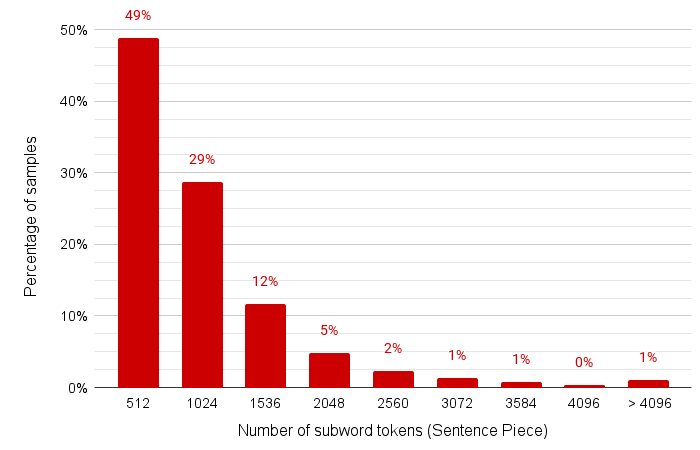
\includegraphics[width=0.8\textwidth]{Images/ivacic.samples_tokens_hist.png}
  \caption{Subword token distribution across all samples in the $NewsMon$.}
  \label{fig:tokens_hist}
\end{figure}

Binary cross-entropy (BCE) loss~\citep{goodfellow2016deep} with sigmoid activation is a standard baseline for multi-label classification, where each label is treated as an independent binary prediction. 
% Maybe skip this loss function study
However, BCE struggles with label imbalance and dependencies, prompting the use of alternative loss functions. 
Focal Loss~\citep{lin2017focal} emphasises hard-to-classify instances, while Class-Balanced Loss (CB)~\citep{cui2019classbalanced} re-weights classes based on their effective instance count. 
Distribution-Balanced Loss~\citep{wu2020distributionbalanced} mitigates label co-occurrence redundancy and applies Negative Tolerant Regularisation (NTR) to down-weight easy negative labels. 
CB-NTR Loss~\citep{huang2021balancing} integrates CB and NTR for improved balance, and~\citep{fallah2023exploitinglabeldependencies} introduces a regularisation term based on label co-occurrence and output~activations.

In addition to incorporating label co-occurrence and imbalances into the loss function computation, contrastive learning techniques have gained popularity in specific multi-label classification tasks~\citep{piskorski-etal-2023-semeval-task3}. 
For multi-label text classification, these methods often calculate a combined loss that includes both binary cross-entropy and contrastive loss~\citep{liao2023marseclipse, reiterhaas2023mcpt}. 
Interestingly, we encountered similar techniques widely used in computer vision~\citep{tunstall2022efficient, zheng-etal-2022-contrastive}, which are also predominant in learning dense document representations for dense retrievers in IR systems~\citep{reimers-2019-sentence-bert, zhang2024mgte, sturua2024jinaembeddingsv3multilingualembeddingstask, chen2024bgem3embeddingmultilingualmultifunctionality}.
A common technique for improving IR-based MLC/XMC systems utilises contrastive loss with in-batch negative sampling~\citep{dahiya2023ngame} and even incorporates label semantics into neural network architectures by combining document and label representations~\citep{you2019attentionxmllabeltreebasedattentionaware, chang2020tamingpretrainedtransformersextreme, jiang2021lightxmltransformerdynamicnegative}.
These methods differ in their use of sparse or dense label representations and whether they employ the same or different encoders for labels and documents. 
For example, the~XMC X-Transformer model utilises sparse label representations with Label Semantic Indexing, which aids in clustering labels and enhances classification performance~\citep{chang2020tamingpretrainedtransformersextreme}. 
The DEPL model~\citep{zhang2023longtailed} recently enhanced tail label prediction over X-Transformer by using sparse representations to generate pseudo descriptions, which are processed by the same encoder as documents. 
These and similar dual encoder (DE) models, which extend InfoNCE~\citep{oord2019representationlearningcontrastivepredictive} contrastive loss, improve memorisation, and~can generalise for unseen queries, are recent SOTA approaches in XMC~\citep{gupta2024dexml}.
However, a~similar approach is employed in the RAE-XMC~\citep{wang2025retrievalaugmentedencodersextrememultilabel} framework, which does not require training end-to-end for~prediction.

Research in low-resource NLP for large-scale multi-label text classification remains scarce, with~most existing work focusing on tasks involving a limited number of classes, such as sentiment analysis, hate speech detection, or~identification of sexist content~\citep{magueresse2020lowresourcelanguagesreviewpast, pakray2025lowresourcenlp}.

%%%%%%%%%%%%%%%%%%%%%%%%%%%%%%%%%%%%%%%%%%
\section{Data~Description}
\label{sec:data_description}


\subsection{Data~Preparation}
\label{sec:data_preparation}

The overall news monitoring archive contains over 85 million articles marked with more than 96,000 arbitrary ``client topics.'' To make the problem tractable and ensure a diverse representation of the language used in news media, we sampled articles from a news monitoring archive spanning January 2023 to December 2023. The~sampled NewsMon dataset comprises one million articles from eight countries (Serbia, Slovenia, Bosnia and Herzegovina, Croatia, North Macedonia, Montenegro, Kosovo, and~Albania) in nine languages (see Figure~\ref{fig:languages_hist}).
\vspace{-3pt}
\begin{figure}[H]
 % \centering
  %\subfloat[\centering]{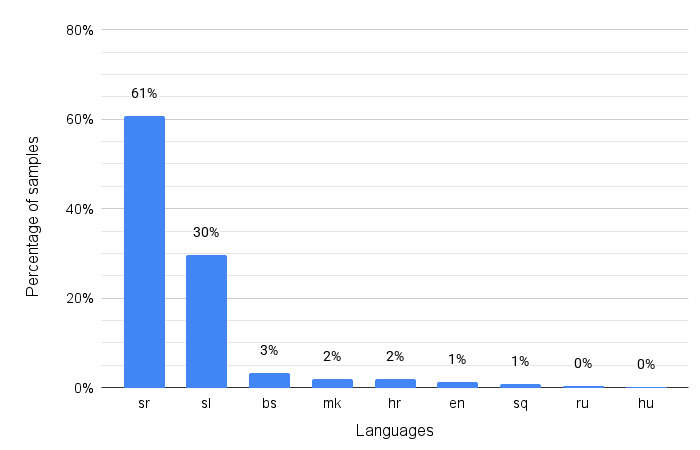
\includegraphics[width=0.49\textwidth]{Images/ivacic.samples_lang_hist.png}}
  %\subfloat[\centering]{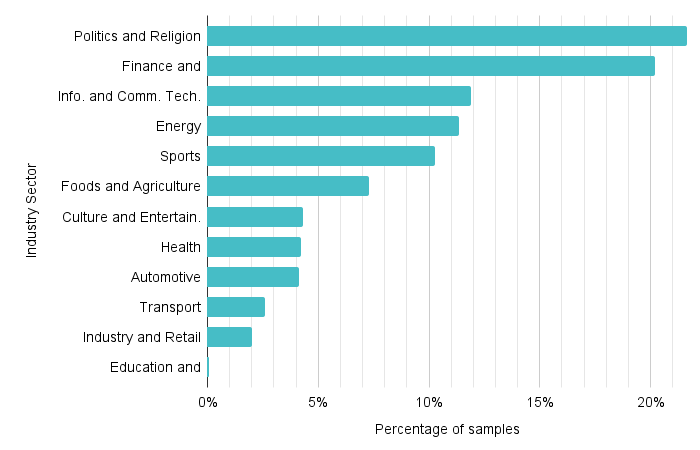
\includegraphics[width=0.51\textwidth]{Images/ivacic.sectors_samples.png}}
  %\caption{(\textbf{a}) The distribution of languages in all samples (Serbian, Slovene, Bosnian, Macedonian, Croatian, English, Albanian, Russian and Hungarian. (\textbf{b}) The distribution of Selected Industry Sector Labels across all samples.}
  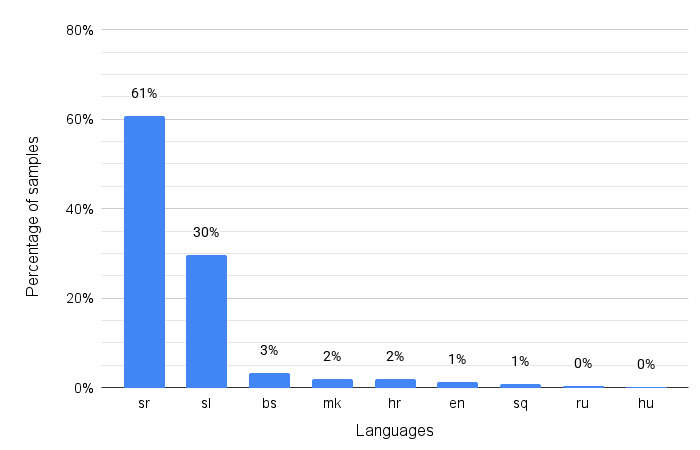
\includegraphics[width=0.9\textwidth]{Images/ivacic.samples_lang_hist.png}
  \caption{The distribution of languages in all samples (Serbian, Slovene, Bosnian, Macedonian, Croatian, English, Albanian, Russian and~Hungarian.}
  \label{fig:languages_hist}
\end{figure}



The selection process was guided by the labels corresponding to various industry sectors, enabling broad coverage of sector-specific news (see Figure~\ref{fig:sectors}).
The dataset is annotated with more than twelve thousand distinct labels. 
It encompasses all labels tracked by the monitoring system, not just those from the selected industries used for the initial~selection.

\begin{figure}[H]
%  \centering
  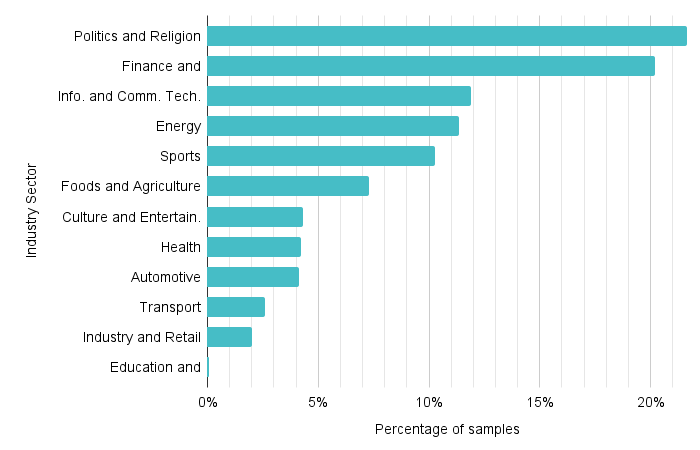
\includegraphics[width=0.70\textwidth]{Images/ivacic.sectors_samples.png}
  \caption{The distribution of selected industry sector labels across all~samples.}
  \label{fig:sectors}
\end{figure}

Each article is assigned labels representing concepts or ``topics of interest'' to clients.
Despite the system's vast number of labels, each client typically monitors only a few.
Each label is associated with several simplified keyword Boolean expressions (KwEs) that determine the initial assignment of labels to news articles (see Table~\ref{tab:kwes}).

%\renewcommand{\arraystretch}{1.1}
\begin{table}[H]
    \small
    \caption{Examples of simplified Keyword-Boolean Expressions.}
   % \setlength{\tabcolsep}{3pt}
    %\resizebox{0.75\textwidth}{!}{
   
\begin{adjustwidth}{-\extralength}{0cm}
%\centering %% If there is a figure in wide page, please release command \centering
%MDPI: Please check if hyphen format in this table is correct or not.
%MDPI: Please add explanation for * in Table footer.
%AUTHORS: fixed hypens and added a note.
 \begin{tabularx}{\fulllength}{lL}
        \toprule
        \textbf{Keyword Expression}& \textbf{Explanation}\\
        \midrule
        \mbox{tesla OR teslo OR tesli OR } \mbox{tesle --``nikol* tesl*''} & Match the Tesla car brand if Nikola Tesla the person-phrase is not present in text\\
        \midrule
        \mbox{mercedes* --formul*} \mbox{--``max verstap*'' --F1 \dots} & Match the Mercedes car brand if Formula 1 terms and phrases are absent.\\
        \midrule
        \mbox{nlb* --``lig* nlb'' --``nlb lig*''} & Match all forms of NLB terms, but~only if the NLB-sponsored league phrases are not present. (NLB is an acronym for the company Nova Ljubljanska Banka)\\
        \midrule
        \mbox{gradnj* --cest* --avtocest*} \mbox{--obvoznic*}& Match the term construction without the terms: road, highway or ring road\\
        \midrule
        \mbox{``\foreignlanguage{russian}{сенад* софтић*}'' OR} \mbox{``senad* softić*''} & Match the person-phrase with various inflections and in various scripts\\
        \bottomrule
    \end{tabularx}
\end{adjustwidth}
  %  }
  \footnotesize {\textbf{Note:} The operator \textbf{OR} denotes a logical disjunction (any listed term). The minus sign (\textbf{--}) indicates negation (exclusion). Quotation marks (``~'') define an exact phrase, and the asterisk (\textbf{*}) functions as a wildcard for variable character/sub-string endings.}
    \label{tab:kwes}
\end{table}
%AUTHORS: We introduced new \textbf{OR}, \textbf{--}, \textbf{*}. Editors can remove boldface if they wish; they can edit a note as they desire, as long as the message remains the same.
%AUTHORS: \textbf{Note:} is highlighted in all tables, but no reason is given. We confirm boldface or the word "Note:" CAN BE REMOVED IN ALL tables if editors want to do so.

News articles are automatically labelled according to those KwEs, with~additional filtering applied based on article metadata such as country, programme, section, and~media outlet.
In the final stage of the acquisition processing pipeline, a~human moderator reviews the labels assigned to each article, as~illustrated in Figure~\ref{fig:monitoring_pipeline}.
The moderator may confirm, reject, or~add additional labels based on their assessment.
The labels and their corresponding KwEs are updated whenever a new client joins or leaves, or~when a client's interests change.
These updates can occur frequently, with~about one hundred monthly label changes on average.
Arbitrary labels are also added later by the news media analysis~department.

\begin{figure}[H]
%  \centering
  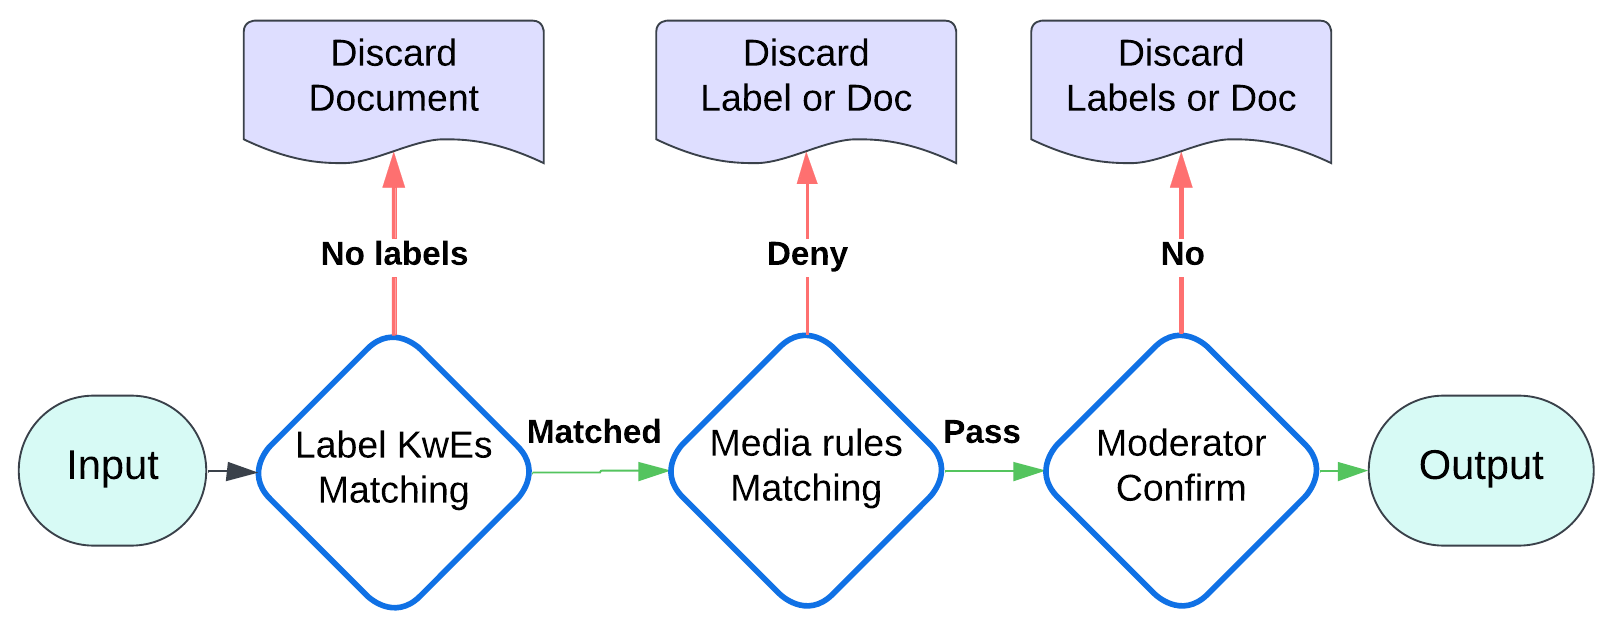
\includegraphics[width=0.70\textwidth]{Images/ivacic.monitoring_pipeline.png}
  \caption{Decision flow of the news monitoring acquisition processing pipeline. Each stage applies progressive filtering and finally human moderation to remove irrelevant data before output.}
  \label{fig:monitoring_pipeline}
\end{figure}

Upon further examination, we observed that the labels fall into two broad~classes:
\begin{itemize}\itemsep=0pt
  \item Named Entities (NE): %MDPI: Please confirm if the bold is unnecessary and can be removed. The following highlights are the same.
  %AUTHORS: We confirm boldface can be removed. 
 mostly Persons, Organisations, Products, Brands and\linebreak rarely Locations.
  \item General Concepts (GC): a set of terms representing a concept, for~example E-Mobility, Health insurance, Climate change, and Industrial waste.
\end{itemize}

We also found numerous labels with KwEs, most often from the NE class, that would match the same text.
These duplicates could potentially be removed or the classification process optimised for the NE class of labels.
However, we deliberately chose not to apply such interventions to evaluate the robustness of our methods in real-world applications, thereby avoiding the introduction of additional and potentially brittle label-cleaning pipelines.
Some labels, especially those of the GC class, are often context-dependent. 
For example, while the ``Competition'' label applies to many industries and may seem like a duplicate, its meaning and KwEs vary depending on the context and client.
Moreover, we observed that label sets are distinct across different languages in our setting, with~limited overlap in their semantic or structural alignment, making cross-lingual analysis unlikely to yield meaningful performance~benefits.

For data preparation, we first identified and removed duplicate or near-duplicate samples, which accounted for 18\% of the dataset. 
These duplicates primarily originated from news aggregators, copied press releases, and~other replicated content. 
Although such duplication is valuable in the news monitoring industry for assessing media reach, it was necessary to eliminate it for our classification task. 
Additionally, we refined the text data by extracting possible titles or metadata-polluted bodies and merging article titles with their respective body text to create a complete representation of each news~article. 

Due to the large dataset and label set size, we decided to downsample the NewsMon data. To~speed up our research cycle for testing various classification methods and techniques, we selected the Slovene subset NewsMon\textsubscript{sl}, which was chosen because it contains the largest number of distinct labels among all available language-specific subsets (see Figure~\ref{fig:label_lang_hist}).
We focused exclusively on publicly available Slovene data, as~the label sets in our dataset are distinct across languages. 
To ensure relevance and consistency with established benchmarks, we selected data from January 2023 to May 2023, targeting a dataset size and label distribution comparable to well-known multi-label datasets.
We removed labels that appeared only once to prepare the dataset for training. 
Finally, we applied uniform random sampling to partition the dataset into training (80\%), validation (10\%), and~test (10\%) sets.
Before sampling, the~dataset was shuffled to minimise the potential impact of temporal label dynamics; however, some bias in evaluation may still be present due to a long-tail~distribution.

\begin{figure}[H]
%  \centering
  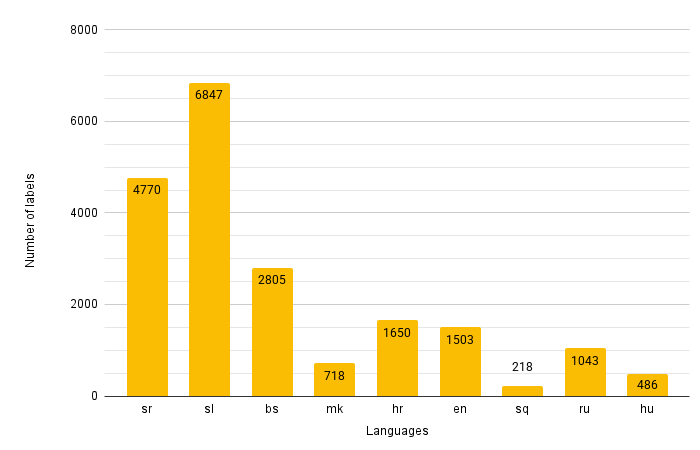
\includegraphics[width=0.70\textwidth]{Images/ivacic.labels_lang_hist.png}
  \caption{The distribution of labels per language (Serbian, Slovene, Bosnian, Macedonian, Croatian, English, Albanian, Russian and Hungarian).}
  \label{fig:label_lang_hist}
\end{figure}


\subsection{Data~Analysis}

For comparison, we selected the EURLEX57K dataset~\citep{chalkidis-etal-2019-large}, commonly referred to as EURLex-4.3K in XMC, as~it is a widely used large-scale multi-label text classification dataset with label and instance sizes similar to those of our down-sampled version. 
More importantly, this comparison enables us to assess the performance of our classifiers in Section~\ref{sec:methods}. 
We adopt some of the EURLEX57K evaluation metrics to evaluate model effectiveness, examining how the same models perform when trained on our dataset, which consists of a lesser-used language in the model pre-training. 
We first introduce label distribution metrics to facilitate this analysis before exploring the similarities and differences between the two datasets.
Both datasets, NewsMon\textsubscript{sl} and \mbox{EURLEX57K}, exhibit a long-tail label distribution, where most labels occur infrequently. 
%\renewcommand{\arraystretch}{1.3}


The NewsMon\textsubscript{sl} dataset comprises 50,784 instances and 3,231 labels, with~an average of 2.99 labels per instance. 
The label density is 0.00093, indicating that labels are distributed sparsely across the dataset.
Since we removed single-occurring labels, this results in a slightly lower average of labels per instance but a higher label density, reflecting a more concentrated label distribution after filtering (see Table~\ref{tab:dataset_statistics}). Definitions of label distribution metrics are explained in Appendix~\ref{sec:label_distribution_metrics}.

\begin{table}[H]
    \centering
    \caption{Dataset statistics for the complete set (NewsMon), selected initial set of labels (NewsMon\textsubscript{initial}), the~down-sampled dataset in Slovene (NewsMon\textsubscript{sl+dups}) with all labels, and~the down-sampled dataset with single-occurrence labels and duplicates removed (NewsMon\textsubscript{sl}). }
  %  \resizebox{0.75\textwidth}{!}{
        \begin{tabularx}{\textwidth}{lcCcCc}
            \toprule
            \textbf{Dataset} & \textbf{Samples} & \textbf{Labels} & \textbf{Cardinality} & \textbf{Density} & \textbf{Diversity} \\
            \midrule
         
            NewsMon & 1,068,261 & 12,305 & 3.392 ± 4.017 & 0.00028 & 267,564 \\
            NewsMon\textsubscript{initial} & 1,068,261 & 1960 & 2.213 ± 2.316 & 0.00114 & 183,361 \\
            NewsMon\textsubscript{sl+dups} & 62,049 & 4052 & 3.034 ± 3.492 & 0.00075 & 17,307 \\
            NewsMon\textsubscript{sl}& 50,784 & 3231 & 2.995 ± 3.463 & 0.00093 & 15,809 \\
            \midrule
            EURLEX57K & 57,000 & 4271 & 5.069 ± 1.701 & 0.00119 & 34,982 \\
            \bottomrule
        \end{tabularx}
  %  }
    \label{tab:dataset_statistics}
\end{table}


The EURLEX57K dataset, with~57,000 instances and 4,271 labels, has an average of 5.07 labels per instance and a label diversity of 35,000, indicating a more challenging label space compared to the NewsMon\textsubscript{sl} dataset.
A high standard deviation for cardinality in NewsMon\textsubscript{sl} datasets suggests that the number of labels per instance is spread over a broader range.
Overall, the~datasets exhibit similar properties regarding the long-tail label distribution, as~illustrated in \cref{fig:filtered_articles,fig:eurlex}.
\vspace{-3pt}
\begin{figure}[H]
%  \centering
 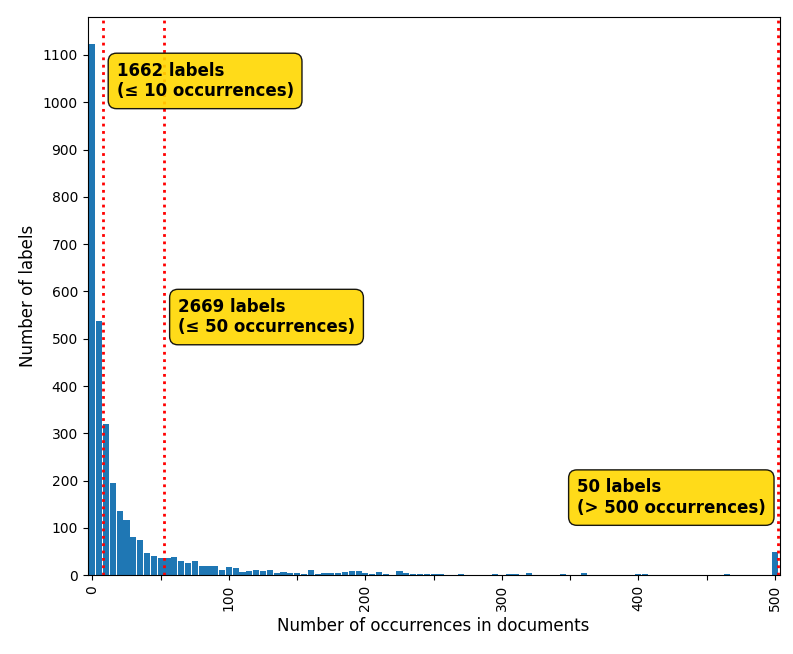
\includegraphics[width=0.65\textwidth]{Images/ivacic.label_dist_newsmon_sl-2.png}
  \caption{The distribution of label occurrences in the NewsMon\textsubscript{sl} dataset.}
  \label{fig:filtered_articles}
\end{figure}
\vspace{-6pt}

\begin{figure}[H]
%  \centering
  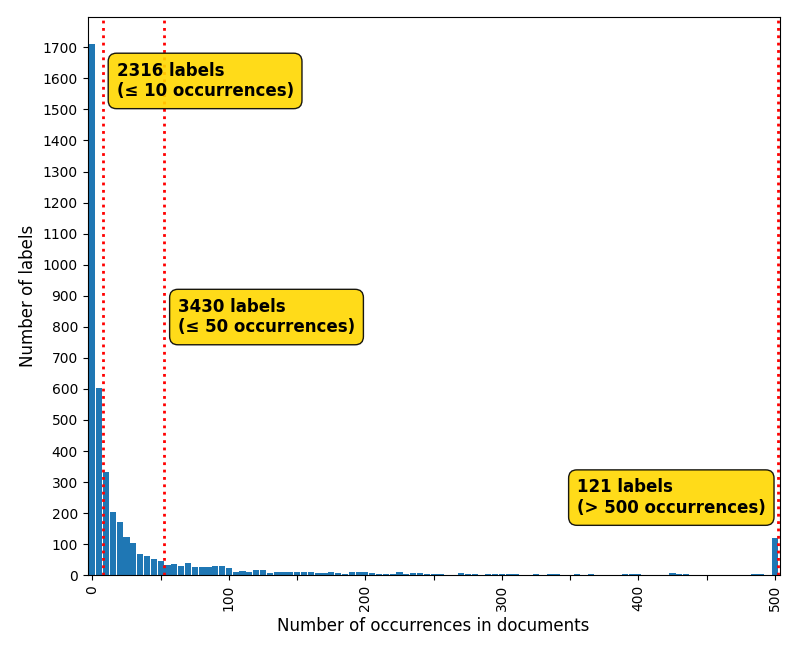
\includegraphics[width=0.65\textwidth]{Images/ivacic.label_dist_eurlex57k-2.png}
  \caption{The distribution of label occurrences in the EURLEX57K~dataset.}
  \label{fig:eurlex}
\end{figure}

We applied Uniform Manifold Approximation and Projection (UMAP) to visualise the label space of the dimensionality-reduced training sets for each dataset separately (Figures~\ref{fig:umap_newsmon} and~\ref{fig:umap_eurlex}). 
While not intended for direct comparison, the~visualisations reveal that neither dataset exhibits a clear underlying structure or distinct clustering~patterns.


\begin{figure}[H]
%  \centering
  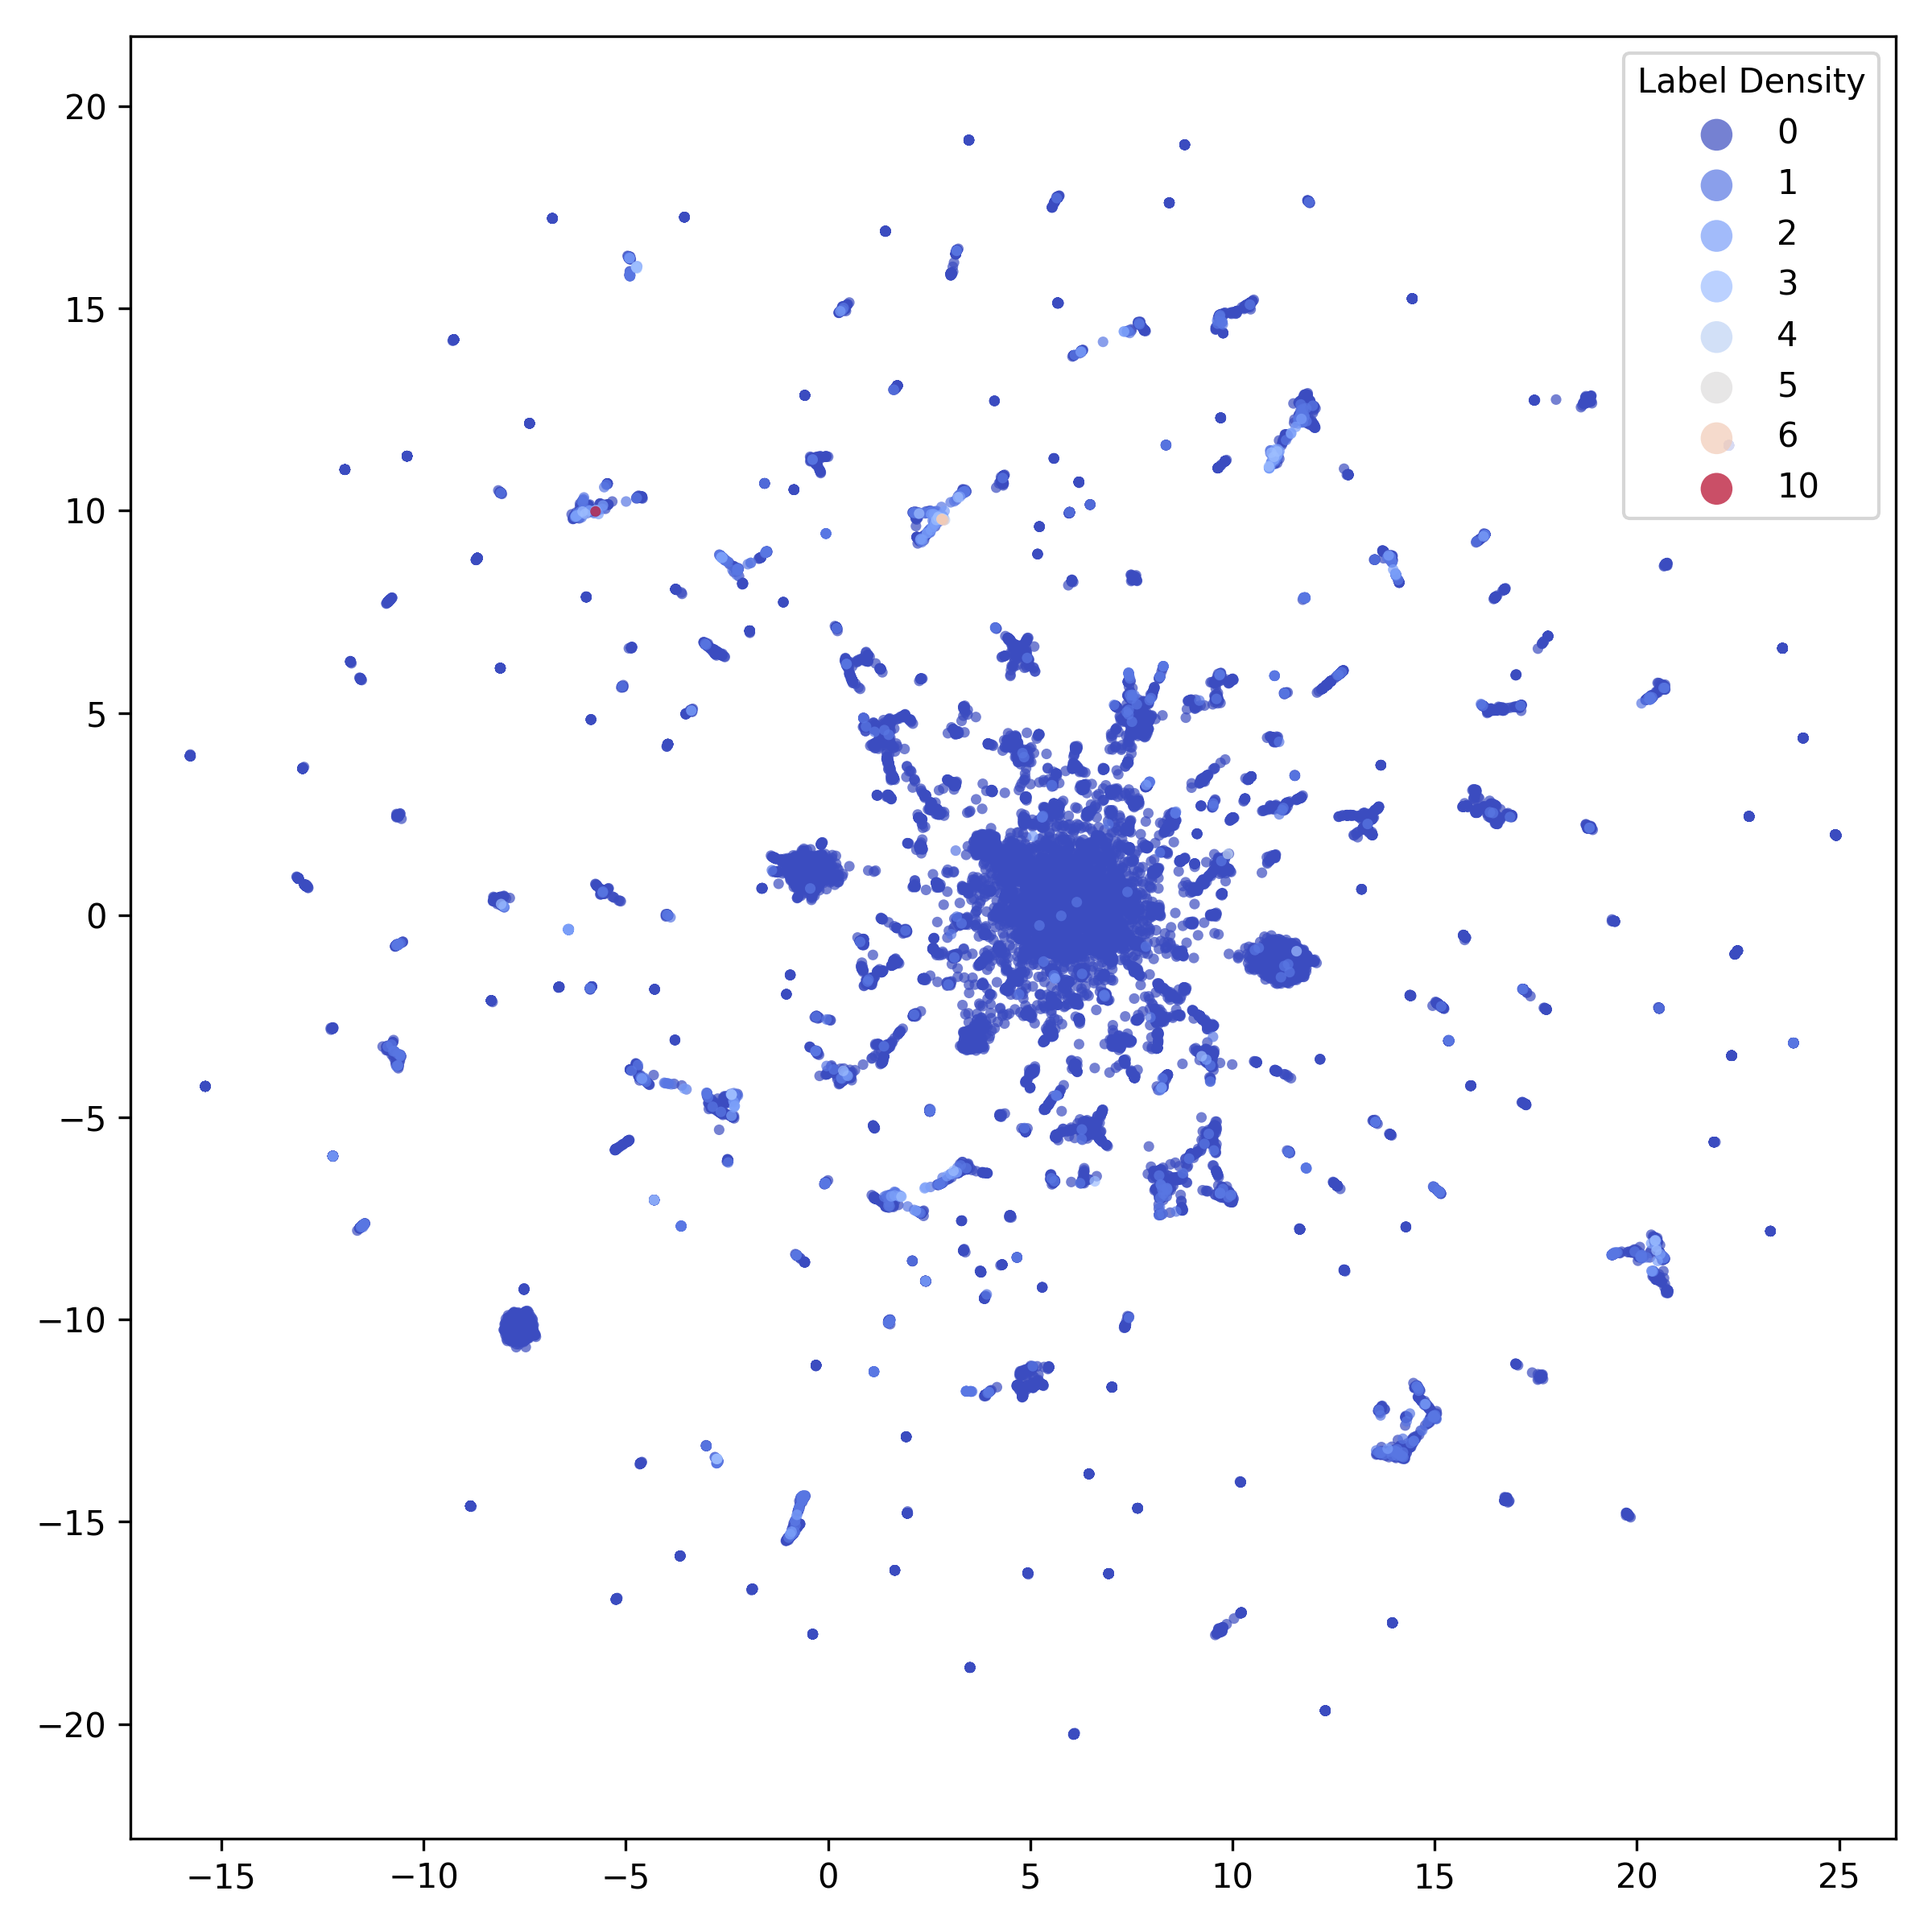
\includegraphics[width=0.8\textwidth]{Images/ivacic.label_tsne_proj2_newsmon_sl-1.png}
  \caption{UMAP visualization of the NewsMon\textsubscript{sl} dataset.}
  \label{fig:umap_newsmon}
\end{figure}
\vspace{-6pt}

\begin{figure}[H]
%  \centering
  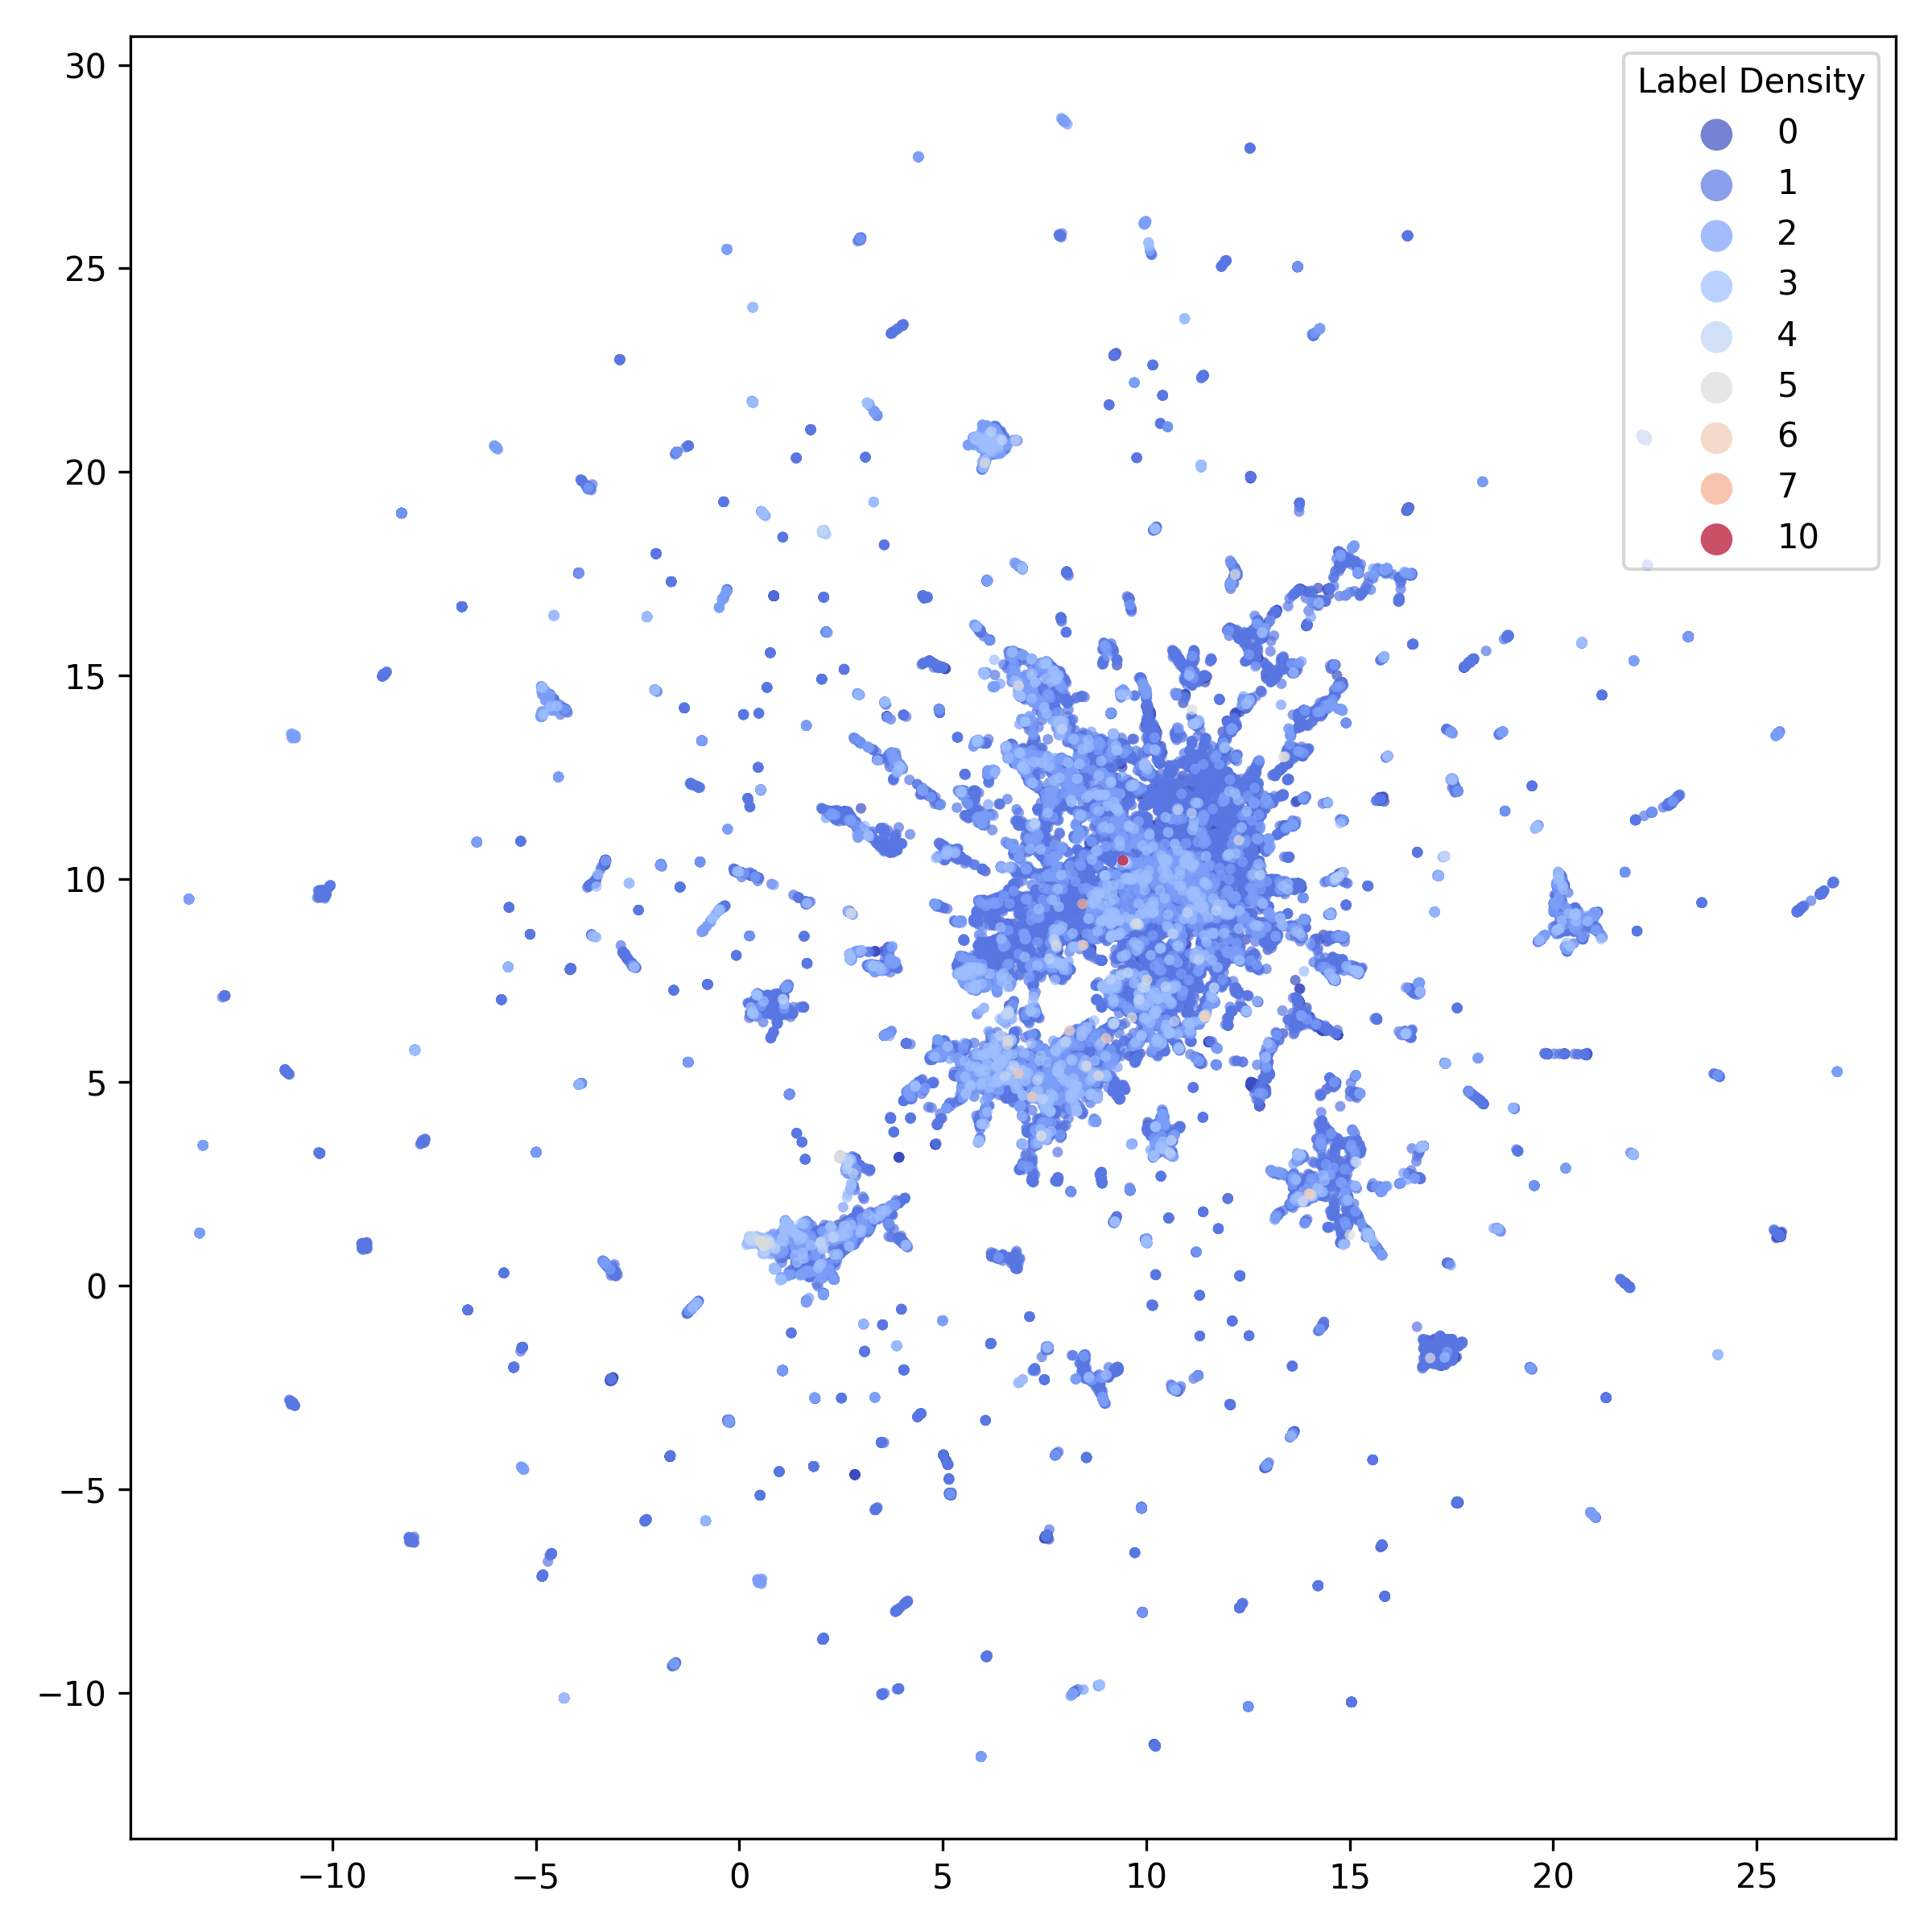
\includegraphics[width=0.8\textwidth]{Images/ivacic.label_tsne_proj2_eurlex-1.png}
  \caption{UMAP visualization of the EURLEX57K~dataset.}
  \label{fig:umap_eurlex}
\end{figure}

%%%%%%%%%%%%%%%%%%%%%%%%%%%%%%%%%%%%%%%%%%
\section{Methodology}
\label{sec:methods}



The proposed methodology is presented in Figure~\ref{fig:method}. In~summary, compared to the original methodology, shown in Figure~\ref{fig:rae_xmc_framework} of Appendix~\ref{sec:raexmc_model}, we have added IR model fine-tuning using hard negatives and did not use label descriptions, as~they were not~available.
\begin{figure}[H]
%  \centering
  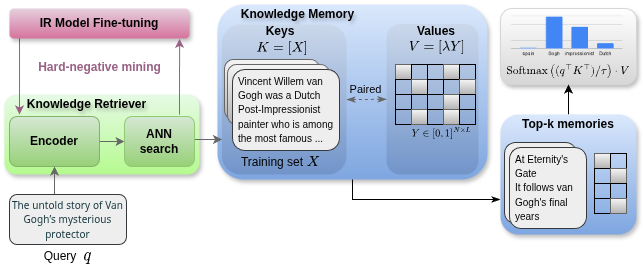
\includegraphics[width=1.0\textwidth]{Images/ivacic.raexmc_simpl_model.png}
  \caption{The proposed methodology based on~RAE-XMC (adapted from~\citep{wang2025retrievalaugmentedencodersextrememultilabel}).}
  \label{fig:method}
\end{figure}
The methodology is explained in detail below.
We built on the idea of the RAE-XMC framework initially presented in~\citep{wang2025retrievalaugmentedencodersextrememultilabel}, which decomposes $p(y_{\ell} | q)$, the~conditional probability of label $\ell$ being relevant to a test input $q$, into~retrieval from knowledge memory $K$ and prediction conditioned on the retrieved key $k$ and test input $q$. 
Therefore, given the test input $q$, retrieve relevant keys $k$ from a knowledge memory $K$, and~then use the predictive score for label $y_{\ell}$ to predict the sample label set. The~method decomposes the classification process to sampling from the retriever distribution $p(k | q; \theta)$ and predictive score $p(y_{\ell} | k, q)$:
\begin{equation}
p(y_\ell \mid q) = \sum_{k \in \mathcal{K}} 
\underbrace{p(y_\ell \mid k, q)}_{\text{Predictor}} \cdot 
\underbrace{p(k \mid q; \theta)}_{\text{Retriever}}.
\end{equation}

The knowledge memory $K$ consists of training instances $X$ and label descriptions $Z$ each paired with label values $V$, where 
$V$ matrix is composed of training ground truth $Y$ label values and an identity $I$ matrix representing ground truth for each label description:
\begin{equation}
K = 
\begin{bmatrix}
x_1^\top, \ldots, x_N^\top, z_1^\top, \ldots, z_L^\top
\end{bmatrix} 
= 
\begin{bmatrix}
X, Z
\end{bmatrix} 
\in \mathbb{R}^{(N+L) \times d} ,
\end{equation}
\begin{equation}
V = 
\begin{bmatrix}
\lambda Y, (1-\lambda) I_L
\end{bmatrix} 
\in [0, 1]^{(N+L) \times L} .
\end{equation}

The retriever is then defined as:
\begin{equation}
p(k | q; \theta) = \frac{\exp(s_{\theta}(q, k)/\tau)}{\sum_{k' \in K} \exp(s_{\theta}(q, k')/\tau)} \sim \text{Softmax}((q^{\top}K^{\top})/\tau),
\end{equation}
and predictor as a simple label lookup:
\begin{equation}
p(y_{\ell} | k, q) = V_{k, \ell} \in \{0, 1\},
\end{equation}
where the underlying scorer is a dense embedding-based model $s_{\theta}(k, q) = \langle f_{\theta}(k), f_{\theta}(q) \rangle$ which outputs $d$-dimensional embeddings, and~$\tau$ is the temperature controlling the skewness of the Softmax~distribution.

Our datasets lack label descriptions, and~initial experiments with synthetically generated pseudo-descriptions, similar to DEPL~\citep{zhang2023longtailed}, produced suboptimal results. 
Consequently, we opted to simplify the model and conduct our experiments without label pseudo-descriptions.
Therefore, our knowledge memory is simplified to:
\begin{equation}
K = 
\begin{bmatrix}
x_1^\top, \ldots, x_N^\top
\end{bmatrix} 
= 
\begin{bmatrix}
X
\end{bmatrix} 
\in \mathbb{R}^{N \times d},
\end{equation}
where the ground-truth label values are:
\begin{equation}
V = 
\begin{bmatrix}
\lambda Y
\end{bmatrix} 
\in [0, 1]^{N \times L}.
\end{equation}

We retained the $\lambda$ hyperparameter and reformulated the simplified model in matrix form as follows:
\begin{equation}
\hat{p} = \text{Softmax}\left((q^{\top}K^{\top})/\tau\right) \cdot \lambda Y \in \mathbb{R}^{1 \times L}.
\end{equation}

For embedding and similarity search, we employed the best-performing pre-trained IR model from our zero-shot experiments (see Section~\ref{sec:experiments}), which we further fine-tuned using hard negatives.
The selected pre-trained retrieval model encodes the input query $q$ into a sequence of hidden states $H_q$ using a text encoder. The~query representation is obtained by applying layer normalisation to the hidden state corresponding to the special ``[CLS]'' token of the Transformer Encoder:
\begin{equation}
f_{\theta}(q) = \text{norm}(H_q[0]).
\end{equation}

Similarly, a~key $k$ (training document) is encoded to produce hidden states $H_k$, and~its representation is obtained as:
\begin{equation}
f_{\theta}(k) = \text{norm}(H_k[0]),
\end{equation}
applying the layer normalisation:
\begin{equation}
\text{norm}(x) = \gamma \cdot \frac{x - \mu}{\sqrt{\sigma^2 + \epsilon}} + \beta,
\end{equation}
where $\mu$ is the mean of the vector $x \in \mathbb{R}^d$ (the [CLS] hidden state), $\sigma^2$ is the variance, $\epsilon$ is a small stability constant and $\beta, \gamma \in \mathbb{R}^d$ are learnable scale and shift~parameters.

The relevance between the query and the key is then computed as the inner product of their embeddings.
We performed further retrieval optimisation with hard negative (HN) mining, inspired by the approach outlined in~\citep{xiong2021ance}, to~be used in conjunction with contrastive~learning.

Specifically, we embedded all training samples using the same encoder and identified the closest samples that did not share labels as hard negatives. 
We operate under a fixed negative budget of at most 15 in-batch negatives per query due to memory constraints during training.
Therefore, for~each training query $q$, we selected up to 15 negative keys $k \in K'$ that maximise the total similarity:
\begin{equation}
K' = \underset{S \subseteq K,\, |S| = 15}{\operatorname{argmax}} \sum_{k \in S} s_\theta(q, k), \quad \text{subject to } y_q \cap y_k = \emptyset
\end{equation}
and one positive key:
\begin{equation}
k^* = \underset{k \in K}{\operatorname{argmax}}\, s_\theta(q, k), \quad \text{subject to } y_q \cap y_k \neq \emptyset
\end{equation}
where $q, k \in K$ and their corresponding label sets $y_q, y_k \in V$.

The training process was optimised using the same contrastive \mbox{InfoNCE} loss as in pre-training, formally defined by the following loss function:
\begin{equation}
\mathcal{L}_{\operatorname{InfoNCE}}(\cdot) = - \log \left( \frac{\exp(s_{\theta}(q, k^*)/\tau)}{\sum_{k \in \{k^*, K'\}} \exp(s_{\theta}(q, k)/\tau)} \right),
\end{equation}
where $k^*$ and $K'$ are the positive and negative samples to the query $q$; $s_{\theta}(p, k) = \langle f_{\theta}(k), f_{\theta}(q) \rangle$ is a scoring function of the query and sample dense embeddings $f_{\theta}$.

Lastly, our approach leveraged multi-objective genetic algorithm hyperparameter optimisation through the Optuna framework~\citep{akiba2019optunanextgenerationhyperparameteroptimization}, which provides superior efficiency compared to traditional grid search methods.
The hyperparameter search space encompassed critical parameters including retriever temperature $\tau$, weighting factor $top\mhyphen k$ and $\lambda$, predictor values, with~subset accuracy serving as the optimisation objective across 1000 trials (see Appendix~\ref{subsec:hyper_parameter_search} for details).

Algorithm~\ref{alg:rae-xmc-python} summarises our test-time procedure for the simplified RAE-XMC variant. 
Given an input text $q$, we encode it with the hard-negative–fine-tuned retriever, retrieve the $top\mhyphen k$ nearest training instances from the index, and~convert their similarity scores into weights via a temperature-scaled Softmax with parameter $\tau$. 
These weights linearly combine the pre-scaled label matrix $V=\lambda \cdot Y$ to yield class probabilities, which are then thresholded to produce the final label set. 
Unless otherwise noted, $k$, $\tau$, and~the decision threshold are fixed to the values selected during hyperparameter search.
\begin{algorithm}[H]
\caption{Modified RAE-XMC~Inference}
\label{alg:rae-xmc-python}
\begin{algorithmic}[1]
\State \textbf{Example hyperparameters (illustrative):} $top\mhyphen k \gets 50$, threshold $\gets 0.5$, $\tau\gets 0.04$
\State \textbf{Pre-scale values:} $V \gets \lambda \cdot Y$
\Function{RAEXMC\_Mod} {$q$, hn\_encoder, index, V, $top\mhyphen k$, $\tau$, threshold}
  \State embedding $\gets$ hn\_encoder($q$)
  \State K\_matches $\gets$ index(embedding, $top\mhyphen k$)
  \State $\alpha \gets $ softmax(K\_matches$/\tau$)
  \State probabilities $\gets \alpha \cdot V$
  \State \Return (probabilities $>$ threshold)
\EndFunction
\end{algorithmic}
\end{algorithm}



%%%%%%%%%%%%%%%%%%%%%%%%%%%%%%%%%%%%%%%%%%
\section{Experimental~Setting}
\label{sec:experiments}

For the initial set of experiments, which tested traditional methods, we used a term frequency–inverse document frequency (TF-IDF) representation in combination with one-versus-all (OVA) classifiers, specifically Support Vector Machines~\citep{cortes1995support} (SVM) and Logistic Regression~\citep{cox58reg}.
For both models, we used grid search~\citep{scikit-learn} to obtain the best-performing hyperparameters (see Appendix~\ref{sec:hyper_parameters} for details).

As a baseline, we trained the XLM-RoBERTa-base~\citep{conneau2019xlmr} model five times with different random seeds using binary cross-entropy (BCE) loss and a standard classification head, which produces a probability per label.
For the baseline training, we used a standard set of hyperparameters (see Appendix~\ref{sec:hyper_parameters} for details), without~performing any hyperparameter optimisation, as~our results (0.760 micro-averaged F1-score) exceeded the best reported performance (0.732) by the original EURLEX57K authors~\citep{chalkidis-etal-2019-large}.

To compare to classical k-Nearest Neighbours (KNN) approaches, we selected the ML-KNN algorithm~\citep{zhang2007mlknn}. 
The ML-KNN algorithm leverages the KNN approach to classify instances in a multi-label setting by combining neighbour-based similarity with Bayesian inference. 
First, it identifies the k nearest neighbours of a given data point using a predefined distance metric, typically Euclidean distance. 
Then, it applies Bayesian inference to estimate the probability of each label being relevant to the test instance based on the labels of its k nearest neighbours. 
Finally, the~algorithm utilises the Maximum a posteriori (MAP) principle to determine the most likely set of labels for the unseen instance, considering the distribution of labels among its nearest neighbours. 
For all experiments, we employed Faiss's~\citep{johnson2019billion,douze2024faiss} graph-based Approximate Nearest Neighbour (ANN) Hierarchical Navigable Small World (HNSW) algorithm for KNN search.
Samples were classified as positive when their predicted probability exceeded a threshold of~0.5.

When the focus is strictly on pre-trained information retrieval (IR) models, computational efficiency is closely tied to both the architecture and the task-specific tuning present at deployment. 
Most Small Language Models (SLMs) available today, such as those benchmarked by~\citep{lu2025smalllanguagemodelssurvey}, are generalist language models with optional support for retrieval, question-answering, or~in-context learning. 
However, very few are distributed with explicit, out-of-the-box pre-training for dense or hybrid multilingual~IR.

To identify the most effective IR model and assess the feasibility of our approach, we conducted zero-shot experiments. 
In these experiments, we embedded the training set and classified labels based on the labels of the nearest neighbour. 
To mitigate the truncation issue discussed in Section~\ref{sec:related_work}, in~these experiments, we selected three competitive multilingual retrieval models capable of processing extended contexts of up to 8000 subword tokens, listed below:

\begin{itemize}\itemsep=0pt
  \item Alibaba-NLP/gte-multilingual-base (GTE-mb)~\citep{zhang2024mgte};
  \item jinaai/jina-embeddings-v3 (Jina-v3)~\citep{sturua2024jinaembeddingsv3multilingualembeddingstask};
  \item BAAI/bge-m3 (BGE-M3)~\citep{chen2024bgem3embeddingmultilingualmultifunctionality}.
\end{itemize}

The selected model specifications are outlined in Table~\ref{tab:model_specs}.
\begin{table}[H]
    
    \caption{Best multilingual IR model specifications including supported token count, embedding dimension, parameter size, memory usage, and~MTEB ranking metrics for multilingual (ML) and English (EN) tasks.}
    %\resizebox{0.65\textwidth}{!}{
    %\setlength{\tabcolsep}{6pt} % adjusts column spacing for readability
    \begin{tabularx}{\textwidth}{l C c C c C c}
        \toprule
        \multicolumn{1}{c}{\textbf{Model}} &
        \multicolumn{1}{c}{\textbf{Tokens}} &
        \multicolumn{1}{c}{\textbf{Dim}} &
        \multicolumn{1}{c}{\textbf{Params [M]}} &
        \multicolumn{1}{c}{\textbf{Mem [MB]}} &
        \multicolumn{1}{c}{\textbf{ML}} &
        \multicolumn{1}{c}{\textbf{EN}} \\
        \midrule
        
        GTE-mb  & 8192 & 768  & 305 & 582  & 6 & 31 \\
        Jina-v3 & 8194 & 1024 & 572 & 1092 & 8 & 7  \\
        BGE-M3  & 8194 & 1024 & 568 & 2167 & 5 & 89 \\
        \bottomrule
    \end{tabularx}
   % }
    \label{tab:model_specs}
\end{table}

These models were either initialised from an XLM-RoBERTa checkpoint or trained from scratch, making them directly comparable to our main experimental baseline. 
They share a similar transformer encoder architecture and parameter count, and~undergo additional multi-stage fine-tuning for IR tasks. 
Notably, none of these models were explicitly trained on any target South Slavic~language.

According to the MTEB benchmark~\citep{enevoldsen2025mmtebmassivemultilingualtext}, these multilingual models are the top performers among sub-billion parameter language models specifically designed and pre-trained for large-scale, multilingual IR. 
They exhibit a highly efficient computational profile, requiring only approximately \(\sim\)2.6~GB of GPU memory (see Section~\ref{sec:inference-efficiency}) for inference in our experiments, which enables deployment on edge devices or targeted consumer-grade hardware~\citep{jang2025edgefirstlanguagemodelinference}.
%The operational costs for pre-trained IR models of this scale remain exceptionally low, aligning with cost per million tokens in the \$0.005–0.02 range and energy footprints below 20\% of those required by LLMs~\cite{jang2025edgefirstlanguagemodelinference}. 
This makes pre-trained IR models particularly desirable for real-world deployments with strict latency, scale, or~environmental~constraints.

In contrast, most generic small language models (SLMs) with fewer than 1 billion parameters, unless~specifically fine-tuned, tend to fall short in both text classification tasks~\citep{bucher2024finetunedsmallllmsstill, galke2025reallymakingprogresstext} and retrieval performance for practical applications~\citep{enevoldsen2025mmtebmassivemultilingualtext}.

Finally, we selected the BGE-M3 model for further experimentation, as~it demonstrated the best performance across both datasets, as~shown in Tables~\ref{tab:zero_ir_newsmonsl} and ~\ref{tab:zero_ir_eurlex}. 
The zero-shot experiments capture the lower bound of the model’s performance, representing the worst-case expected results under dynamic label space conditions; therefore, a~time-based holdout was deemed~unnecessary.
\begin{table}[H]
%    \centering
\small
    \caption{Zero-shot performance on NewsMon\textsubscript{sl}: micro/macro F1, precision, recall, and~subset accuracy across all, frequent, and~rare labels for GTE-mb, Jina-v3, and~BGE-M3.}
%    \resizebox{0.65\textwidth}{!}{
%    \setlength{\tabcolsep}{3pt} % reduces column spacing
    \begin{tabularx}{\textwidth}{L l C c C c C c C}
        \toprule
        \multicolumn{1}{c}{\textbf{Model}} &
        \multicolumn{1}{c}{\textbf{Frequency}} &
        \multicolumn{1}{c}{\(\boldsymbol{\upmu}\)\textbf{F1}} &
        \multicolumn{1}{c}{\(\boldsymbol{\upmu}\)\textbf{P}} &
        \multicolumn{1}{c}{\(\boldsymbol{\upmu}\)\textbf{R}} &
        \multicolumn{1}{c}{\textbf{F1}} &
        \multicolumn{1}{c}{\textbf{P}} &
        \multicolumn{1}{c}{\textbf{R}} &
        \multicolumn{1}{c}{\textbf{Acc}} \\
        \midrule
      
        GTE-mb   & All      & 57.44 & 55.21 & 59.86 & 27.02 & 27.38 & 29.47 & 40.02 \\
        Jina-v3  & All      & 58.55 & \textbf{56.27} & 61.03 & 27.58 & 27.87 & 30.11 & 40.94 \\
        BGE-M3   & All      & \textbf{59.04} & 55.84 & \textbf{62.62} & \textbf{28.28} & \textbf{28.12} & \textbf{31.18} & \textbf{42.58} \\
        \midrule
        GTE-mb   & Frequent & 73.99 & 76.30 & 71.81 & 70.28 & 74.18 & 67.86 & 62.79 \\
        Jina-v3  & Frequent & 74.93 & 77.23 & 72.78 & 71.20 & 74.61 & 69.00 & 64.51 \\
        BGE-M3   & Frequent & \textbf{76.41} & \textbf{78.41} & \textbf{74.51} & \textbf{72.63} & \textbf{75.67} & \textbf{70.63} & \textbf{65.77} \\
        \midrule
        GTE-mb   & Rare     & 50.59 & \textbf{72.85} & 38.75 & 13.89 & 14.75 & 13.54 & 30.75 \\
        Jina-v3  & Rare     & 50.68 & 72.24 & 39.03 & 13.90 & 14.71 & 13.73 & 30.54 \\
        BGE-M3   & Rare     & \textbf{52.59} & 71.70 & \textbf{41.53} & \textbf{14.72} & \textbf{15.52} & \textbf{14.45} & \textbf{33.12} \\
        \bottomrule
    \end{tabularx}
    %}
        \footnotesize {\textbf{Note:} Best results are shown in \textbf{bold}.}
    \label{tab:zero_ir_newsmonsl}
\end{table}
\vspace{-6pt}

\begin{table}[H]
   % \centering
\small
    \caption{Zero-shot performance on EURLEX57K: micro/macro F1, precision, recall, and~subset accuracy across all, frequent, and~rare labels for GTE-mb, Jina-v3, and~BGE-M3.}
%    \resizebox{0.65\textwidth}{!}{
%    \setlength{\tabcolsep}{3pt} % reduces column spacing
    \begin{tabularx}{\textwidth}{L l C c C c C c C}
        \toprule
        \multicolumn{1}{c}{\textbf{Model}} &
        \multicolumn{1}{c}{\textbf{Frequency}} &
        \multicolumn{1}{c}{\(\boldsymbol{\upmu}\)\textbf{F1}} &
        \multicolumn{1}{c}{\(\boldsymbol{\upmu}\)\textbf{P}} &
        \multicolumn{1}{c}{\(\boldsymbol{\upmu}\)\textbf{R}} &
        \multicolumn{1}{c}{\textbf{F1}} &
        \multicolumn{1}{c}{\textbf{P}} &
        \multicolumn{1}{c}{\textbf{R}} &
        \multicolumn{1}{c}{\textbf{Acc}} \\
        \midrule
       
        GTE-mb   & All      & 45.32 & 45.47 & 45.17 & 14.73 & 15.92 & 15.40 & 12.39 \\
        Jina-v3  & All      & 60.67 & 60.75 & 60.58 & 22.12 & 23.44 & 23.01 & 18.89 \\
        BGE-M3   & All      & \textbf{66.52} & \textbf{66.67} & \textbf{66.37} & \textbf{25.65} & \textbf{26.74} & \textbf{26.76} & \textbf{23.12} \\
        \midrule
        GTE-mb   & Frequent & 57.00 & 57.71 & 56.30 & 52.95 & 54.20 & 52.19 & 24.14 \\
        Jina-v3  & Frequent & 72.45 & 72.76 & 72.14 & 68.95 & 69.30 & 68.86 & 35.65 \\
        BGE-M3   & Frequent & \textbf{77.45} & \textbf{78.00} & \textbf{76.91} & \textbf{74.51} & \textbf{75.34} & \textbf{73.97} & \textbf{40.68} \\
        \midrule
        GTE-mb   & Rare     & 18.29 & 38.41 & 12.00 & 3.71  & 4.30  & 3.49  & 9.52  \\
        Jina-v3  & Rare     & 27.25 & 41.32 & 20.32 & 6.08  & 6.68  & 6.02  & 15.63 \\
        BGE-M3   & Rare     & \textbf{34.14} & \textbf{47.32} & \textbf{26.70} & \textbf{8.10}  & \textbf{8.81}  & \textbf{8.00}  & \textbf{20.60} \\
        \bottomrule
    \end{tabularx}
   %}
        \footnotesize {\textbf{Note:} Best results are shown in \textbf{bold}.}
    \label{tab:zero_ir_eurlex}
\end{table}

Note that in the experimental evaluation, resulting in  Tables~\ref{tab:zero_ir_newsmonsl} and \ref{tab:zero_ir_eurlex}, we conducted a series of experiments using the evaluation metrics explained in Appendix~\ref{sec:evaluation_metrics}. 
We assessed all models using a consistent data split across the entire dataset (setting `All' in column `Frequency') and separately on frequent labels (those occurring 500 times or more) and rare labels (those occurring 10 times or fewer), presented in `Frequent' and `Rare' in column `Frequency', respectively. In~summary, we can observe overall better performance in the zero-shot experiments on the NewsMon\textsubscript{sl} dataset, which we attribute to lower label diversity compared to~EURLEX57K.

Next, we conducted hard negative (HN) mining using the BGE-M3 model on both the EURLEX57K and NewsMon\textsubscript{sl} training sets, constructing HN datasets consisting of one positive sample and up to fifteen hard negative samples. 
We fine-tuned the same model on the HN dataset using the default hyperparameters of the BGE-M3 model. 
Finally, we performed a hyperparameter search on the validation set for the $\lambda$, $\tau$ and $top\mhyphen k$ \mbox{(see Appendix~\ref{sec:hyper_parameters}). }

\subsection*{Inference Efficiency (Latency \& Memory)}
\label{sec:inference-efficiency}



We quantified the runtime efficiency of our method on a single consumer-grade GPU accelerator with 16~GB of GPU memory, focusing on both device/host memory consumption, as~well as end-to-end inference latency. 
The model’s steady-state device footprint (parameters and runtime buffers) was 1147.4~MB of GPU memory. Under~load, the~smallest tested batch (batch size $=2$) reached an average peak of 2645.0~MB on the GPU, whereas the largest batch that fit on the device (batch size $=384$) drove the maximum allocated GPU memory for the process to 7578.7~MB. 
On the host, the~process memory peaked at an average of 2940.6~MB, where the indexed ``knowledge memory'' consumed 748.5~MB (see Table~\ref{tab:inference-memory}). 
Latency and memory consumption were evaluated across 10 selected batch sizes spanning 2 to 384, with~10 trials per batch. 
Measured per-sample latencies (see Figure~\ref{fig:latency_per_sample}) are up to an order-of-magnitude lower than the time-to-first-token (TTFT) typically reported for decoder-type small language models running on data-centre hardware, as~discussed in the Introduction~\citep{lu2025smalllanguagemodelssurvey}.
Across the entire sweep, both latency and memory measurements exhibited negligibly small standard deviations, indicating stable and repeatable inference~behaviour.

\begin{figure}[H]
%  \centering
 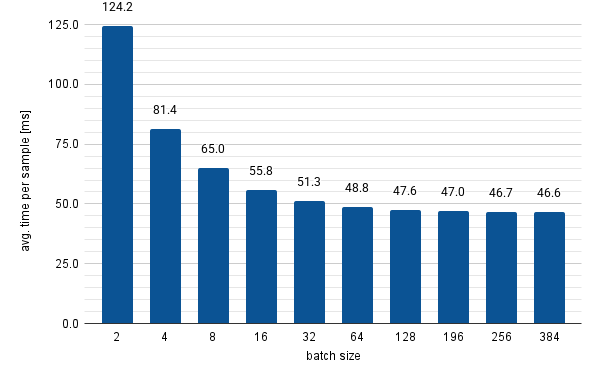
\includegraphics[width=0.75\textwidth]{Images/ivacic.latency_per_sample.png}
  \caption{Latency per sample for selected batch~sizes.}
  \label{fig:latency_per_sample}
\end{figure}
\vspace{-6pt}
\begin{table}[H]
  \centering
  \caption{Observed memory usage during inference on a single consumer-grade GPU. Values are means across 10 trials per batch; standard deviations were~negligible.}
  \label{tab:inference-memory}
  %\resizebox{0.65\textwidth}{!}{
  \begin{tabularx}{\textwidth}{l C}
    \toprule
    \textbf{Metric} & \textbf{Value} \\
    \midrule
    Model steady-state GPU memory & 1147.4~MB \\
    Peak GPU memory @ batch size $=2$ & 2645.0~MB \\
    Max allocated GPU memory @ batch size $=384$ & 7578.7~MB \\
    Peak host process memory & 2940.6~MB \\
    Knowledge memory (host) & 748.5~MB \\
    \bottomrule
  \end{tabularx}
  %}
\end{table}


%%%%%%%%%%%%%%%%%%%%%%%%%%%%%%%%%%%%%%%%%%
\section{Results}
\label{sec:results}

\subsection{Classification Performance~Analysis}
\label{sec:performance_analysis}
In this section, we present the results of our experiments. For~the primary analysis, we report micro- and macro-averaged F1-score, precision, and recall as label-based metrics, while subset accuracy is the example-based metric. 
We evaluate the SVM and Logistic Regression (LogReg) classifiers using the one-versus-all approach with TF-IDF representations (OVA-TFIDF) alongside a fine-tuned XLM-RoBERTa baseline (XLMR). 
In addition, we evaluate the original BGE-M3 model and the hard-negative fine-tuned BGE-M3 model (FT-BGE) across zero-shot, ML-KNN, and~simplified RAE-XMC methods.
All models are evaluated on the NewsMon\textsubscript{sl} and EURLEX57K datasets across all labels, followed by a detailed analysis of performance on frequent and rare labels. 
Finally, we conclude the result analysis by attributing the hard-negative fine-tuning and the modified RAE-XMC approach.



The first set of experimental results in Table~\ref{tab:result_newsmon_sl_all} shows that the FT-BGE retrieval model outperformed all other models on the NewsMon\textsubscript{sl} dataset across all metrics.
In terms of micro-averaged F1-score (micro-F1), macro-averaged precision, and~subset accuracy, the~simplified RAE-XMC method performed the best.
In contrast, the~zero-shot approach yielded the highest macro F1-score, primarily due to its superior recall.
Notably, even the non-fine-tuned BGE-M3 retrieval model outperformed the baseline with the RAE-XMC method across all metrics except for micro precision.
When examining the zero-shot performance improvement on the NewsMon\textsubscript{sl} dataset after fine-tuning the IR model, we observe an average gain of 16.7\% in micro-averaged metrics, 10.1\% in macro-averaged metrics, and~a 20.6\% increase in subset~accuracy.

\begin{table}[H]
    \small
    \caption{NewsMon\textsubscript{sl} (all labels): micro/macro F1, P, R, and~subset accuracy for SVM and logistic regression (OvA TF-IDF), XLM-RoBERTa baseline, BGE-M3, and~fine-tuned BGE-M3 under zero-shot, ML-KNN, and~RAE-XMC.}
%    \resizebox{0.65\textwidth}{!}{
%    \setlength{\tabcolsep}{3pt} % reduces column spacing
    \begin{tabularx}{\textwidth}{l l C c C c C c C}
        \toprule
        \multicolumn{1}{c}{\textbf{Model}} & 
        \multicolumn{1}{c}{\textbf{Method}} & 
        \multicolumn{1}{c}{\(\boldsymbol{\upmu}\)\textbf{F1}} &
        \multicolumn{1}{c}{\(\boldsymbol{\upmu}\)\textbf{P}} &
        \multicolumn{1}{c}{\(\boldsymbol{\upmu}\)\textbf{R}} &
        \multicolumn{1}{c}{\textbf{F1}} &
        \multicolumn{1}{c}{\textbf{P}} &
        \multicolumn{1}{c}{\textbf{R}} &
        \multicolumn{1}{c}{\textbf{Acc}} \\
        \midrule
        
%        Weak   & random       & 1.140  & 1.133  & 1.147  & 0.083  & 0.080  & 0.088  & 0.984   \\ 
%        Weak   & majority     & 5.782  & 5.735  & 5.830  & 0.010  & 0.005  & 0.093  & 0.000   \\ 
        SVM    & OVA-TFIDF    & 68.13 & 80.26 & 59.19 & 28.41 & \underline{34.00} & 26.26 & 44.88  \\ 
        LogReg & OVA-TFIDF    & 67.47 & 83.34 & 56.68 & 26.76 & 33.39 & 24.21 & 45.22 \\
        \midrule
        XLMR   & baseline     & 53.50 & 85.21 & 39.17 & 4.70  & 6.81  & 3.99  & 38.02  \\
        \midrule
        BGE-M3 & zshot        & 59.04 & 55.84 & 62.62 & 28.28 & 28.12 & \underline{31.18} & 42.58  \\
        BGE-M3 & ML-KNN       & 42.94 & 77.94 & 29.63 & 5.92  & 9.77  & 4.78  & 29.63  \\
        BGE-M3 & RAE-XMC      & 65.58 & 76.11 & 57.61 & 28.18 & 32.61 & 26.88 & 44.49  \\
        \midrule
        FT-BGE & zshot        & \underline{68.93} & 67.20 & \textbf{70.75} & \textbf{31.21} & 31.71 & \textbf{33.47} & \underline{51.38}  \\
        FT-BGE & ML-KNN       & 62.18 & \textbf{86.48} & 48.54 & 9.30  & 13.47 & 7.89  & 46.67  \\
        FT-BGE & RAE-XMC      & \textbf{73.67} & \underline{86.07} & \underline{64.39} & \underline{29.24} & \textbf{34.64} & 27.27 & \textbf{56.12}  \\
        \bottomrule
        %\multicolumn{9}{c}{best results are bolded, second best are underlined} \\
    \end{tabularx}
        \footnotesize {\textbf{Note:} Best results are shown in \textbf{bold}, and~second-best results are \underline{underlined}.}
   % }
    \label{tab:result_newsmon_sl_all}
\end{table}


An examination of the EURLEX57K dataset experiment results in Table~\ref{tab:result_eurlex_all} reveals that the micro-averaged F1-score and precision are significantly lower for the RAE-XMC method than the baseline. 
Conversely, the~fine-tuned BGE-M3 model, combined with the modified RAE-XMC method, achieved the highest macro-averaged F1-score and subset accuracy.

\begin{table}[H]
    \small
    \caption{EURLEX57K (all labels): micro/macro F1, P, R, and~subset accuracy for SVM and logistic regression (OvA TF-IDF), XLM-RoBERTa baseline, BGE-M3, and~fine-tuned BGE-M3 under zero-shot, ML-KNN, and~RAE-XMC.}
%    \resizebox{0.65\textwidth}{!}{
%    \setlength{\tabcolsep}{3pt} % reduces column spacing
    \begin{tabularx}{\textwidth}{l l C c C c C c C}
        \toprule
        \multicolumn{1}{c}{\textbf{Model}} & 
        \multicolumn{1}{c}{\textbf{Method}} & 
        \multicolumn{1}{c}{\(\boldsymbol{\upmu}\)\textbf{F1}} &
        \multicolumn{1}{c}{\(\boldsymbol{\upmu}\)\textbf{P}} &
        \multicolumn{1}{c}{\(\boldsymbol{\upmu}\)\textbf{R}} &
        \multicolumn{1}{c}{\textbf{F1}} &
        \multicolumn{1}{c}{\textbf{P}} &
        \multicolumn{1}{c}{\textbf{R}} &
        \multicolumn{1}{c}{\textbf{Acc}} \\
       
        \midrule
%        Weak   & random       & 1.728   & 1.734   & 1.721   & 0.122   & 0.125   & 0.122   & 0.053   \\
%        Weak   & majority     & 6.448   & 6.516   & 6.381   & 0.014   & 0.008   & 0.117   & 0.000   \\
        SVM    & OVA-TFIDF    & \underline{73.21}  & \underline{82.92}  & 65.54  & 25.65  & \textbf{30.98}  & 23.58  & \underline{25.58}  \\
        LogReg & OVA-TFIDF    & 71.61  & 82.07 & 63.51 & 23.84 & 29.38 & 21.63 & 22.34 \\
        \midrule
        XLMR   & baseline     & \textbf{75.98}  & \textbf{93.18}  & 64.14  & 13.95  & 18.83  & 12.19  & 24.25  \\
        \midrule
        BGE-M3 & zshot        & 66.52  & 66.67  & 66.37  & 25.65  & 26.74  & 26.76  & 23.12  \\
        BGE-M3 & ML-KNN       & 57.68  & 81.49  & 44.63  & 9.63   & 14.50  & 8.03   & 11.77  \\
        BGE-M3 & RAE-XMC      & 69.72  & 74.63  & 65.41  & 25.73  & 28.69  & 25.11  & 23.47  \\
        \midrule
        FT-BGE & zshot        & 68.37  & 68.40  & \textbf{68.33}  & \underline{26.81}  & 27.95  & \textbf{28.00}  & 25.58  \\
        FT-BGE & ML-KNN       & 59.96  & 82.54  & 47.08  & 10.55  & 15.51  & 8.92   & 12.84  \\
        FT-BGE & RAE-XMC      & 69.99  & 72.35  & \underline{67.77}  & \textbf{27.12}  & \underline{29.42}  & \underline{27.25}  & \textbf{25.91}  \\
        \midrule
    \end{tabularx}
    %}
       \footnotesize {\textbf{Note:} Best results are shown in \textbf{bold}, and~second-best results are \underline{underlined}.}
    \label{tab:result_eurlex_all}
\end{table}
However, the~zero-shot method demonstrates higher recall than RAE-XMC, consistent with the findings from the previous set of experiments on NewsMon\textsubscript{sl}. 
These findings suggest that further enhancements are needed to improve the recall of our approach compared to the zero-shot method. 
Moreover, improvements in micro-averaged F1-score and precision are also required to surpass the baseline performance for the EURLEX57K dataset.
We hypothesise that this outcome can be attributed to a combination of the following~factors:
\begin{itemize}
    \item The relatively worse performance of multilingual models on English-language tasks, as~evidenced by differences in zero-shot performance (see Tables~\ref{tab:zero_ir_newsmonsl} and \ref{tab:zero_ir_eurlex}) and MTEB benchmark rankings (Table \ref{tab:model_specs});
    \item The higher degree of label diversity present in the EURLEX57K dataset, which makes correct predictions harder;
    \item The suboptimal performance of our method on the frequent labels within this dataset \mbox{(see Table~\ref{tab:result_newsmon_sl_frequent} in comparison to Table~\ref{tab:result_eurlex_frequent}).}
\end{itemize}

Notably, the~SVM classifier outperforms the baseline in terms of subset accuracy and achieves the highest macro-averaged precision among all evaluated~models.

Similarly, we observe a zero-shot performance improvement on the EURLEX57K dataset after fine-tuning the IR model, with~an average gain of 2.8\% in micro-averaged metrics, 4.5\% in macro-averaged metrics, and~a 10.6\% increase in subset~accuracy.


For frequent (head) labels in NewsMon\textsubscript{sl} that appear 500 times or more (see Table~\ref{tab:result_newsmon_sl_frequent}), the~FT-BGE model combined with the modified RAE-XMC approach outperformed all other models in terms of F1-score, precision, and~subset accuracy. The~exceptions were recall, where the zero-shot method performed best, consistent with the results observed in our initial experiments across all labels.
If we observe only the non-modified BGE-M3 model, we can see that its performance does not surpass the baseline in this third set of~experiments.

\begin{table}[H]
    \small
    \caption{NewsMon\textsubscript{sl} (frequent labels): micro/macro F1, P, R, and~subset accuracy for SVM and logistic regression (OvA TF-IDF), XLM-RoBERTa baseline, BGE-M3, and~fine-tuned BGE-M3 under zero-shot, ML-KNN, and~RAE-XMC.}
%    \resizebox{0.65\textwidth}{!}{
%    \setlength{\tabcolsep}{3pt} % reduces column spacing
    \begin{tabularx}{\textwidth}{l l C c C c C c C}
        \toprule
        \multicolumn{1}{c}{\textbf{Model}} & 
        \multicolumn{1}{c}{\textbf{Method}} & 
        \multicolumn{1}{c}{\(\boldsymbol{\upmu}\)\textbf{F1}} &
        \multicolumn{1}{c}{\(\boldsymbol{\upmu}\)\textbf{P}} &
        \multicolumn{1}{c}{\(\boldsymbol{\upmu}\)\textbf{R}} &
        \multicolumn{1}{c}{\textbf{F1}} &
        \multicolumn{1}{c}{\textbf{P}} &
        \multicolumn{1}{c}{\textbf{R}} &
        \multicolumn{1}{c}{\textbf{Acc}} \\
        \midrule
       
%        Weak   & random       & 4.246   & 4.243   & 4.249   & 3.212   & 3.206   & 3.233   & 3.043   \\
%        Weak   & majority     & 10.211  & 9.201   & 11.470  & 0.661   & 0.361   & 3.922   & 0.000   \\
        SVM    & OVA-TFIDF    & 81.40 & 88.43 & 75.40 & 77.41 & 86.29 & 70.87 & 67.35 \\
        LogReg & OVA-TFIDF    & 81.55 & 90.54 & 74.18 & 77.23 & 88.48 & 69.34 & 67.79 \\
        \midrule
        XLMR   & baseline     & 82.65  & 90.24  & 76.29  & 77.24  & 86.99  & 70.98  & 70.26  \\
        \midrule
        BGE-M3 & zshot        & 76.41  & 78.41  & 74.51  & 72.63  & 75.67  & 70.63  & 65.77  \\
        BGE-M3 & ML-KNN       & 66.15  & 85.25  & 54.05  & 56.36  & 81.71  & 45.97  & 50.18  \\
        BGE-M3 & RAE-XMC      & 78.96  & 87.44  & 71.97  & 74.20  & 85.08  & 67.13  & 66.24  \\
        \midrule
        FT-BGE & zshot        & \underline{86.71}  & 87.39  & \textbf{86.05}  & \underline{83.42}  & 84.89  & \textbf{82.60}  & \underline{78.09}  \\
        FT-BGE & ML-KNN       & 86.22  & \underline{91.56}  & 81.47  & 81.62  & \underline{89.18}  & 76.55  & 76.36  \\
        FT-BGE & RAE-XMC      & \textbf{88.31}  & \textbf{93.59}  & \underline{83.59}  & \textbf{84.51}  & \textbf{91.35}  & \underline{79.40}  & \textbf{79.64}  \\
        \bottomrule
    \end{tabularx}
        \footnotesize {\textbf{Note:} Best results are shown in \textbf{bold}, and~second-best results are \underline{underlined}.}
   % }
    \label{tab:result_newsmon_sl_frequent}
\end{table}
\vspace{-6pt}
\begin{table}[H]
    \small
    \caption{EURLEX57K (frequent labels): micro/macro F1, P, R, and~subset accuracy for SVM and logistic regression (OvA TF-IDF), XLM-RoBERTa baseline, BGE-M3, and~fine-tuned BGE-M3 under zero-shot, ML-KNN, and~RAE-XMC.}
%    \resizebox{0.65\textwidth}{!}{
%    \setlength{\tabcolsep}{3pt} % reduces column spacing
    \begin{tabularx}{\textwidth}{l l C c C c C c C}
        \toprule
        \multicolumn{1}{c}{\textbf{Model}} & 
        \multicolumn{1}{c}{\textbf{Method}} & 
        \multicolumn{1}{c}{\(\boldsymbol{\upmu}\)\textbf{F1}} &
        \multicolumn{1}{c}{\(\boldsymbol{\upmu}\)\textbf{P}} &
        \multicolumn{1}{c}{\(\boldsymbol{\upmu}\)\textbf{R}} &
        \multicolumn{1}{c}{\textbf{F1}} &
        \multicolumn{1}{c}{\textbf{P}} &
        \multicolumn{1}{c}{\textbf{R}} &
        \multicolumn{1}{c}{\textbf{Acc}} \\
        \midrule
    
%        Weak   & random       & 3.591   & 3.594   & 3.588   & 2.378   & 2.400   & 2.376   & 0.141   \\
%        Weak   & majority     & 8.385   & 8.180   & 8.599   & 0.374   & 0.203   & 2.479   & 0.000   \\
        SVM    & OVA-TFIDF    & \underline{82.26} & \underline{87.24} & 77.82 & \underline{79.74} & \underline{85.40} & 75.62 & \underline{46.56} \\
        LogReg & OVA-TFIDF    & 80.63 & 85.81 & 76.05 & 77.88 & 83.99 & 73.33 & 43.10 \\
        \midrule
        XLMR   & baseline     & \textbf{90.18}  & \textbf{94.15}  & \textbf{86.54}  & \textbf{87.56}  & \textbf{93.39}  & \textbf{83.95}  & \textbf{62.79}  \\
        \midrule
        BGE-M3 & zshot        & 77.45  & 78.00  & 76.91  & 74.51  & 75.34  & 73.97  & 40.68  \\
        BGE-M3 & ML-KNN       & 72.46  & 84.55  & 63.39  & 65.64  & 80.44  & 58.57  & 29.04  \\
        BGE-M3 & RAE-XMC      & 80.02  & 83.06  & 77.20  & 76.87  & 80.46  & 74.11  & 43.30  \\
        \midrule
        FT-BGE & zshot        & 79.02  & 79.53  & \underline{78.52}  & 76.35  & 76.99  & \underline{75.93}  & 43.59  \\
        FT-BGE & ML-KNN       & 74.29  & 85.31  & 65.79  & 68.49  & 81.49  & 61.66  & 31.65  \\
        FT-BGE & RAE-XMC      & 80.05  & 81.71  & 78.46  & 77.40  & 79.32  & 75.85  & 44.86  \\
        \bottomrule
    \end{tabularx}
        \footnotesize {\textbf{Note:} Best results are shown in \textbf{bold}, and~second-best results are \underline{underlined}.}
  %  }
    \label{tab:result_eurlex_frequent}
\end{table}
In contrast, the~fourth set of experiments on EURLEX57K indicates that our approach fell significantly short of surpassing the baseline. 
This result suggests that the XLMR model exhibits substantially stronger classification performance for the English language when presented with enough training samples and a smaller label space (see Table~\ref{tab:result_eurlex_frequent}). This suggests that an optimal approach could involve a gated ensemble of classifiers based on label frequency. However, the~dynamic nature of the label space, coupled with the inconsistent results observed on the frequent labels of the NewsMon\textsubscript{sl} dataset, presents significant challenges to this approach. In~experiments involving frequent labels, we observe that the macro-averaged F1 score can be relatively high even when the subset accuracy remains low. This discrepancy arises from the fundamental difference between the two metrics: macro F1 evaluates performance at the class level, while subset accuracy operates at the instance level. As~a result, a~model may perform well when assessed per label but struggle to predict all labels correctly for a given instance. Moreover, subset accuracy is an ``all-or-nothing'' metric, highlighting that the model often predicts some, but~not all, of~the correct labels. Compared to the first two experiments, where subset accuracy exceeded macro F1, the~influence of rare labels in this setting leads to the opposite effect on these~metrics.

Finally, when analysing the performance on rare (tail) labels, it is evident that ML-KNN and the baseline approach performed~poorly.


In both sets of experiments on the EURLEX57K and NewsMon\textsubscript{sl} datasets, the~baseline and ML-KNN models were unable to classify rare labels effectively, as~shown in \mbox{Tables~\ref{tab:result_newsmon_sl_rare} and ~\ref{tab:result_eurlex_rare}.}
This implies that a minimal amount of training data is insufficient for these approaches to be effective.
Interestingly, in~experiments on rare labels within the EURLEX57K and NewsMon\textsubscript{sl} datasets, both zero-shot methods outperformed the simplified RAE-XMC approach in terms of~accuracy.

\begin{table}[H]
    \small
    \caption{NewsMon\textsubscript{sl} (rare labels): micro/macro F1, P, R, and~subset accuracy for SVM and logistic regression (OvA TF-IDF), XLM-RoBERTa baseline, BGE-M3, and~fine-tuned BGE-M3 under zero-shot, ML-KNN, and~RAE-XMC.}
%    \resizebox{0.65\textwidth}{!}{
%    \setlength{\tabcolsep}{3pt} % reduces column spacing
    \begin{tabularx}{\textwidth}{l l C c C c C c C}
        \toprule
        \multicolumn{1}{c}{\textbf{Model}} & 
        \multicolumn{1}{c}{\textbf{Method}} & 
        \multicolumn{1}{c}{\(\boldsymbol{\upmu}\)\textbf{F1}} &
        \multicolumn{1}{c}{\(\boldsymbol{\upmu}\)\textbf{P}} &
        \multicolumn{1}{c}{\(\boldsymbol{\upmu}\)\textbf{R}} &
        \multicolumn{1}{c}{\textbf{F1}} &
        \multicolumn{1}{c}{\textbf{P}} &
        \multicolumn{1}{c}{\textbf{R}} &
        \multicolumn{1}{c}{\textbf{Acc}} \\
        \midrule
      
%        Weak   & random       & 0.000   & 0.000   & 0.000   & 0.000   & 0.000   & 0.000   & 0.000   \\
%        Weak   & majority     & 0.000   & 0.000   & 0.000   & 0.000   & 0.000   & 0.000   & 0.000   \\
        SVM    & OVA-TFIDF    & 49.12  & 90.15  & 33.76  & 11.81  & 12.65  & 11.42  & 27.51  \\
        LogReg & OVA-TFIDF    & 45.06  & \underline{92.51}  & 29.79  & 10.55  & 11.32  & 10.18  & 24.24  \\
        \midrule
        XLMR   & baseline     & 0.00   & 0.00   & 0.00   & 0.00   & 0.00   & 0.00   & 0.00   \\
        \midrule
        BGE-M3 & zshot        & \underline{52.59}  & 71.70  & \underline{41.53}  & \underline{14.72}  & \underline{15.52}  & \underline{14.45}  & \underline{33.12}  \\
        BGE-M3 & ML-KNN       & 0.00   & 0.00   & 0.00   & 0.06   & 0.06   & 0.06   & 0.00   \\
        BGE-M3 & RAE-XMC      & 50.20  & 90.58  & 34.72  & 12.53  & 13.45  & 12.09  & 27.96  \\
        \midrule
        FT-BGE & zshot        & \textbf{55.00}  & 73.66  & \textbf{43.89}  & \textbf{15.06}  & \textbf{15.64}  & \textbf{15.15}  & \textbf{34.84}  \\
        FT-BGE & ML-KNN       & 0.00   & 0.00   & 0.00   & 0.06   & 0.06   & 0.06   & 0.00   \\
        FT-BGE & RAE-XMC      & 48.30  & \textbf{92.89}  & 32.64  & 11.93  & 12.88  & 11.46  & 26.02  \\
        \bottomrule
    \end{tabularx}
       \footnotesize {\textbf{Note:} Best results are shown in \textbf{bold}, and~second-best results are \underline{underlined}.}
   % }
    \label{tab:result_newsmon_sl_rare}
\end{table}
\vspace{-6pt}

\begin{table}[H]
    \small
    \caption{EURLEX57K (rare labels): micro/macro F1, P, R, and~subset accuracy for SVM and logistic regression (OvA TF-IDF), XLM-RoBERTa baseline, BGE-M3, and~fine-tuned BGE-M3 under zero-shot, ML-KNN, and~RAE-XMC.}
%    \resizebox{0.65\textwidth}{!}{
%    \setlength{\tabcolsep}{3pt} % reduces column spacing
    \begin{tabularx}{\textwidth}{l l l l C c C c C c C}
        \toprule
        \multicolumn{1}{c}{\textbf{Model}} & 
        \multicolumn{1}{c}{\textbf{Method}} & 
        \multicolumn{1}{c}{\(\boldsymbol{\upmu}\)\textbf{F1}} &
        \multicolumn{1}{c}{\(\boldsymbol{\upmu}\)\textbf{P}} &
        \multicolumn{1}{c}{\(\boldsymbol{\upmu}\)\textbf{R}} &
        \multicolumn{1}{c}{\textbf{F1}} &
        \multicolumn{1}{c}{\textbf{P}} &
        \multicolumn{1}{c}{\textbf{R}} &
        \multicolumn{1}{c}{\textbf{Acc}} \\
        \midrule
      
%        Weak   & random       & 0.000   & 0.000   & 0.000   & 0.000   & 0.000   & 0.000   & 0.000   \\
%        Weak   & majority     & 0.000   & 0.000   & 0.000   & 0.000   & 0.000   & 0.000   & 0.000   \\
        SVM    & OVA-TFIDF    & 26.57  & \underline{72.19}  & 16.28  & 4.95  & 5.43  & 4.78  & 14.07 \\
        LogReg & OVA-TFIDF    & 30.19  & \textbf{78.28}  & 18.70  & 5.57  & 6.15  & 5.33  & 18.76 \\
        \midrule
        XLMR   & baseline     & 0.52   & 0.00   & 0.26   & 0.05   & 0.08   & 0.04   & 0.28   \\
        \midrule
        BGE-M3 & zshot        & 34.14  & 47.32  & \underline{26.70}  & \underline{8.10}   & 8.81   & \underline{8.00}   & 20.60  \\
        BGE-M3 & ML-KNN       & 0.00   & 0.00   & 0.00   & 0.00   & 0.00   & 0.00   & 0.00   \\
        BGE-M3 & RAE-XMC      & 33.38  & 57.87  & 23.46  & 7.27   & 7.94   & 7.07   & 18.04  \\
        \midrule
        FT-BGE & zshot        & \underline{36.21}  & 50.19  & \textbf{28.32}  & \textbf{8.40}   & \textbf{9.19}   & \textbf{8.24}   & \textbf{22.59}  \\
        FT-BGE & ML-KNN       & 0.00   & 0.00   & 0.00   & 0.00   & 0.00   & 0.00   & 0.00   \\
        FT-BGE & RAE-XMC      & \textbf{36.48}  & 57.58  & 26.70  & 7.97   & \underline{8.81}                                             & 7.78   & \underline{21.88}  \\
        \bottomrule
    \end{tabularx}
        \footnotesize {\textbf{Note:} Best results are shown in \textbf{bold}, and~second-best results are \underline{underlined}.}
    %}
    \label{tab:result_eurlex_rare}
\end{table}

\subsection{Factor Attribution~Analysis}
\label{sec:factor_attribution_analysis} 



Most gains come from hard-negative fine-tuning; RAE-XMC adds precision but slightly hurts tail recall (See Table~\ref{tab:factor_attribution} for deltas by factor.).
On the NewsMon\textsubscript{sl} dataset, most of the gains stem from hard-negative (HN) fine-tuning of the retriever, which yields $+9.89$\,pp for micro-F1 and $+8.80$\,pp for subset accuracy, relative to the zero-shot 1‑Nearest Neighbour (1-NN) retriever without fine-tuning.
The RAE-XMC retrieval/predictor contributes a smaller, precision-oriented boost ($+6.54$\,pp for micro-F1 and $+1.91$\,pp for accuracy over 1-NN with the same encoder), but~slightly reduces tail performance, consistent with softmax-weighted neighbour aggregation favouring head labels (i.e., neighbour weighting skews toward frequent labels; \cref{tab:result_newsmon_sl_all,tab:result_eurlex_all,tab:result_newsmon_sl_frequent,tab:result_eurlex_frequent,tab:result_newsmon_sl_rare,tab:result_eurlex_rare}). 
We expect hard-negative (HN) fine-tuning to increase classification recall through improved retrieval precision, since it makes the retriever more discriminative (retrieved neighbours are more likely to share true labels with the query). On~the other hand, we expect the RAE-XMC retrieval/predictor mechanism, a~softmax-weighted averaging over multiple neighbours, to~increase classification precision.
For the NewsMon\textsubscript{sl}, the~interaction between RAE-XMC and HN is mildly negative for micro-F1 (all: $-1.80$\,pp, frequent: $-0.95$\,pp, rare: $-4.31$\,pp) and slightly positive for subset accuracy on the all and frequent splits (all: $+2.83$\,pp, frequent: $+1.08$\,pp) but negative on the rare split ($-3.66$\,pp), indicating overlapping effects on recall and complementary effects on precision, consistent with the observation that adding RAE-XMC after HN does not increase~recall.

\begin{table}[H]
    %\centering
\small
    \caption{Factor attribution (absolute \%-point deltas) for the effects of hard-negative fine-tuning (HN), RAE-XMC retrieval, and~their interaction across datasets and label~subsets.}
%    \resizebox{0.95\textwidth}{!}{
%    \setlength{\tabcolsep}{3pt}
    
\begin{adjustwidth}{-\extralength}{0cm}
%\centering %% If there is a figure in wide page, please release command \centering
\begin{tabularx}{\fulllength}{l c c c c c c c c}
        \toprule
        \multicolumn{1}{c}{\textbf{Dataset/Split}} &
        \multicolumn{1}{c}{\(\Delta\)\(\boldsymbol{\upmu}\)\textbf{F1 HN}} &
        \multicolumn{1}{c}{\(\Delta\)\(\boldsymbol{\upmu}\)\textbf{F1 RAE}} &
        \multicolumn{1}{c}{\(\Delta\)\(\boldsymbol{\upmu}\)\textbf{F1 Int.}} &
        \multicolumn{1}{c}{\(\Delta\)\(\boldsymbol{\upmu}\)\textbf{F1 Total}} &
        \multicolumn{1}{c}{\(\Delta\)\textbf{Acc HN}} &
        \multicolumn{1}{c}{\(\Delta\)\textbf{Acc RAE}} &
        \multicolumn{1}{c}{\(\Delta\)\textbf{Acc Int.}} &
        \multicolumn{1}{c}{\(\Delta\)\textbf{Acc Total}} \\
        \midrule
       
        NewsMon\textsubscript{sl} (All)     & +9.89  & +6.54  & $-$1.80 & +14.63 & +8.80  & +1.91 & +2.83 & +13.54 \\
        NewsMon\textsubscript{sl} (Frequent) & +10.30 & +2.55  & $-$0.95 & +11.90 & +12.32 & +0.47 & +1.08 & +13.87 \\
        NewsMon\textsubscript{sl} (Rare)     & +2.41  & $-$2.39  & $-$4.31 & $-$4.29  & +1.72  & $-$5.16 & $-$3.66 & $-$7.10 \\
        EURLEX57K (All)                     & +1.85  & +3.20  & $-$1.58 & +3.47  & +2.46  & +0.35 & $-$0.02 & +2.79 \\
        EURLEX57K (Frequent)                & +1.57  & +2.58  & $-$1.55 & +2.60  & +2.91  & +2.63 & $-$1.35 & +4.18 \\
        EURLEX57K (Rare)                    & +2.07  & $-$0.75  & +1.03 & +2.34  & +1.99  & $-$2.56 & +1.85 & +1.28 \\
        \bottomrule
    \end{tabularx}
\end{adjustwidth}
   %}
               \footnotesize {\textbf{Note:} “HN” = hard-negative fine-tuning effect (FT-BGE zero-shot – BGE-M3 zero-shot); “RAE” = RAE-XMC retrieval/predictor effect (BGE-M3 RAE – BGE-M3 zero-shot); “Int.” = interaction term explaining residual; \mbox{“Total” = overall} delta from BGE-M3 zero-shot → FT-BGE RAE-XMC. Values derived from \cref{tab:result_newsmon_sl_all,tab:result_eurlex_all,tab:result_newsmon_sl_frequent,tab:result_eurlex_frequent,tab:result_newsmon_sl_rare,tab:result_eurlex_rare}.
        }
    \label{tab:factor_attribution}
\end{table}

On EURLEX57K, both components contribute small, partially overlapping improvements (from \(+1.85\)\,pp to \(+3.20\)\,pp for micro-F1 and from \(+0.35\)\,pp to \(+2.46\)\,pp for accuracy), and~their interaction term is near-zero for accuracy, indicating largely additive~effects. 

Overall, on~NewsMon\textsubscript{sl}, hard-negative fine-tuning is the primary driver of improvement. 
At the same time, the~RAE-XMC retrieval/predictor yields smaller but consistent gains on the \emph{all} and \emph{frequent} splits across both datasets. 
For the \emph{rare} split, the~modified RAE-XMC generally reduces performance, so it should be applied with caution on tails.
We hypothesise that the larger gains on NewsMon\textsubscript{sl} versus EURLEX57K could also arise from the keyword-driven labelling pipeline in NewsMon\textsubscript{sl} (Section~\ref{sec:data_description}, Table~\ref{tab:kwes}), which introduces lexical “anchors” that retrieval can exploit. 
%Additionally, NewsMon\textsubscript{sl} label selection and labelling quality are inconsistent, whereas EURLEX57K texts are labelled with a broad EuroVoc concept hierarchical label space.
%We further identify several dataset-specific factors that may inflate apparent gains, notably the longer input sequences in NewsMon\textsubscript{sl} (approximately half of all samples exceed 512 tokens, see Figure~\ref{fig:tokens_hist} in Section~\ref{sec:related_work}) and the keyword-driven labelling pipeline (Section~\ref{sec:data_description}, Table~\ref{tab:kwes}), both of which favour retrieval-based methods over the truncated XLM-R baseline.
%%%%%%%%%%%%%%%%%%%%%%%%%%%%%%%%%%%%%%%%%%

\section{Conclusions: Summary of Advances and Lessons~Learned}
\label{sec:conclusions}

We demonstrate that information retrieval (IR) models outperform end-to-end fine-tuned approaches in settings with a large number of labels when dealing with less-represented languages. Furthermore, our IR-based method demonstrates a degree of effectiveness even without fine-tuning, making it well-suited for continuously evolving systems with dynamic label spaces, particularly when scalability to an arbitrary label space is a critical~requirement.

The results indicate that while our approach surpasses the XLMR baseline on the NewsMon\textsubscript{sl} dataset, the~overall findings for both datasets remain inconclusive. 
Specifically, our approach outperforms the XLMR baseline across all reported metrics on the NewsMon\textsubscript{sl} dataset, where HN fine-tuning is the largest contributor. 
However, on~EURLEX57K, the~micro-averaged F1-score and precision remain lower than those of the baseline. 
In particular, on~the EURLEX57K dataset, where labels are more consistent and data are predominantly in English, the~method leaves room for improvement, as our method surpassed the baselines only on macro-averaged scores and subset~accuracy.

These findings suggest that pre-trained, end-to-end fine-tuned models may be more effective for tasks in the predominant language used during model pre-training, particularly when the number of model parameters is limited due to resource constraints~\citep{chang2023multilingualitycurselanguagemodeling}.
In contrast, multilingual IR models tend to underperform in comparison. 
Both observations underscore the importance of fairness in the design of multilingual models.
Less-represented languages are often under-resourced and underrepresented in large-scale pre-training corpora, resulting in lower quality representations and limited task performance~\citep{gupta2025multilingualperformancebiaseslarge}.
Nevertheless, retrieval-based models excel with rare labels, even when no fine-tuning is applied.
As a result, the~findings for research question RQ1 remain inconclusive across both datasets, underscoring the need for further investigation and refinement of our approach in high-resource, monolingual~settings.

On the other hand, zero-shot and unchanged IR model experiments demonstrate that pre-trained multilingual retrieval models can be used effectively (RQ3), as~also suggested by~\citep{wang2025retrievalaugmentedencodersextrememultilabel}, provided that the predictor component is further improved or a true dual-encoder architecture is employed~\citep{gupta2024dexml}.

This also addresses the research question RQ2, indicating that while the method's effectiveness without label descriptions is limited, it presents new research opportunities. 
In particular, incorporating a trainable $\lambda$ vector or matrix model that assigns importance to the labels of each training sample could enhance~performance.

Furthermore, we demonstrate that incorporating contrastive learning with hard negative sampling further improves the IR model within our classification setting, addressing research question RQ4.
Given that the simplified RAE-XMC method outperformed the XLMR baseline without requiring fine-tuning on the NewsMon\textsubscript{sl} dataset, our results demonstrate the potential for developing a method suitable for rapid label updates. Moreover, the~approach relies on a model with fewer than one billion parameters, making it well-suited for low-resource~environments. 

%Notably, the method is language-agnostic and thus applicable to underrepresented or low-resource languages such as Slovene and Serbian.
%However, we acknowledge that pre-trained language models inherently carry the perspectives of dominant linguistic and cultural groups present in pre-training corpora~\citep{nie-etal-2024-multilingual}. 
%Nevertheless, in our setting, where the primary use case involves similarity search within a given language's knowledge memory, cultural or social biases are primarily contained within that language. 
%As a result, given the multilingual encoder model selection and retrieval-based approach, it is less likely for bias to amplify or transfer across languages. 
%Unlike tasks such as sentiment analysis or hate speech detection, which are sensitive to sociocultural nuance, our method tends to preserve or even attenuate existing biases within the original language boundaries~\citep{levy-etal-2023-comparing}.

Notably, the~proposed method is language-agnostic and thus applicable to less-represented or low-resource languages, such as Slovene and Serbian, as~the underlying retrieval models were not specifically fine-tuned on these languages. 
Although we did not conduct cross-lingual experiments, we believe the approach can be effectively extended to cross-lingual settings, provided the retriever exhibits strong cross-lingual alignment and is fine-tuned with hard negatives drawn from datasets across all target languages; such transfer is likely to be especially effective for languages within the same family (see Appendix~\ref{subsec:sr_mk_preliminary} of preliminary research).

Additionally, our information retrieval approach enhances scalability further through the use of knowledge memory embeddings per language and model. 
This compact embedding footprint enables the system to efficiently support numerous languages in parallel or even with a single model. 
Importantly, these knowledge memory embeddings can be offloaded to external retrieval systems when needed, allowing for flexible deployment on various hardware configurations and seamless integration with scalable, distributed retrieval~infrastructures.

%Furthermore, although we did not conduct experiments in a cross-lingual setting, we believe the proposed method could be effectively extended to such scenarios, assuming the retrieval model has strong cross-lingual capabilities and is fine-tuned with hard negatives drawn from datasets across all target languages, especially when languages from the same family are considered. 
%However, this assumption may not hold for highly divergent low-resource languages like Sanskrit or Hindi. 
%These languages can have very different grammatical structures, word orders, or morphological systems compared to high-resource languages (like English, French, or German), which are usually the primary focus of NLP models and datasets~\citep{pakray2025lowresourcenlp, sahupal2025}.

\section{Future~Work}
\label{sec:future}

Future work will focus on several key areas of improvement to enhance the classification model and consequently improve the reliability of result interpretation.
First, we plan to extend the pre-training of our models to include the Serbian, Bosnian, Croatian, and~Macedonian languages, allowing us to assess the effectiveness of our methods in a truly multilingual context (see Appendix~\ref{subsec:sr_mk_preliminary} for preliminary research).
%Next, we aim to broaden our experiments by incorporating additional multi-label text classification datasets with similar label distribution characteristics.
Additionally, we will explore the impact of fine-tuning the IR model on generalisation and its applicability to unseen labels.
Finally, we intend to leverage the provided simplified Keyword-Boolean expressions to identify label-relevant text passages and experiment with smaller text samples, which could help improve precision.
This approach may also facilitate the generation of synthetic label descriptions, which could be used in contrastive learning to enhance precision~further. 

%%%%%%%%%%%%%%%%%%%%%%%%%%%%%%%%%%%%%%%%%%
\vspace{6pt} 

%%%%%%%%%%%%%%%%%%%%%%%%%%%%%%%%%%%%%%%%%%
%% optional
%\supplementary{The following supporting information can be downloaded at:  \linksupplementary{s1}, Figure S1: title; Table S1: title; Video S1: title.}

% Only for journal Methods and Protocols:
% If you wish to submit a video article, please do so with any other supplementary material.
% \supplementary{The following supporting information can be downloaded at: \linksupplementary{s1}, Figure S1: title; Table S1: title; Video S1: title. A supporting video article is available at doi: link.}

% Only used for preprints:
% \supplementary{The following supporting information can be downloaded at the website of this paper posted on \href{https://www.preprints.org/}{Preprints.org}.}

% Only for journal Hardware:
% If you wish to submit a video article, please do so with any other supplementary material.
% \supplementary{The following supporting information can be downloaded at: \linksupplementary{s1}, Figure S1: title; Table S1: title; Video S1: title.\vspace{6pt}\\
%\begin{tabularx}{\textwidth}{lll}
%\toprule
%\textbf{Name} & \textbf{Type} & \textbf{Description} \\
%\midrule
%S1 & Python script (.py) & Script of python source code used in XX \\
%S2 & Text (.txt) & Script of modelling code used to make Figure X \\
%S3 & Text (.txt) & Raw data from experiment X \\
%S4 & Video (.mp4) & Video demonstrating the hardware in use \\
%\dots & \dots & \dots \\
%\bottomrule
%\end{tabularx}
%}

%%%%%%%%%%%%%%%%%%%%%%%%%%%%%%%%%%%%%%%%%%
\authorcontributions{Conceptualization, N.I.; methodology, N.I., B.Š. and~B.K.; software, N.I.; validation, B.Š., B.K. and~M.P.; formal analysis, B.Š., B.K. and~M.P.; investigation, N.I., B.Š. and~B.K.; resources, N.I.; data curation, N.I.; writing—original draft preparation, N.I. and N.L.; writing—review and editing, S.P., N.L. and~M.P.; visualization, B.Š.; supervision, S.P., N.L. and~M.P.; project administration, S.P. and N.L.; funding acquisition, S.P. and N.L. All authors have read and agreed to the published version of the~manuscript.}

\funding{This work was funded by the Slovenian Research and Innovation Agency (ARIS) through grants GC-0002 (Large Language Models for Digital Humanities) and the core research programme P2-0103 (Knowledge Technologies). The~work of B.K. was supported by the Young Researcher Grant PR-12394. This work was partially funded by the ARIS project L2-50070.
}

%\institutionalreview{In this section, you should add the Institutional Review Board Statement and approval number, if relevant to your study. You might choose to exclude this statement if the study did not require ethical approval. Please note that the Editorial Office might ask you for further information. Please add “The study was conducted in accordance with the Declaration of Helsinki, and approved by the Institutional Review Board (or Ethics Committee) of NAME OF INSTITUTE (protocol code XXX and date of approval)” for studies involving humans. OR “The animal study protocol was approved by the Institutional Review Board (or Ethics Committee) of NAME OF INSTITUTE (protocol code XXX and date of approval)” for studies involving animals. OR “Ethical review and approval were waived for this study due to REASON (please provide a detailed justification).” OR “Not applicable” for studies not involving humans or animals.}

%\informedconsent{Any research article describing a study involving humans should contain this statement. Please add ``Informed consent was obtained from all subjects involved in the study.'' OR ``Patient consent was waived due to REASON (please provide a detailed justification).'' OR ``Not applicable'' for studies not involving humans. You might also choose to exclude this statement if the study did not involve humans.
%Written informed consent for publication must be obtained from participating patients who can be identified (including by the patients themselves). Please state ``Written informed consent has been obtained from the patient(s) to publish this paper'' if applicable.}

\dataavailability{The EURLEX57K (\url{https://auebgr-my.sharepoint.com/:u:/r/personal/nlp_aueb_gr/Documents/nlp/software_and_datasets/EURLEX57K/datasets.zip}, accessed on 8. 11. 2025) data presented in the study are openly available by the Department of Informatics---Athens University of Economics and Business, {Natural Language Processing Group} (\url{http://nlp.cs.aueb.gr/}, accessed on 8. 11. 2025).
The NewsMon datasets presented in this article are not readily available because of copyright restrictions.
Requests to access the datasets should be directed to the Department of Knowledge Technologies, Jožef Stefan Institute, 1000 Ljubljana, Slovenia.} 

\conflictsofinterest{The authors declare no conflicts of~interest.} 

%%%%%%%%%%%%%%%%%%%%%%%%%%%%%%%%%%%%%%%%%%
%% Optional
\appendixtitles{yes} % Leave argument "no" if all appendix headings stay EMPTY (then no dot is printed after "Appendix A"). If~the appendix sections contain a heading, then change the argument to "yes".
\appendixstart
\appendix

%\makeatletter
%\@addtoreset{figure}{section}%
%\@addtoreset{table}{section}%
%\renewcommand\thefigure{\thesection\arabic{figure}}%
%\renewcommand\thetable{\thesection\arabic{table}}%
%\makeatother

\section[\appendixname~\thesection]{Label Distribution Metrics}
\label{sec:label_distribution_metrics}
To compare the datasets, we used common label distribution metrics~\citep{tarekegn2011reviewofmethods_imbal_mlc, bernardini2014cardinalitydensity}.
We define Label Cardinality as the average number of labels per sample:
\begin{equation}
\text{Card}(N) = \frac{1}{n} \sum_{i=1}^{n} |Y_i|
\end{equation}

Next, we define Label Density as the average number of labels per instance divided by the total number of  labels:
\begin{equation}
\text{Dens}(N) = \frac{1}{n} \sum_{i=1}^{n} \frac{|Y_i|}{|L|}
\end{equation}

Finally, we define Label Diversity as the number of distinct label combinations in the sample set:
\begin{equation}
\text{Diver}(N) = |{Y_x \subseteq L: (x, Y_x) \in N}|,
\end{equation}
where $N$ is the multi-label dataset, $n$ is the number of instances in $N$ (i.e., $n = |N|$), $Y_i$ is the set of labels for the $i$-th instance, and~$L$ is the set of all possible labels in the~dataset.

\section[\appendixname~\thesection]{Serbian and Macedonian Language Preliminary Research}
\label{subsec:sr_mk_preliminary}
\subsection[\appendixname~\thesubsection]{Data Analysis}
\label{subsec:sr_mk_data_analysis}

\renewcommand{\arraystretch}{1.1}
\begin{table}[H]
   
    \caption{Dataset statistics for the complete set (NewsMon), selected initial set of labels (NewsMon\textsubscript{initial}), the~down-sampled datasets in Serbian and Macedonian (with and with-\linebreak out duplicates).}
%    \resizebox{0.9\textwidth}{!}{
        \begin{tabularx}{\textwidth}{lCcCcC}
            \toprule
            \textbf{Dataset} & \textbf{Samples} & \textbf{Labels} & \textbf{Cardinality} & \textbf{Density} & \textbf{Diversity} \\
            \midrule
           
            NewsMon & 1,068,261 & 12,305 & 3.392 ± 4.017 & 0.00028 & 267,564 \\
            NewsMon\textsubscript{initial} & 1,068,261 & 1960 & 2.213 ± 2.316 & 0.00114 & 183,361 \\
            \midrule
            NewsMon\textsubscript{sr+dups} & 88,074 & 2149 & 2.835 ± 3.181 & 0.00132 & 20,272 \\
            NewsMon\textsubscript{sr} & 83,947 & 2128 & 2.826 ± 3.190 & 0.00133 & 19,809 \\
            \midrule
            NewsMon\textsubscript{mk+dups} & 20,451 & 505 & 4.821 ± 3.863 & 0.00955 & 3022 \\
            NewsMon\textsubscript{mk} & 12,133 & 494 & 4.341 ± 3.773 & 0.00879 & 2556 \\
            \bottomrule
        \end{tabularx}
  %  }
    \label{tab:sr_mk_dataset_statistics}
\end{table}
We selected Macedonian, Serbian and Slovene as representative languages because they exhibit the highest degree of morphological diversity within our dataset. These languages differ notably, making them valuable for assessing model generalisation across varied morphologies. In~contrast, Bosnian and Croatian were excluded from this analysis, as~they are linguistically and morphologically closely related to Serbian and would therefore contribute limited additional variation or insight into cross-lingual robustness. 
To align the sample sizes to the same magnitude, we selected two months of data for the NewsMon\textsubscript{sr} dataset and twelve months of data for the NewsMon\textsubscript{mk} dataset.
\vspace{-3pt}
\begin{figure}[H]
%\isPreprints{}{% This command is only used for ``preprints''.
\begin{adjustwidth}{-\extralength}{0cm}
\centering

%} % If the paper is ``preprints'', please uncomment this parenthesis.
\subfloat[\centering]{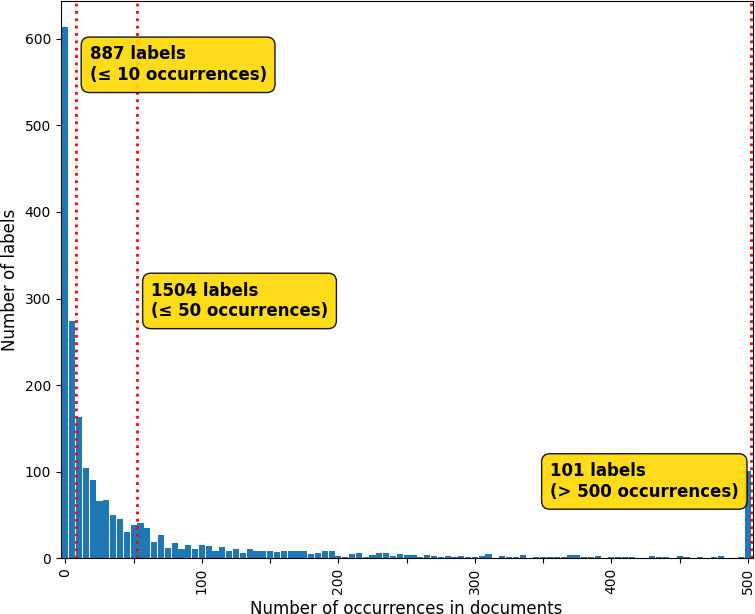
\includegraphics[width=7.5cm]{Images/ivacic.label_dist_newsmon_sr-2.png}}
%\hfill
\subfloat[\centering]{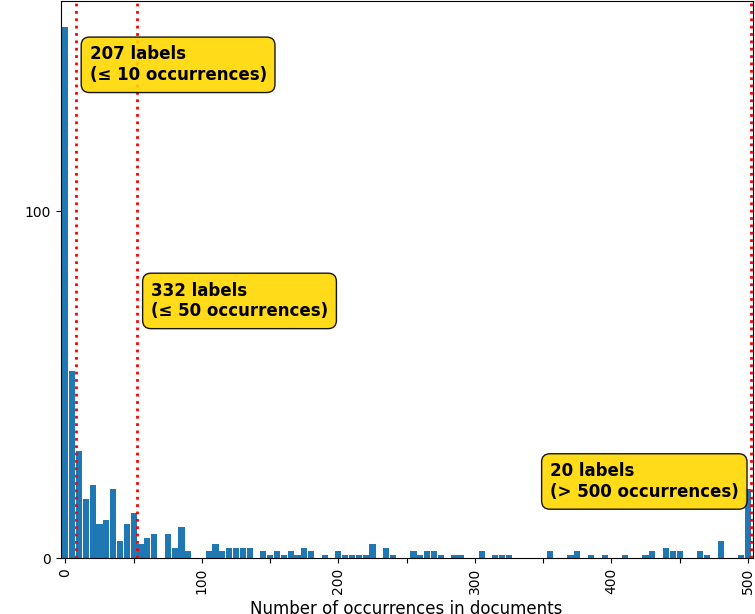
\includegraphics[width=7.5cm]{Images/ivacic.label_dist_newsmon_mk-2.png}}\\
%\isPreprints{}{% This command is only used for ``preprints''.
\end{adjustwidth}
%} % If the paper is ``preprints'', please uncomment this parenthesis.
\caption{(\textbf{a}) The distribution of label occurrences in the NewsMon\textsubscript{sr} dataset. (\textbf{b}) The distribution of label occurrences in the NewsMon\textsubscript{mk} dataset. 
\label{fig:sr_mk_dataset_statistics}}
\end{figure}
\vspace{-6pt}
 \begin{table}[H]
   % \centering
\small
    \caption{NewsMon\textsubscript{sr} (all labels): micro/macro F1, P, R, and~subset accuracy for SVM and logistic regression (OvA TF-IDF), BGE-M3, and~fine-tuned BGE-M3 under zero-shot and~RAE-XMC.}
%    \resizebox{0.65\textwidth}{!}{
%    \setlength{\tabcolsep}{3pt}
    \begin{tabularx}{\textwidth}{l l C c C c C c C}
        \toprule
        \multicolumn{1}{c}{\textbf{Model}} & 
        \multicolumn{1}{c}{\textbf{Method}} & 
        \multicolumn{1}{c}{\(\boldsymbol{\upmu}\)\textbf{F1}} &
        \multicolumn{1}{c}{\(\boldsymbol{\upmu}\)\textbf{P}} &
        \multicolumn{1}{c}{\(\boldsymbol{\upmu}\)\textbf{R}} &
        \multicolumn{1}{c}{\textbf{F1}} &
        \multicolumn{1}{c}{\textbf{P}} &
        \multicolumn{1}{c}{\textbf{R}} &
        \multicolumn{1}{c}{\textbf{Acc}} \\
        \midrule
      
        SVM    & OVA-TFIDF    & \textbf{69.15} & 76.45 & 63.13 & 33.43 & 39.26 & 30.97 & 44.80 \\
        LogReg & OVA-TFIDF    & 68.70 & \underline{77.54} & 61.66 & 32.61 & \underline{39.64} & 29.51 & 44.67 \\
        \midrule
        BGE-M3 & zshot        & 63.71 & 61.93 & \underline{65.59} & 33.72 & 33.48 & \underline{36.40} & 45.04 \\
        BGE-M3 & RAE-XMC      & \underline{68.86} & 76.85 & 62.38 & \underline{34.40} & 39.41 & 32.70 & \underline{47.92} \\
        \midrule
        FT-BGE\textsubscript{sl} & zshot        & 65.65 & 65.07 & \textbf{66.23} & \textbf{35.19} & 35.73 & \textbf{37.22} & 46.33 \\
        FT-BGE\textsubscript{sl} & RAE-XMC      & 68.62 & \textbf{82.64} & 58.66 & 33.50 & \textbf{39.69} & 31.05 & \textbf{48.98} \\
        \bottomrule
    \end{tabularx}
        \footnotesize {\textbf{Note:} Best results are shown in \textbf{bold}, and~second-best results are \underline{underlined}.}
   % }
    \label{tab:result_serbian_all}
\end{table}

\subsection[\appendixname~\thesubsection]{Preliminary Experimental Results}
\label{subsec:sr_mk_results}
We report preliminary results for NewsMon\textsubscript{sr} and NewsMon\textsubscript{mk} in \mbox{Tables~\ref{tab:result_serbian_all} and \ref{tab:result_macedonian_all},} respectively. The~XLM-R baseline is not included in this release. As~summarised in \cref{tab:factor_attribution_appendix}, RAE-XMC contributes the largest single share of the gains, especially for subset accuracy (+2.88\,pp on NewsMon\textsubscript{sr}, +4.00\,pp on NewsMon\textsubscript{mk}). 
At the same time, hard-negative fine-tuning adds complementary improvements in micro-F1 (+1.94\,pp on NewsMon\textsubscript{sr}, +3.56\,pp on NewsMon\textsubscript{mk}). 
The small negative interaction terms suggest partial redundancy between the two components, yet the combined effect remains clearly positive overall (+4.90\,pp and +5.96\,pp in $\mu$F1 for NewsMon\textsubscript{sr} and NewsMon\textsubscript{mk}, respectively). 
Importantly, the~HN–fine-tuned encoder (FT-BGE\textsubscript{sl}) was transferred from Slovenian rather than tuned on Serbian or Macedonian; therefore, these effects reflect cross-lingual transfer and can diverge from the main, language-specific results, where the HN fine-tuning was the highest contributor. 
Consequently, factor attribution and classification performance figures should be interpreted as provisional, reflecting cross-lingual transfer rather than language-specific~optimisation.


\begin{table}[H]
    \small
    \caption{NewsMon\textsubscript{mk} (all labels): micro/macro F1, P, R, and~subset accuracy for SVM and logistic regression (OvA TF-IDF), BGE-M3, and~fine-tuned BGE-M3 under zero-shot and~RAE-XMC.}
%    \resizebox{0.65\textwidth}{!}{
%    \setlength{\tabcolsep}{3pt}
    \begin{tabularx}{\textwidth}{l l C c C c C c C}
        \toprule
        \multicolumn{1}{c}{\textbf{Model}} & 
        \multicolumn{1}{c}{\textbf{Method}} & 
        \multicolumn{1}{c}{\(\boldsymbol{\upmu}\)\textbf{F1}} &
        \multicolumn{1}{c}{\(\boldsymbol{\upmu}\)\textbf{P}} &
        \multicolumn{1}{c}{\(\boldsymbol{\upmu}\)\textbf{R}} &
        \multicolumn{1}{c}{\textbf{F1}} &
        \multicolumn{1}{c}{\textbf{P}} &
        \multicolumn{1}{c}{\textbf{R}} &
        \multicolumn{1}{c}{\textbf{Acc}} \\
        \midrule
        
        SVM    & OVA-TFIDF    & \underline{81.72} & 87.67 & 76.53 & \underline{46.07} & \underline{49.96} & 44.14 & 49.43 \\
        LogReg & OVA-TFIDF    & 80.98 & \underline{88.38} & 74.72 & 44.23 & 49.46 & 41.64 & 47.71 \\
        \midrule
        BGE-M3 & zshot        & 76.72 & 74.62 & \underline{78.95} & 44.67 & 44.28 & \underline{46.80} & 47.14 \\
        BGE-M3 & RAE-XMC      & 80.45 & 85.81 & 75.72 & 43.39 & 47.33 & 41.92 & \underline{51.14} \\
        \midrule
        FT-BGE\textsubscript{sl} & zshot        & 80.29 & 79.48 & \textbf{81.11} & \textbf{47.95} & 47.74 & \textbf{49.34} & 49.02 \\
        FT-BGE\textsubscript{sl} & RAE-XMC      & \textbf{82.68} & \textbf{90.56} & 76.06 & 45.17 & \textbf{50.13} & 42.97 & \textbf{51.63} \\
       \bottomrule
    \end{tabularx}
        \footnotesize {\textbf{Note:} Best results are shown in \textbf{bold}, and~second-best results are \underline{underlined}.}
  %  }
    \label{tab:result_macedonian_all}
\end{table}
\vspace{-6pt}
\begin{table}[H]
    \small
    \caption{Factor attribution (absolute \%-point deltas) for Serbian (\textit{NewsMon\textsubscript{sr}}) and Macedonian (\textit{NewsMon\textsubscript{mk}}) datasets. 
    Effects correspond to hard-negative fine-tuning (HN), RAE-XMC retrieval, and~their interaction.}
%    \resizebox{0.95\textwidth}{!}{
%    \setlength{\tabcolsep}{3pt}
  
\begin{adjustwidth}{-\extralength}{0cm}
%\centering %% If there is a figure in wide page, please release command \centering
  \begin{tabularx}{\fulllength}{l C c C c C c C c}
        \toprule
        \multicolumn{1}{c}{\textbf{Dataset}} &
        \multicolumn{1}{c}{\(\Delta\)\(\boldsymbol{\upmu}\)\textbf{F1 HN}} &
        \multicolumn{1}{c}{\(\Delta\)\(\boldsymbol{\upmu}\)\textbf{F1 RAE}} &
        \multicolumn{1}{c}{\(\Delta\)\(\boldsymbol{\upmu}\)\textbf{F1 Int.}} &
        \multicolumn{1}{c}{\(\Delta\)\(\boldsymbol{\upmu}\)\textbf{F1 Total}} &
        \multicolumn{1}{c}{\(\Delta\)\textbf{Acc HN}} &
        \multicolumn{1}{c}{\(\Delta\)\textbf{Acc RAE}} &
        \multicolumn{1}{c}{\(\Delta\)\textbf{Acc Int.}} &
        \multicolumn{1}{c}{\(\Delta\)\textbf{Acc Total}} \\
        \midrule
        
        NewsMon\textsubscript{sr}  & +1.94 & +5.15 & $-$2.18 & +4.90 & +1.29 & +2.88 & $-$0.23 & +3.95 \\
        NewsMon\textsubscript{mk}  & +3.56 & +3.72 & $-$1.33 & +5.96 & +1.88 & +4.00 & $-$1.39 & +4.49 \\
        \bottomrule
        
    \end{tabularx}
\end{adjustwidth}
            \footnotesize {\textbf{Note:} “HN” = hard-negative fine-tuning effect (FT-BGE zero-shot – BGE-M3 zero-shot); “RAE” = RAE-XMC retrieval effect (BGE-M3 RAE – BGE-M3 zero-shot); “Int.” = interaction term explaining residual; “Total” = overall delta from BGE-M3 zero-shot → FT-BGE RAE-XMC. Values derived from \cref{tab:result_serbian_all,tab:result_macedonian_all}.
        }
  %  }
    \label{tab:factor_attribution_appendix}
\end{table}


\section[\appendixname~\thesection]{The Original RAE-XMC Framework}
\label{sec:raexmc_model}
\begin{figure}[H]
%  \centering
  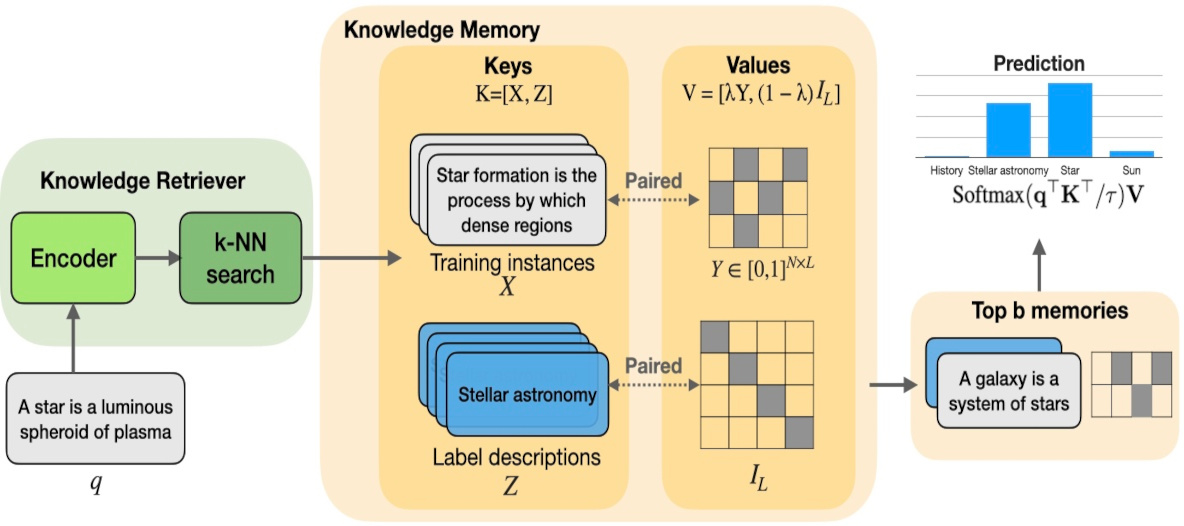
\includegraphics[width=0.9\textwidth]{Images/wang.raexmc_model.jpeg}
  \caption{
  Original RAE-XMC framework. Reproduced from
  Wang, Y.-S., Chang, W.-C., Jiang, J.-Y., Zhang, J., Yu, H.-F., \& Vishwanathan, S. V. N. (2025),
  \textit{Retrieval-augmented Encoders for Extreme Multi-label Text Classification}~\citep{wang2025retrievalaugmentedencodersextrememultilabel},
  arXiv:2502.10615. Licensed under \href{https://creativecommons.org/licenses/by/4.0/}{CC BY 4.0}.
  Changes: [resized; otherwise “no changes”].}
  \label{fig:rae_xmc_framework}
\end{figure}


\section[\appendixname~\thesection]{Hyperparameters}
\label{sec:hyper_parameters}
\subsection[\appendixname~\thesubsection]{SVM Hyperparameters}
\label{subsec:hyper_parameters_svm}
C-Support Vector Classification was used for the SVM classifier, implemented by the RAPIDS cuML library \citep{raschka2020machine} with the Scikit-learn~\citep{scikit-learn} multi-target classification strategy consisting of fitting one classifier per target, where for the SVC we~used:
\begin{itemize}\itemsep=0pt
  \item Radial basis function (RBF) kernel,
  \item Regularisation parameter ($C$) was set to 10,000 for NewsMon\textsubscript{sl} and 10 for EURLEX57K.
  \item Gamma coefficient for RBF was set to 0.001 for NewsMon\textsubscript{sl} and 1.0 for EURLEX57K.
  \item Maximum term document frequency was set to 0.8 for NewsMon\textsubscript{sl} and 1.0\linebreak for EURLEX57K.
\end{itemize}

The hyperparameters were obtained through a grid search using Scikit-learn.
Due to the high memory consumption of the SVM classification, which exceeded the available hardware when all classifiers were trained simultaneously, we partitioned the label space into batches of 240 to maintain memory usage below 16 GB during both training and evaluation. For~the TF-IDF representation, we used \mbox{Scikit-learn's} \mbox{TfidfVectorizer} with a maximum of 10,000~features.

\subsection[\appendixname~\thesubsection]{Logistic Regression Hyperparameters}
\label{subsec:hyper_parameters_logreg}
We used the same libraries and strategy as for SVM for the logistic regression model with the best~hyperparameters:
\begin{itemize}\itemsep=0pt
  \item L2 penalty,
  \item Tolerance for stopping criteria: 0.0001,
  \item Inverse of regularisation strength ($C$) set to 1000 for NewsMon\textsubscript{sl} and 10\linebreak for EURLEX57K.
  \item Maximum term document frequency was set to 0.8 for NewsMon\textsubscript{sl} and EURLEX57K.
\end{itemize}

For both SVM and Logistic regression, we used a single consumer-grade GPU (Nvidia GeForce 4070 Ti Super).

\subsection[\appendixname~\thesubsection]{XLM-RoBERTa-Base Fine-Tuning Hyperparameters}
\label{subsec:hyper_parameters_xlmr}
For the baseline training, we did not perform hyperparameter optimisation; all the models were fine-tuned using the default set of hyperparameters from HuggingFace's Transformers library~\citep{wolf-etal-2020-transformers}, optimised for a large selection of common NLP~tasks:
\begin{itemize}\itemsep=0pt
  \item AdamW optimiser with a learning rate of 3 $\times$ 10\textsuperscript{$-5$}.
  \item Weight decay set to 0.01 for regularisation.
  \item Training for a maximum of 30 epochs.
  \item Batch size of 16.
  \item Maximum length of 512 sub-word tokens.
  \item 30 epochs.
  \item Best model selection based on the validation set micro F1-score.
\end{itemize}

We used a single consumer-grade GPU (NVIDIA GeForce 4070 Ti Super).

\subsection[\appendixname~\thesubsection]{BGE-M3 Fine-Tuning Hyperparameters}
\label{subsec:hyper_parameters_bge_m3}
BGE-M3 models were fine-tuned using the default set of hyperparameters from the FlagEmbedding~library:
\begin{itemize}\itemsep=0pt
  \item AdamW optimiser with a learning rate of 1 $\times$ 10\textsuperscript{$-5$}.
  \item Train group size of 4.
  \item Batch size of 2.
  \item Maximum length of 4096 sub-word tokens for query and passage.
  \item Temperature 0.02.
  \item 20 epochs.
  \item Precision fp16.
\end{itemize}

We used a single data centre GPU (NVIDIA A100).

\subsection[\appendixname~\thesubsection]{Retrieval Model Hyperparameter Search}
\label{subsec:hyper_parameter_search}

We ran a hyperparameter search for 1,000 trials, searching for the best $top\mhyphen k \in [10, 100]$, temperature $\tau \in [0.01, 0.1]$, and~$\lambda \in [0.1, 1.0]$ parameters, maximising the subset~accuracy.

\begin{table}[H]
    %\centering
    \caption{RAE-XMC Hyperparameter search~results.}
%    \resizebox{0.45\textwidth}{!}{
    \begin{tabularx}{\textwidth}{L L CCC}
        \toprule
        \textbf{Model} & \textbf{Dataset} & \(\mathbf{Top\mhyphen k}\) & \(\boldsymbol{\tau}\) & \(\boldsymbol{\lambda}\) \\
        \midrule
       
        BGE-M3 & EURLEX57K & 10 & 0.031 & 0.998 \\
        BGE-M3 & NewsMon & 16 & 0.091 & 0.999 \\
        \midrule
        FT-BGE & EURLEX57K & 69 & 0.031 & 1.000 \\
        FT-BGE & NewsMon & 13 & 0.098 & 0.816 \\
        \bottomrule
    \end{tabularx}
   % }
\end{table}


\section[\appendixname~\thesection]{Evaluation Metrics}
\label{sec:evaluation_metrics}
In this section, we use $N$ for the number of test samples, $L$ for the number of labels, $y_i$ for an individual example label set, and~$\hat{y_i}$ for the predicted example label~set.
\subsection[\appendixname~\thesubsection]{Example-Based Evaluation Metrics}
For the example-based evaluation, we used subset accuracy:
\begin{equation}
  Accuracy = \frac{1}{N}\sum_{i=1}^{N}I( y_i = \hat{y_i})
\end{equation}
where  $I(true) = 1$ and $I(false) = 0$

\subsection[\appendixname~\thesubsection]{Label-based Evaluation Metrics}
%For the label-based macro-averaged evaluation %\hl{Macro-averaged metrics could not be computed in cases where true positives (TP), false negatives (FN), and~false positives (FP) were all zero for a given label. In~such cases, a~value of zero was used in the averaging computation}, %MDPI: Footnote is not allowed for this journal. We moved it here. Please confirm.
%AUTHORS: We confirm.
For the label‑based macro‑averaged evaluation, metrics are undefined when true positives (TP), false negatives (FN), and false positives (FP) are all zero for a label; in such cases, we assign a value of zero to that label in the macro average. We used:
\begin{equation}
  Precision_{macro} = \frac{1}{L}\sum_{i=1}^{L}\frac{TP_i}{TP_i + FP_i}
\end{equation}
\begin{equation}
  Recall_{macro} = \frac{1}{L}\sum_{i=1}^{L}\frac{TP_i}{TP_i + FN_i}
\end{equation}
%Macro-averaged metrics could not be computed in cases where true positives (TP), false negatives (FN), and~false positives (FP) were all zero for a given label. In~such cases, a~value of zero was used in the averaging computation

For the label-based micro-averaged evaluation, we used:
\begin{equation}
  Precision_{micro} = \frac{\sum_{i=1}^{L} TP_i}{\sum_{i=1}^{L} (TP_i + FP_i)}
\end{equation}
\begin{equation}
  Recall_{micro} = \frac{\sum_{i=1}^{L} TP_i}{\sum_{i=1}^{L} (TP_i + FN_i)}
\end{equation}

In both cases, $F_1\mhyphen score$ can be computed as follows:
\begin{equation}
  F_1\mhyphen score = 2  \cdot \frac{Precision \cdot Recall}{Precision +  Recall}
\end{equation}


%%%%%%%%%%%%%%%%%%%%%%%%%%%%%%%%%%%%%%%%%%
%\isPreprints{}{% This command is only used for ``preprints''.
\begin{adjustwidth}{-\extralength}{0cm}
%} % If the paper is ``preprints'', please uncomment this parenthesis.
%\printendnotes[custom] % Un-comment to print a list of endnotes

\reftitle{References}
% Please provide either the correct journal abbreviation (e.g. according to the “List of Title Word Abbreviations” http://www.issn.org/services/online-services/access-to-the-ltwa/) or the full name of the journal.
% Citations and References in Supplementary files are permitted provided that they also appear in the reference list here. 

%=====================================
% References, variant A: external bibliography
%=====================================
% \bibliography{your_external_BibTeX_file}
%\bibliography{bibliography}
\begin{thebibliography}{999}

\bibitem[Rupnik et~al.(2016)Rupnik, Muhic, Leban, Skraba, Fortuna, and
  Grobelnik]{rupnik2016news}
Rupnik, J.; Muhic, A.; Leban, G.; Skraba, P.; Fortuna, B.; Grobelnik, M.
\newblock News across languages-cross-lingual document similarity and event
  tracking.
\newblock {\em J. Artif. Intell. Res.} {\bf 2016}, {\em
  55},~283--316.

\bibitem[Zhang et~al.(2022)Zhang, Guo, Shen, and Han]{zang2022event_detection}
Zhang, Y.; Guo, F.; Shen, J.; Han, J.
\newblock Unsupervised Key Event Detection from Massive Text Corpora.
\newblock In Proceedings of the 28th ACM SIGKDD Conference
  on Knowledge Discovery and Data Mining, KDD '22, Washington, DC, USA, 14--18 August
 2022; pp.
  2535--2544.
\newblock {\url{https://doi.org/10.1145/3534678.3539395}}.

\bibitem[Yoon et~al.(2023)Yoon, Lee, Zhang, and Han]{yoon2023story_detection}
Yoon, S.; Lee, D.; Zhang, Y.; Han, J.
\newblock Unsupervised Story Discovery from Continuous News Streams via
  Scalable Thematic Embedding.
\newblock In Proceedings of the 46th International ACM SIGIR
  Conference on Research and Development in Information Retrieval, SIGIR '23, Taipei Taiwan, 23--27 July 2023; pp. 802--811.
\newblock {\url{https://doi.org/10.1145/3539618.3591782}}.

\bibitem[Devlin et~al.(2019)Devlin, Chang, Lee, and Toutanova]{devlin2018bert}
Devlin, J.; Chang, M.W.; Lee, K.; Toutanova, K.
\newblock {BERT}: Pre-training of Deep Bidirectional Transformers for Language
  Understanding.
\newblock In Proceedings of the 2019 Conference of the North
  {A}merican Chapter of the Association for Computational Linguistics: Human
  Language Technologies, Volume 1 (Long and Short Papers), Minneapolis, 
  MN, USA, 2--7 June 2019; pp. 4171--4186.
  %AUTHORS: We confirm.
\newblock {\url{https://doi.org/10.18653/v1/N19-1423}}.

\bibitem[Raffel et~al.(2020)Raffel, Shazeer, Roberts, Lee, Narang, Matena,
  Zhou, Li, and Liu]{raffel2020exploring}
Raffel, C.; Shazeer, N.; Roberts, A.; Lee, K.; Narang, S.; Matena, M.; Zhou,
  Y.; Li, W.; Liu, P.J.
\newblock Exploring the Limits of Transfer Learning with a Unified Text-to-Text
  Transformer. \emph{arXiv}  \textbf{2020}, arXiv:1910.10683.
\bibitem[Brown et~al.(2020)Brown, Mann, Ryder, Subbiah, Kaplan, Dhariwal,
  Neelakantan, Shyam, Sastry, Askell, Agarwal, Herbert{-}Voss, Krueger,
  Henighan, Child, Ramesh, Ziegler, Wu, Winter, Hesse, Chen, Sigler, Litwin,
  Gray, Chess, Clark, Berner, McCandlish, Radford, Sutskever, and
  Amodei]{brown2020language}
Brown, T.B.; Mann, B.; Ryder, N.; Subbiah, M.; Kaplan, J.; Dhariwal, P.;
  Neelakantan, A.; Shyam, P.; Sastry, G.; Askell, A.;  et~al.
\newblock Language Models are Few-Shot Learners.
\newblock In Proceedings of the Advances in Neural Information Processing
  Systems 33: Annual Conference on Neural Information Processing Systems 2020,
  NeurIPS 2020, Virtual, 6--12 December 2020.
\bibitem[Touvron et~al.(2023)Touvron, Martin, Stone, Albert, Almahairi, Babaei,
  Bashlykov, Batra, Bhargava, Bhosale, Bikel, Blecher, Ferrer, Chen, Cucurull,
  Esiobu, Fernandes, Fu, Fu, Fuller, Gao, and
  \dots]{touvron2023llama2openfoundation}
Touvron, H.; Martin, L.; Stone, K.; Albert, P.; Almahairi, A.; Babaei, Y.;
  Bashlykov, N.; Batra, S.; Bhargava, P.; Bhosale, S.;  et~al.
\newblock Llama 2: Open Foundation and Fine-Tuned Chat Models.
\newblock {\em arXiv } {\bf 2023}, arXiv:2307.09288.

\bibitem[Tarekegn et~al.(2024)Tarekegn, Ullah, and
  Cheikh]{tarekegn2024deeplearningmultilabellearning}
Tarekegn, A.N.; Ullah, M.; Cheikh, F.A.
\newblock Deep Learning for Multi-Label Learning: A Comprehensive Survey.
\newblock {\em arXiv} {\bf 2024}, arXiv:2401.16549.

\bibitem[Li et~al.(2022)Li, Peng, Li, Xia, Yang, Sun, Yu, and
  He]{li2022surveytextclassification}
Li, Q.; Peng, H.; Li, J.; Xia, C.; Yang, R.; Sun, L.; Yu, P.S.; He, L.
\newblock A Survey on Text Classification: From Traditional to Deep Learning.
\newblock {\em ACM Trans. Intell. Syst. Technol.} {\bf 2022}, {\em 13}, 1--41.
\newblock {\url{https://doi.org/10.1145/3495162}}.

\bibitem[Dubey et~al.(2024)Dubey, Jauhri, Pandey, Kadian, Al-Dahle, Letman,
  Mathur, Schelten, Yang, Fan, Goyal, Hartshorn, Yang, Mitra, Sravankumar,
  Korenev, Hinsvark, Rao, Zhang, Rodriguez, Gregerson, and
  \dots]{dubey2024llama3herdmodels}
Dubey, A.; Jauhri, A.; Pandey, A.; Kadian, A.; Al-Dahle, A.; Letman, A.;
  Mathur, A.; Schelten, A.; Yang, A.; Fan, A.;  et~al.
\newblock The Llama 3 Herd of Models.
\newblock {\em arXiv} {\bf 2024}, arXiv:2407.21783.

\bibitem[OpenAI et~al.(2023)OpenAI, Achiam, Adler, Agarwal, Ahmad, Akkaya,
  Aleman, Almeida, Altenschmidt, Altman, Anadkat, Avila, Babuschkin, Balaji,
  Balcom, Baltescu, Bao, Bavarian, Belgum, Bello, and
  \dots]{openai2024gpt4technicalreport}
OpenAI; Achiam, J.; Adler, S.; Agarwal, S.; Ahmad, L.; Akkaya, I.; Aleman,
  F.L.; Almeida, D.; Altenschmidt, J.; Altman, S.;  et~al.
\newblock GPT-4 Technical Report.
\newblock {\em arXiv} {\bf 2023}, arXiv:2303.08774.

\bibitem[Team et~al.(2023)Team, Anil, Borgeaud, Alayrac, Yu, Soricut,
  Schalkwyk, Dai, Hauth, Millican, Silver, Johnson, Antonoglou, Schrittwieser,
  Glaese, Chen, Pitler, Lillicrap, Lazaridou, Firat, and
  \dots]{geminiteam2024geminifamilyhighlycapable}
Team, G.; Anil, R.; Borgeaud, S.; Alayrac, J.B.; Yu, J.; Soricut, R.;
  Schalkwyk, J.; Dai, A.M.; Hauth, A.; Millican, K.;  et~al.
\newblock Gemini: A Family of Highly Capable Multimodal Models.
\newblock {\em arXiv} {\bf 2023}, arXiv:2312.11805.

\bibitem[Abdin et~al.(2024)Abdin, Aneja, Behl, Bubeck, Eldan, Gunasekar,
  Harrison, Hewett, Javaheripi, Kauffmann, Lee, Lee, Li, Liu, Mendes, Nguyen,
  Price, de~Rosa, Saarikivi, Salim, Shah, Wang, Ward, Wu, Yu, Zhang, and
  Zhang]{abdin2024phi4technicalreport}
Abdin, M.; Aneja, J.; Behl, H.; Bubeck, S.; Eldan, R.; Gunasekar, S.; Harrison,
  M.; Hewett, R.J.; Javaheripi, M.; Kauffmann, P.;  et~al.
\newblock Phi-4 Technical Report.
\newblock {\em arXiv} {\bf 2024}, arXiv:2412.08905.

\bibitem[Team(2025{\natexlab{a}})]{gemma_2025}
Team, G.; Kamath, A.; Ferret, J.; Pathak, S.; Vieillard, N.; Merhej, R.; Perrin, S.; Matejovicova, T.; Ramé, A.; Rivière, M.; et al.
\newblock Gemma 3 technical report. \emph{arXiv} {\bf 2025}, arXiv:2503.19786.

%\bibitem[Team(2025{\natexlab{b}})]{qwq32b}
%Team, Q.
%\newblock QwQ-32B: Embracing the Power of Reinforcement Learning. \hl{ 2025.} %MDPI: Please provide more information about the article type, such as book (please provide the name and location of the publisher); online resource (please provide the URL of the website and the date it was accessed (Date Month Year)); or journal article (please provide the name of the journal, the year and volume in which it was published, and the page number). Please refer to https://www.mdpi.com/authors/references for full reference formatting guides.
%AUTHORS: We decided to drop this reference (It was an example of an RL-type SLM decoder, but in the context used, the reference was not that important - we already have two references which are better suited) 

\bibitem[Subramanian et~al.(2025)Subramanian, Elango, and
  Gungor]{subramanian2025smalllanguagemodelsslms}
Subramanian, S.; Elango, V.; Gungor, M.
\newblock Small Language Models (SLMs) Can Still Pack a Punch: A survey.
\newblock {\em arXiv } {\bf 2025}, arXiv:2501.05465.

\bibitem[Vajjala and Shimangaud(2025)]{vajjala2025textclassificationllmera}
Vajjala, S.; Shimangaud, S.
\newblock Text Classification in the LLM Era---Where do we stand?
\newblock {\em arXiv} {\bf 2025}, arXiv:2502.11830.

\bibitem[Muralidharan et~al.(2024)Muralidharan, Sreenivas, Joshi, Chochowski,
  Patwary, Shoeybi, Catanzaro, Kautz, and Molchanov]{muralidharan2024compact}
Muralidharan, S.; Sreenivas, S.T.; Joshi, R.; Chochowski, M.; Patwary, M.;
  Shoeybi, M.; Catanzaro, B.; Kautz, J.; Molchanov, P.
\newblock Compact Language Models via Pruning and Knowledge Distillation.
\newblock {\em arXiv} {\bf 2024}, arXiv:2407.14679.

\bibitem[Gu et~al.(2023)Gu, Dong, Wei, and
  Huang]{gu2024minillmknowledgedistillationlarge}
Gu, Y.; Dong, L.; Wei, F.; Huang, M.
\newblock MiniLLM: Knowledge Distillation of Large Language Models.
\newblock {\em arXiv} {\bf 2023}, arXiv:2306.08543.

\bibitem[Malinovskii et~al.(2024)Malinovskii, Mazur, Ilin, Kuznedelev,
  Burlachenko, Yi, Alistarh, and
  Richtarik]{malinovskii2024pvtuningstraightthroughestimationextreme}
Malinovskii, V.; Mazur, D.; Ilin, I.; Kuznedelev, D.; Burlachenko, K.; Yi, K.;
  Alistarh, D.; Richtarik, P.
\newblock PV-Tuning: Beyond Straight-Through Estimation for Extreme LLM
  Compression.
\newblock {\em arXiv} {\bf 2024}, arXiv:2405.14852.

\bibitem[Kuzman and Ljubešić(2025)]{kuzman2025LLMteacher}
Kuzman, T.; Ljubešić, N.
\newblock LLM Teacher-Student Framework for Text Classification With No
  Manually Annotated Data: A Case Study in IPTC News Topic Classification.
\newblock {\em IEEE Access} {\bf 2025}, {\em 13},~35621--35633.
\newblock {\url{https://doi.org/10.1109/ACCESS.2025.3544814}}.

\bibitem[Dasgupta et~al.(2023)Dasgupta, Lamba, Kushwaha, Ravish, Katyan, Das,
  and Kumar]{dasgupta2025reviewextrememultilabelclassification}
Dasgupta, A.; Lamba, P.; Kushwaha, A.; Ravish, K.; Katyan, S.; Das, S.; Kumar,
  P.
\newblock Review of Extreme Multilabel Classification.
\newblock {\em arXiv} {\bf 2023}, arXiv:2302.05971.

\bibitem[Wang et~al.(2025)Wang, Chang, Jiang, Zhang, Yu, and
  Vishwanathan]{wang2025retrievalaugmentedencodersextrememultilabel}
Wang, Y.S.; Chang, W.C.; Jiang, J.Y.; Zhang, J.; Yu, H.F.; Vishwanathan, S.V.N.
\newblock Retrieval-augmented Encoders for Extreme Multi-label Text
  Classification.
\newblock {\em arXiv} {\bf 2025}, arXiv:2502.10615.

\bibitem[Dai et~al.(2022)Dai, Chalkidis, Darkner, and
  Elliott]{dai2022revisitingtransformer}
Dai, X.; Chalkidis, I.; Darkner, S.; Elliott, D.
\newblock Revisiting Transformer-based Models for Long Document Classification.
\newblock In Proceedings of the Findings of the Association for Computational
  Linguistics: EMNLP 2022, Abu Dhabi, United Arab Emirates, 7--11 December 2022; pp. 7212--7230.
\newblock {\url{https://doi.org/10.18653/v1/2022.findings-emnlp.534}}.
%AUTHORS: We confirm.

\bibitem[Duan et~al.(2022)Duan, You, Wu, and Sun]{duan2022fusiontwostream}
Duan, L.; You, Q.; Wu, X.; Sun, J.
\newblock Multilabel Text Classification Algorithm Based on Fusion of
  Two-Stream Transformer.
\newblock {\em Electronics} {\bf 2022}, {\em 11}, 2138.
\newblock {\url{https://doi.org/10.3390/electronics11142138}}.

\bibitem[Liu et~al.(2022)Liu, Liu, Cao, and Du]{liu2022cnle}
Liu, M.; Liu, L.; Cao, J.; Du, Q.
\newblock Co-attention network with label embedding for text classification.
\newblock {\em Neurocomputing} {\bf 2022}, {\em 471},~61--69.
\newblock {\url{https://doi.org/10.1016/j.neucom.2021.10.099}}.
%AUTHORS: We confirm - fixing link.

\bibitem[Yarullin and Serdyukov(2021)]{yarullin2020bertforseq}
Yarullin, R.; Serdyukov, P.
\newblock BERT for Sequence-to-Sequence Multi-label Text Classification.
\newblock In \emph{Analysis of Images, Social Networks and Texts};
  van~der Aalst, W.M.P., Batagelj, V., Ignatov, D.I., Khachay, M., Koltsova,
  O., Kutuzov, A., Kuznetsov, S.O., Lomazova, I.A., Loukachevitch, N., Napoli,
  A.,  et~al., Eds.; Springer: Cham, Switzerland, 2021; pp. 187--198.
\newblock {\url{https://doi.org/10.1007/978-3-030-72610-2_14}}.

\bibitem[Fallah et~al.(2023)Fallah, Bruno, Bellot, and
  Murisasco]{fallah2023exploitinglabeldependencies}
Fallah, H.; Bruno, E.; Bellot, P.; Murisasco, E.
\newblock Exploiting Label Dependencies for Multi-Label Document Classification
  Using Transformers.
\newblock In Proceedings of the ACM Symposium on Document
  Engineering 2023, DocEng '23, Limerick, Ireland, 22--25 August 2023. 
\newblock {\url{https://doi.org/10.1145/3573128.3609356}}.

\bibitem[Li et~al.(2024)Li, Chen, and Zeng]{li2024kenet}
Li, B.; Chen, Y.; Zeng, L.
\newblock Kenet:Knowledge-Enhanced DOC-Label Attention Network for Multi-Label
  Text Classification.
\newblock In Proceedings of the ICASSP 2024---2024 IEEE International
  Conference on Acoustics, Speech and Signal Processing (ICASSP), Seoul, Republic of Korea, 14--19 April 2024; pp.
  11961--11965.
\newblock {\url{https://doi.org/10.1109/ICASSP48485.2024.10447643}}.

\bibitem[Sennrich et~al.(2016)Sennrich, Haddow, and
  Birch]{sennrich2016bpeusage}
Sennrich, R.; Haddow, B.; Birch, A.
\newblock Neural Machine Translation of Rare Words with Subword Units.
\newblock In Proceedings of the 54th Annual Meeting of the
  Association for Computational Linguistics (Volume 1: Long Papers), Berlin,
  Germany, 7--12 August 2016; pp. 1715--1725.
\newblock {\url{https://doi.org/10.18653/v1/P16-1162}}.

\bibitem[Kudo and Richardson(2018)]{kudo-richardson2018sentencepiece}
Kudo, T.; Richardson, J.
\newblock {S}entence{P}iece: A simple and language independent subword
  tokenizer and detokenizer for Neural Text Processing.
\newblock In Proceedings of the 2018 Conference on Empirical
  Methods in Natural Language Processing: System Demonstrations, Brussels,
  Belgium, 31 October--4 November 2018; pp. 66--71.
\newblock {\url{https://doi.org/10.18653/v1/D18-2012}}.

\bibitem[Vaswani et~al.(2017)Vaswani, Shazeer, Parmar, Uszkoreit, Jones, Gomez,
  Kaiser, and Polosukhin]{vaswani2017attention}
Vaswani, A.; Shazeer, N.; Parmar, N.; Uszkoreit, J.; Jones, L.; Gomez, A.N.;
  Kaiser, L.; Polosukhin, I.
\newblock Attention is All You Need.
\newblock In Proceedings of the Advances in Neural Information Processing
  Systems 30: Annual Conference on Neural Information Processing Systems 2017, Long Beach, CA, USA,
  4--9 December 2017;
 pp. 5998--6008.

\bibitem[Park et~al.(2022)Park, Vyas, and Shah]{park2022efficient}
Park, H.; Vyas, Y.; Shah, K.
\newblock Efficient Classification of Long Documents Using Transformers.
\newblock In Proceedings of the 60th Annual Meeting of the
  Association for Computational Linguistics (Volume 2: Short Papers), Dublin, Ireland, 22--27 May 2022; pp. 702--709.
\newblock {\url{https://doi.org/10.18653/v1/2022.acl-short.79}}.

\bibitem[Beltagy et~al.(2020)Beltagy, Peters, and
  Cohan]{beltagy2020longformerlongdocumenttransformer}
Beltagy, I.; Peters, M.E.; Cohan, A.
\newblock Longformer: The Long-Document Transformer.
\newblock {\em arXiv} {\bf 2020}, arXiv:2004.05150.

\bibitem[Zaheer et~al.(2020)Zaheer, Guruganesh, Dubey, Ainslie, Alberti,
  Ontanon, Pham, Ravula, Wang, Yang, and Ahmed]{zaheer2021bigbird}
Zaheer, M.; Guruganesh, G.; Dubey, A.; Ainslie, J.; Alberti, C.; Ontanon, S.;
  Pham, P.; Ravula, A.; Wang, Q.; Yang, L.;  et~al.
\newblock Big Bird: Transformers for Longer Sequences.
\newblock {\em arXiv} {\bf 2020}, arXiv:2007.14062.

\bibitem[Ding et~al.(2020)Ding, Zhou, Yang, and Tang]{ding2020cogltx}
Ding, M.; Zhou, C.; Yang, H.; Tang, J.
\newblock CogLTX: Applying {BERT} to Long Texts.
\newblock In Proceedings of the Advances in Neural Information Processing
  Systems 33: Annual Conference on Neural Information Processing Systems 2020, NeurIPS 2020, Virtual,
  6--12 December 2020.

\bibitem[Pappagari et~al.(2019)Pappagari, Zelasko, Villalba, Carmiel, and
  Dehak]{pappagari2019hierarchical}
Pappagari, R.; Zelasko, P.; Villalba, J.; Carmiel, Y.; Dehak, N.
\newblock Hierarchical Transformers for Long Document Classification.
\newblock In Proceedings of the 2019 IEEE Automatic Speech Recognition and
  Understanding Workshop (ASRU), Singapore, 14--18 December 2019; pp. 838--844.
\newblock {\url{https://doi.org/10.1109/ASRU46091.2019.9003958}}.

\bibitem[Jaiswal and Milios(2023)]{jaiswal2023breakingtokenbarrierchunking}
Jaiswal, A.; Milios, E.
\newblock Breaking the Token Barrier: Chunking and Convolution for Efficient
  Long Text Classification with BERT.
\newblock {\em arXiv} {\bf 2023}, arXiv:2310.20558.

\bibitem[Goodfellow et~al.(2016)Goodfellow, Bengio, and
  Courville]{goodfellow2016deep}
Goodfellow, I.; Bengio, Y.; Courville, A.
\newblock {\em Deep Learning}; MIT Press: Cambridge, MA, USA, 2016.

\bibitem[Lin et~al.(2017)Lin, Goyal, Girshick, He, and
  Doll{\'{a}}r]{lin2017focal}
Lin, T.; Goyal, P.; Girshick, R.B.; He, K.; Doll{\'{a}}r, P.
\newblock Focal Loss for Dense Object Detection.
\newblock In Proceedings of the {IEEE} International Conference on Computer
  Vision, {ICCV} 2017, Venice, Italy, 22--29 October 2017;
 pp. 2999--3007.
\newblock {\url{https://doi.org/10.1109/ICCV.2017.324}}.

\bibitem[Cui et~al.(2019)Cui, Jia, Lin, Song, and
  Belongie]{cui2019classbalanced}
Cui, Y.; Jia, M.; Lin, T.; Song, Y.; Belongie, S.J.
\newblock Class-Balanced Loss Based on Effective Number of Samples.
\newblock In Proceedings of the {IEEE} Conference on Computer Vision and
  Pattern Recognition, {CVPR} 2019, Long Beach, CA, USA, 16--20 June 2019; \mbox{pp. 9268--9277.}
\newblock {\url{https://doi.org/10.1109/CVPR.2019.00949}}.
%AUTHORS: We confirm.

\bibitem[Wu et~al.(2020)Wu, Huang, Liu, Wang, and
  Lin]{wu2020distributionbalanced}
Wu, T.; Huang, Q.; Liu, Z.; Wang, Y.; Lin, D.
\newblock Distribution-Balanced Loss for Multi-label Classification in
  Long-Tailed Datasets.
\newblock In Proceedings of the Computer Vision---ECCV 2020, Glasgow, UK, 23--28 August 2020; Vedaldi, A.,
  Bischof, H., Brox, T., Frahm, J.M., Eds.; Springer: Cham, Switzerland, 2020; pp. 162--178.

\bibitem[Huang et~al.(2021)Huang, Giledereli, K{\"o}ksal, {\"O}zg{\"u}r, and
  Ozkirimli]{huang2021balancing}
Huang, Y.; Giledereli, B.; K{\"o}ksal, A.; {\"O}zg{\"u}r, A.; Ozkirimli, E.
\newblock Balancing Methods for Multi-label Text Classification with
  Long-Tailed Class Distribution.
\newblock In Proceedings of the 2021 Conference on Empirical
  Methods in Natural Language Processing,
Punta Cana, Dominican Republic, 7--11 November 2021; pp.
  8153--8161.
\newblock {\url{https://doi.org/10.18653/v1/2021.emnlp-main.643}}.

\bibitem[Piskorski et~al.(2023)Piskorski, Stefanovitch, Da~San~Martino, and
  Nakov]{piskorski-etal-2023-semeval-task3}
Piskorski, J.; Stefanovitch, N.; Da~San~Martino, G.; Nakov, P.
\newblock SemEval-2023 task 3: Detecting the category, the framing, and the
  persuasion techniques in online news in a multi-lingual setup.
\newblock In Proceedings of the 17th International
  Workshop on Semantic Evaluation, SemEval’23, Toronto, Canada, 13--14 July 2023.

\bibitem[Liao et~al.(2023)Liao, Lai, and Nakov]{liao2023marseclipse}
Liao, Q.; Lai, M.; Nakov, P.
\newblock MarsEclipse at SemEval-2023 Task 3: Multi-Lingual and Multi-Label
  Framing Detection with Contrastive Learning. \emph{arXiv} \textbf{2023}, arXiv:2304.14339.

\bibitem[Reiter-Haas et~al.(2023)Reiter-Haas, Ertl, Innerhofer, and
  Lex]{reiterhaas2023mcpt}
Reiter-Haas, M.; Ertl, A.; Innerhofer, K.; Lex, E.
\newblock mCPT at SemEval-2023 Task 3: Multilingual Label-Aware Contrastive
  Pre-Training of Transformers for Few- and Zero-shot Framing Detection. \emph{arXiv} \textbf{2023}, arXiv:2303.09901.

\bibitem[Tunstall et~al.(2022)Tunstall, Reimers, Jo, Bates, Korat, Wasserblat,
  and Pereg]{tunstall2022efficient}
Tunstall, L.; Reimers, N.; Jo, U.E.S.; Bates, L.; Korat, D.; Wasserblat, M.;
  Pereg, O.
\newblock Efficient Few-Shot Learning Without Prompts. \emph{arXiv} \textbf{2022}, arXiv:2209.11055.

\bibitem[Zheng et~al.(2022)Zheng, Xiong, Zhu, and
  He]{zheng-etal-2022-contrastive}
Zheng, L.; Xiong, J.; Zhu, Y.; He, J.
\newblock Contrastive Learning with Complex Heterogeneity.
\newblock In Proceedings of the 28th ACM SIGKDD Conference
  on Knowledge Discovery and Data Mining, KDD '22, Washington, DC, USA, 14--18 August 2022; pp.
  2594--2604.
\newblock {\url{https://doi.org/10.1145/3534678.3539311}}.

\bibitem[Reimers and Gurevych(2019)]{reimers-2019-sentence-bert}
Reimers, N.; Gurevych, I.
\newblock Sentence-{BERT}: Sentence Embeddings using {S}iamese {BERT}-Networks.
\newblock In Proceedings of the 2019 Conference on Empirical
  Methods in Natural Language Processing and the 9th International Joint
  Conference on Natural Language Processing (EMNLP-IJCNLP), Hong Kong, China,
 3--7 November 2019; pp. 3982--3992.
\newblock {\url{https://doi.org/10.18653/v1/D19-1410}}.

\bibitem[Zhang et~al.(2024)Zhang, Zhang, Long, Xie, Dai, Tang, Lin, Yang, Xie,
  Huang, et~al.]{zhang2024mgte}
Zhang, X.; Zhang, Y.; Long, D.; Xie, W.; Dai, Z.; Tang, J.; Lin, H.; Yang, B.;
  Xie, P.; Huang, F.;  et~al.
\newblock mGTE: Generalized Long-Context Text Representation and Reranking
  Models for Multilingual Text Retrieval.
\newblock In Proceedings of the 2024 Conference on Empirical
  Methods in Natural Language Processing: Industry Track, Miami, FlL, USA, 12--16 November 2024; pp.
  1393--1412.

\bibitem[Sturua et~al.(2024)Sturua, Mohr, Akram, Günther, Wang, Krimmel, Wang,
  Mastrapas, Koukounas, Koukounas, Wang, and
  Xiao]{sturua2024jinaembeddingsv3multilingualembeddingstask}
Sturua, S.; Mohr, I.; Akram, M.K.; Günther, M.; Wang, B.; Krimmel, M.; Wang,
  F.; Mastrapas, G.; Koukounas, A.; Koukounas, A.;  et~al.
\newblock jina-embeddings-v3: Multilingual Embeddings With Task LoRA.
\newblock {\em arXiv} {\bf 2024}, arXiv:2409.10173.

\bibitem[Chen et~al.(2024)Chen, Xiao, Zhang, Luo, Lian, and
  Liu]{chen2024bgem3embeddingmultilingualmultifunctionality}
Chen, J.; Xiao, S.; Zhang, P.; Luo, K.; Lian, D.; Liu, Z.
\newblock {M}3-Embedding: Multi-Linguality, Multi-Functionality,
  Multi-Granularity Text Embeddings Through Self-Knowledge Distillation.
\newblock \textls[-15]{In Proceedings of the Findings of the Association for Computational
  Linguistics: ACL 2024, Bangkok, Thailand, 14--16 August 2024; pp. 2318--2335.
\newblock {\url{https://doi.org/10.18653/v1/2024.findings-acl.137}}.}
%AUTHORS: We confirm.

\bibitem[Dahiya et~al.(2023)Dahiya, Gupta, Saini, Soni, Wang, Dave, Jiao, K,
  Dey, Singh, Hada, Jain, Paliwal, Mittal, Mehta, Ramjee, Agarwal, Kar, and
  Varma]{dahiya2023ngame}
Dahiya, K.; Gupta, N.; Saini, D.; Soni, A.; Wang, Y.; Dave, K.; Jiao, J.; K,
  G.; Dey, P.; Singh, A.;  et~al.
\newblock NGAME: Negative Mining-aware Mini-batching for Extreme
  Classification.
\newblock In Proceedings of the Sixteenth ACM International
  Conference on Web Search and Data Mining, WSDM '23, Singapore, 27 February--3 March 2023; 
  pp. 258--266.
\newblock {\url{https://doi.org/10.1145/3539597.3570392}}.

\bibitem[You et~al.(2019)You, Zhang, Wang, Dai, Mamitsuka, and
  Zhu]{you2019attentionxmllabeltreebasedattentionaware}
You, R.; Zhang, Z.; Wang, Z.; Dai, S.; Mamitsuka, H.; Zhu, S.
\newblock AttentionXML: Label Tree-based Attention-Aware Deep Model for
  High-Performance Extreme Multi-Label Text Classification.
\newblock In Proceedings of the Advances in Neural Information Processing
  Systems 32: Annual Conference on Neural Information Processing Systems 2019,
  NeurIPS 2019, Vancouver, BC, Canada, 8--14 December 2019;
 pp. 5812--5822.

\bibitem[Chang et~al.(2020)Chang, Yu, Zhong, Yang, and
  Dhillon]{chang2020tamingpretrainedtransformersextreme}
Chang, W.; Yu, H.; Zhong, K.; Yang, Y.; Dhillon, I.S.
\newblock Taming Pretrained Transformers for Extreme Multi-label Text
  Classification.
\newblock In Proceedings of the {KDD} '20: The 26th {ACM} {SIGKDD} Conference
  on Knowledge Discovery and Data Mining, Virtual, 23--27 August 
  2020; pp.
  3163--3171.

\bibitem[Jiang et~al.(2021)Jiang, Wang, Sun, Yang, Zhao, and
  Zhuang]{jiang2021lightxmltransformerdynamicnegative}
Jiang, T.; Wang, D.; Sun, L.; Yang, H.; Zhao, Z.; Zhuang, F.
\newblock LightXML: Transformer with Dynamic Negative Sampling for
  High-Performance Extreme Multi-label Text Classification.
\newblock {\em arXiv} {\bf 2021}, arXiv:2101.03305.
%AUTHORS: We confirm.

\bibitem[Zhang et~al.(2023)Zhang, Wang, Yang, Yu, Vu, and
  Lei]{zhang2023longtailed}
Zhang, R.; Wang, Y.S.; Yang, Y.; Yu, D.; Vu, T.; Lei, L.
\newblock Long-tailed Extreme Multi-label Text Classification by the Retrieval
  of Generated Pseudo Label Descriptions.
\newblock In Proceedings of the Findings of the Association for Computational
  Linguistics: EACL 2023, Dubrovnik,
  Croatia, 2--6 May 2023; pp. 1092--1106.
\newblock {\url{https://doi.org/10.18653/v1/2023.findings-eacl.81}}.

\bibitem[van~den Oord et~al.(2018)van~den Oord, Li, and
  Vinyals]{oord2019representationlearningcontrastivepredictive}
van~den Oord, A.; Li, Y.; Vinyals, O.
\newblock Representation Learning with Contrastive Predictive Coding.
\newblock {\em arXiv} {\bf 2018}, arXiv:1807.03748.

\bibitem[Gupta et~al.(2024)Gupta, Khatri, Rawat, Bhojanapalli, Jain, and
  Dhillon]{gupta2024dexml}
Gupta, N.; Khatri, D.; Rawat, A.S.; Bhojanapalli, S.; Jain, P.; Dhillon, I.
\newblock Dual-encoders for Extreme Multi-label Classification.
\newblock In Proceedings of the International Conference on Learning
  Representations, Vienna, Austria, 7--11 May 2024.

\bibitem[Magueresse et~al.(2020)Magueresse, Carles, and
  Heetderks]{magueresse2020lowresourcelanguagesreviewpast}
Magueresse, A.; Carles, V.; Heetderks, E.
\newblock Low-resource Languages: A Review of Past Work and Future Challenges. \emph{arXiv}
  \textbf{2020}, arXiv:2006.07264.

\bibitem[Pakray et~al.(2025)Pakray, Gelbukh, and
  Bandyopadhyay]{pakray2025lowresourcenlp}
Pakray, P.; Gelbukh, A.; Bandyopadhyay, S.
\newblock Natural language processing applications for low-resource languages.
\newblock {\em Nat. Lang. Process.} {\bf 2025}, {\em 31},~183–197.
\newblock {\url{https://doi.org/10.1017/nlp.2024.33}}.

\bibitem[Chalkidis et~al.(2019)Chalkidis, Fergadiotis, Malakasiotis, and
  Androutsopoulos]{chalkidis-etal-2019-large}
Chalkidis, I.; Fergadiotis, E.; Malakasiotis, P.; Androutsopoulos, I.
\newblock Large-Scale Multi-Label Text Classification on {EU} Legislation.
\newblock In Proceedings of the 57th Annual Meeting of the
  Association for Computational Linguistics, Florence, Italy, 28 July--2 August 2019; pp.
  6314--6322.
\newblock {\url{https://doi.org/10.18653/v1/P19-1636}}.

\bibitem[Xiong et~al.(2021)Xiong, Xiong, Li, Tang, Liu, Bennett, Ahmed, and
  Overwijk]{xiong2021ance}
Xiong, L.; Xiong, C.; Li, Y.; Tang, K.F.; Liu, J.; Bennett, P.N.; Ahmed, J.;
  Overwijk, A.
\newblock Approximate Nearest Neighbor Negative Contrastive Learning for Dense
  Text Retrieval.
\newblock In Proceedings of the International Conference on Learning
  Representations, Virtual, 3--7 May 2021.

\bibitem[Akiba et~al.(2019)Akiba, Sano, Yanase, Ohta, and
  Koyama]{akiba2019optunanextgenerationhyperparameteroptimization}
Akiba, T.; Sano, S.; Yanase, T.; Ohta, T.; Koyama, M.
\newblock Optuna: {A} Next-generation Hyperparameter Optimization Framework.
\newblock In Proceedings of the 25th {ACM} {SIGKDD}
  International Conference on Knowledge Discovery {\&} Data Mining, {KDD} 2019,
  Anchorage, AK, USA, 4--8 August 2019; Teredesai, A.; Kumar, V.; Li, Y.;
  Rosales, R.; Terzi, E.; Karypis, G., Eds.; {ACM}: New York, NY, USA, 2019; pp. 2623--2631.
\newblock {\url{https://doi.org/10.1145/3292500.3330701}}.

\bibitem[Cortes and Vapnik(1995)]{cortes1995support}
Cortes, C.; Vapnik, V.
\newblock Support-vector networks.
\newblock {\em Mach. Learn.} {\bf 1995}, {\em 20},~273--297.

\bibitem[Cox(1958)]{cox58reg}
Cox, D.R.
\newblock The Regression Analysis of Binary Sequences (with Discussion).
\newblock {\em J Roy Stat Soc B} {\bf 1958}, {\em 20},~215--242.

\bibitem[Pedregosa et~al.(2011)Pedregosa, Varoquaux, Gramfort, Michel, Thirion,
  Grisel, Blondel, Prettenhofer, Weiss, Dubourg, Vanderplas, Passos,
  Cournapeau, Brucher, Perrot, and Duchesnay]{scikit-learn}
Pedregosa, F.; Varoquaux, G.; Gramfort, A.; Michel, V.; Thirion, B.; Grisel,
  O.; Blondel, M.; Prettenhofer, P.; Weiss, R.; Dubourg, V.;  et~al.
\newblock Scikit-learn: Machine Learning in {P}ython.
\newblock {\em J. Mach. Learn. Res.} {\bf 2011}, {\em
  12},~2825--2830.

\bibitem[Conneau et~al.(2020)Conneau, Khandelwal, Goyal, Chaudhary, Wenzek,
  Guzm{\'a}n, Grave, Ott, Zettlemoyer, and Stoyanov]{conneau2019xlmr}
Conneau, A.; Khandelwal, K.; Goyal, N.; Chaudhary, V.; Wenzek, G.; Guzm{\'a}n,
  F.; Grave, E.; Ott, M.; Zettlemoyer, L.; Stoyanov, V.
\newblock Unsupervised Cross-lingual Representation Learning at Scale.
\newblock In Proceedings of the 58th Annual Meeting of the
  Association for Computational Linguistics, Online, 5--10 July 2020; pp. 8440--8451.
\newblock {\url{https://doi.org/10.18653/v1/2020.acl-main.747}}.

\bibitem[Zhang and Zhou(2007)]{zhang2007mlknn}
Zhang, M.L.; Zhou, Z.H.
\newblock ML-KNN: A lazy learning approach to multi-label learning.
\newblock {\em Pattern Recognit.} {\bf 2007}, {\em 40},~2038--2048.
\newblock {\url{https://doi.org/10.1016/j.patcog.2006.12.019}}.

\bibitem[Johnson et~al.(2019)Johnson, Douze, and J{\'e}gou]{johnson2019billion}
Johnson, J.; Douze, M.; J{\'e}gou, H.
\newblock Billion-scale similarity search with {GPUs}.
\newblock {\em IEEE Trans. Big Data} {\bf 2019}, {\em 7},~535--547.

\bibitem[Douze et~al.(2024)Douze, Guzhva, Deng, Johnson, Szilvasy, Mazaré,
  Lomeli, Hosseini, and Jégou]{douze2024faiss}
Douze, M.; Guzhva, A.; Deng, C.; Johnson, J.; Szilvasy, G.; Mazaré, P.E.;
  Lomeli, M.; Hosseini, L.; Jégou, H.
\newblock The Faiss library. \emph{arXiv} {\bf 2024}, arXiv:2401.08281.

\bibitem[Lu et~al.(2024)Lu, Li, Cai, Yi, Liu, Zhang, Lane, and
  Xu]{lu2025smalllanguagemodelssurvey}
Lu, Z.; Li, X.; Cai, D.; Yi, R.; Liu, F.; Zhang, X.; Lane, N.D.; Xu, M.
\newblock Small Language Models: Survey, Measurements, and Insights.
\newblock {\em arXiv} {\bf 2024}, arXiv:2409.15790.

\bibitem[Enevoldsen et~al.(2025)Enevoldsen, Chung, Kerboua, Kardos, Mathur,
  Stap, Gala, Siblini, Krzemiński, Winata, Sturua, Utpala, Ciancone,
  Schaeffer, Sequeira, Misra, Dhakal, Rystrøm, Solomatin, Ömer Çağatan,
  Kundu, Bernstorff, Xiao, Sukhlecha, Pahwa, Poświata, GV, Ashraf, Auras,
  Plüster, Harries, Magne, Mohr, Hendriksen, Zhu, Gisserot-Boukhlef, Aarsen,
  Kostkan, Wojtasik, Lee, Šuppa, Zhang, Rocca, Hamdy, Michail, Yang, Faysse,
  Vatolin, Thakur, Dey, Vasani, Chitale, Tedeschi, Tai, Snegirev, Günther,
  Xia, Shi, Lù, Clive, Krishnakumar, Maksimova, Wehrli, Tikhonova, Panchal,
  Abramov, Ostendorff, Liu, Clematide, Miranda, Fenogenova, Song, Safi, Li,
  Borghini, Cassano, Su, Lin, Yen, Hansen, Hooker, Xiao, Adlakha, Weller,
  Reddy, and Muennighoff]{enevoldsen2025mmtebmassivemultilingualtext}
Enevoldsen, K.; Chung, I.; Kerboua, I.; Kardos, M.; Mathur, A.; Stap, D.; Gala,
  J.; Siblini, W.; Krzemiński, D.; Winata, G.I.;  et~al.
\newblock MMTEB: Massive Multilingual Text Embedding Benchmark.
\newblock {\em arXiv} {\bf 2025}, arXiv:2502.13595.

\bibitem[Jang and Morabito(2025)]{jang2025edgefirstlanguagemodelinference}
Jang, S.; Morabito, R.
\newblock Edge-First Language Model Inference: Models, Metrics, and Tradeoffs.
\newblock {\em arXiv} {\bf 2025}, arXiv:2505.16508.

\bibitem[Bucher and Martini(2024)]{bucher2024finetunedsmallllmsstill}
Bucher, M.J.J.; Martini, M.
\newblock Fine-Tuned 'Small' LLMs (Still) Significantly Outperform Zero-Shot
  Generative AI Models in Text Classification.
\newblock {\em arXiv} {\bf 2024}, arXiv:2406.08660.

\bibitem[Galke et~al.(2022)Galke, Scherp, Diera, Karl, Lin, Khera, Meuser, and
  Singhal]{galke2025reallymakingprogresstext}
Galke, L.; Scherp, A.; Diera, A.; Karl, F.; Lin, B.X.; Khera, B.; Meuser, T.;
  Singhal, T.
\newblock Are We Really Making Much Progress in Text Classification? A
  Comparative Review.
\newblock {\em arXiv} {\bf 2022}, arXiv:2204.03954.

\bibitem[Chang et~al.(2023)Chang, Arnett, Tu, and
  Bergen]{chang2023multilingualitycurselanguagemodeling}
Chang, T.A.; Arnett, C.; Tu, Z.; Bergen, B.K.
\newblock When Is Multilinguality a Curse? Language Modeling for 250 High- and
  Low-Resource Languages.
\newblock {\em arXiv} {\bf 2023}, arXiv:2311.09205.

\bibitem[Gupta et~al.(2025)Gupta, Chowdhury, Zouhar, Rooein, and
  Sachan]{gupta2025multilingualperformancebiaseslarge}
Gupta, V.; Chowdhury, S.P.; Zouhar, V.; Rooein, D.; Sachan, M.
\newblock Multilingual Performance Biases of Large Language Models in
  Education.
\newblock {\em arXiv} {\bf 2025}, arXiv:2504.17720.

\bibitem[Tarekegn et~al.(2021)Tarekegn, Giacobini, and
  Michalak]{tarekegn2011reviewofmethods_imbal_mlc}
Tarekegn, A.N.; Giacobini, M.; Michalak, K.
\newblock A review of methods for imbalanced multi-label classification.
\newblock {\em Pattern Recognit.} {\bf 2021}, {\em 118},~107965.
\newblock {\url{https://doi.org/https://doi.org/10.1016/j.patcog.2021.107965}}.

\bibitem[Bernardini et~al.(2014)Bernardini, da~Silva, Rodovalho, and
  Meza]{bernardini2014cardinalitydensity}
Bernardini, F.C.; da~Silva, R.B.; Rodovalho, R.M.; Meza, E.B.M.
\newblock Cardinality and Density Measures and Their Influence to Multi-Label
  Learning Methods.
\newblock {\em Learn. Nonlinear Model.} {\bf 2014}, {\em 12},~53--71.

\bibitem[Raschka et~al.(2020)Raschka, Patterson, and Nolet]{raschka2020machine}
Raschka, S.; Patterson, J.; Nolet, C.
\newblock Machine Learning in Python: Main developments and technology trends
  in data science, machine learning, and artificial intelligence.
\newblock {\em arXiv} {\bf 2020}, arXiv:2002.04803.

\bibitem[Wolf et~al.(2020)Wolf, Debut, Sanh, Chaumond, Delangue, Moi, Cistac,
  Rault, Louf, Funtowicz, Davison, Shleifer, von Platen, Ma, Jernite, Plu, Xu,
  Le~Scao, Gugger, Drame, Lhoest, and Rush]{wolf-etal-2020-transformers}
Wolf, T.; Debut, L.; Sanh, V.; Chaumond, J.; Delangue, C.; Moi, A.; Cistac, P.;
  Rault, T.; Louf, R.; Funtowicz, M.;  et~al.
\newblock Transformers: State-of-the-Art Natural Language Processing.
\newblock \textls[-15]{In Proceedings of the 2020 Conference on Empirical
  Methods in Natural Language Processing: System Demonstrations, Online, 16--20 November 2020;
  pp. 38--45.
\newblock {\url{https://doi.org/10.18653/v1/2020.emnlp-demos.6}}.}

\end{thebibliography}

% If authors have a biography, please use the format below
%\section*{Short Biography of Authors}
%\bio
%{\raisebox{-0.35cm}{\includegraphics[width=3.5cm,height=5.3cm,clip,keepaspectratio]{Definitions/author1.pdf}}}
%{\textbf{Firstname Lastname} Biography of first author}
%
%\bio
%{\raisebox{-0.35cm}{\includegraphics[width=3.5cm,height=5.3cm,clip,keepaspectratio]{Definitions/author2.jpg}}}
%{\textbf{Firstname Lastname} Biography of second author}

% For the MDPI journals, use author-date citation. Please follow the formatting guidelines on http://www.mdpi.com/authors/references
% To cite two works by the same author: \citeauthor{ref-journal-1a} (\citeyear{ref-journal-1a}, \citeyear{ref-journal-1b}). This produces: Whittaker (1967, 1975)
% To cite two works by the same author with specific pages: \citeauthor{ref-journal-3a} (\citeyear{ref-journal-3a}, p. 328; \citeyear{ref-journal-3b}, p.475). This produces: Wong (1999, p. 328; 2000, p. 475)

%%%%%%%%%%%%%%%%%%%%%%%%%%%%%%%%%%%%%%%%%%
%% for journal Sci
%\reviewreports{\\
%Reviewer 1 comments and authors’ response\\
%Reviewer 2 comments and authors’ response\\
%Reviewer 3 comments and authors’ response
%}
%%%%%%%%%%%%%%%%%%%%%%%%%%%%%%%%%%%%%%%%%%
\PublishersNote{}
%\isPreprints{}{% This command is only used for ``preprints''.
\end{adjustwidth}
%} % If the paper is ``preprints'', please uncomment this parenthesis.
\end{document}

